%!TEX TS-program = xelatex
%!TEX encoding = UTF-8 Unicode
%
% VENUE-NEUTRAL AUTHORING SOURCE (never submitted as-is).
% The elsarticle preamble below exists only so this file has a complete
% skeleton; venue packages are generated from the body after
% \end{frontmatter} by venues/<venue>/build.py (TOSEM: acmart 2.19).
% This work has never been submitted to IST; the historical build-script
% lineage is recorded in git history only.
%
\documentclass[review,12pt,authoryear]{elsarticle}

\usepackage[utf8]{inputenc}
\usepackage[T1]{fontenc}
\usepackage{lmodern}
\usepackage{amsmath,amssymb,amsthm}
\usepackage{mathtools}
\usepackage{textcomp}
\usepackage{graphicx}
\usepackage{booktabs}
\usepackage{longtable}
\usepackage{tabularx}
\usepackage{array}
\usepackage{hyperref}
\usepackage{url}
\usepackage[normalem]{ulem}
\usepackage{listings}
\usepackage{xcolor}
\usepackage{adjustbox}
\usepackage{fvextra}
\usepackage{fontspec}
\setmainfont{Times New Roman}[Ligatures=TeX]
\setmonofont{Menlo}
%% IST/xelatex: section numbering and layout safety nets
\setcounter{secnumdepth}{3}    % use standard LaTeX numbering; titles do not carry manual numbers
\renewcommand{\thetable}{\arabic{table}}
\renewcommand{\thefigure}{\arabic{figure}}

\sloppy
\setlength{\emergencystretch}{3em}
\lstset{
  breaklines=true,
  breakatwhitespace=true,
  basicstyle=\ttfamily\small,
  frame=none,
  columns=fullflexible,
  postbreak=\mbox{\textcolor{gray}{$\hookrightarrow$}\space}
}
\fvset{breaklines=true,breakanywhere=true,fontsize=\small}
\renewenvironment{verbatim}%
  {\VerbatimEnvironment\begin{Verbatim}}%
  {\end{Verbatim}}

%% arXiv pdflatex: Unicode math/symbol char support
\usepackage{newunicodechar}
\newunicodechar{∀}{\ensuremath{\forall}}
\newunicodechar{∃}{\ensuremath{\exists}}
\newunicodechar{∈}{\ensuremath{\in}}
\newunicodechar{∪}{\ensuremath{\cup}}
\newunicodechar{∧}{\ensuremath{\wedge}}
\newunicodechar{→}{\ensuremath{\rightarrow}}
\newunicodechar{⇔}{\ensuremath{\Leftrightarrow}}
\newunicodechar{≠}{\ensuremath{\neq}}
\newunicodechar{≡}{\ensuremath{\equiv}}
\newunicodechar{≤}{\ensuremath{\leq}}
\newunicodechar{≥}{\ensuremath{\geq}}
\newunicodechar{−}{\ensuremath{-}}
\newunicodechar{±}{\ensuremath{\pm}}
\newunicodechar{×}{\ensuremath{\times}}
\newunicodechar{⁺}{\ensuremath{^{+}}}
\newunicodechar{Δ}{\ensuremath{\Delta}}
\newunicodechar{ε}{\ensuremath{\varepsilon}}
\newunicodechar{○}{\ensuremath{\circ}}
\newunicodechar{●}{\ensuremath{\bullet}}
\newunicodechar{═}{=}
\newunicodechar{̂}{}


% elsarticle natively defines the highlights environment in 3.x.

% Semantic-bracket delimiters (denotation), package-free fallback
\providecommand{\llbracket}{\mathopen{\lbrack\!\lbrack}}
\providecommand{\rrbracket}{\mathclose{\rbrack\!\rbrack}}

% Pandoc passthrough macros
\providecommand{\tightlist}{\setlength{\itemsep}{0pt}\setlength{\parskip}{0pt}}
\providecommand{\st}[1]{\sout{#1}} % pandoc strikethrough $\to$ ulem \sout
\newcounter{none}                   % pandoc longtable expects a 'none' counter

\begin{document}

\begin{frontmatter}

\title{A semantic mutation metric for metamorphic relation adequacy in scientific computing programs}

\author[a,b,c]{Meng Li\corref{cor1}}
\ead{mlemon@usc.edu.cn}
\ead[url]{https://orcid.org/0000-0002-1074-1502}
\author[a,b,c]{Xiaohua Yang}
\ead{xiaohua1963@foxmail.com}
\ead[url]{https://orcid.org/0000-0002-2977-1787}
\author[a,b,c]{Jie Liu}
\ead{jieliu@usc.edu.cn}
\ead[url]{https://orcid.org/0009-0008-1970-8347}
\author[a,b,c]{Shiyu Yan}
\ead{yanshiyu@usc.edu.cn}
\ead[url]{https://orcid.org/0000-0001-7626-5185}

\affiliation[a]{organization={School of Computing, University of South China},
                city={Hengyang},
                postcode={421001},
                country={China}}
\affiliation[b]{organization={Hunan Engineering Research Center of Software Evaluation and Testing for Intellectual Equipment},
                city={Hengyang},
                postcode={421001},
                country={China}}
\affiliation[c]{organization={CNNC Key Laboratory on High Trusted Computing},
                city={Hengyang},
                postcode={421001},
                country={China}}

\cortext[cor1]{Corresponding author.}

\begin{highlights}
\item Semantic Mutation Score (SMS) generalizes classical Mutation Score (MS)
\item Semantic operators define effect fibers for metamorphic-relation (MR) adequacy
\item 12 Programs Under Test (PUTs), 60 cells: 5.14\% Abstract Syntax Tree (AST) overlap
\item Hyperparameter, Structural Injection, and Trajectory Flip are unreachable by first-order defaults
\item An industrial real-defect arm separates kill-rate, alignment, and defect detection
\item A strong/weak metamorphic-relation boundary maps false positives and false negatives
\item An adjoint extension arm shows strong relations detecting real adjoint defects
\end{highlights}

\begin{abstract}
\noindent\textbf{Context.} Metamorphic Testing (MT) tests scientific programs without full test oracles, but classical Mutation Score (MS) is syntactic: it does not say whether a metamorphic-relation set observes domain-semantic effects such as conservation, monotonicity, convergence, trajectory, or fidelity-order violations.
\textbf{Objective.} We introduce Semantic Mutation Score (SMS), a backward-compatible adequacy metric for declared semantic strata. The contribution is a metric and certificate model, not a new LLM mutator or benchmark release.
\textbf{Method.} We define five semantic operator families, instantiate them on 12 Programs Under Test (PUTs) across five meta-patterns, and validate through an analytical SMS-to-MS degeneration result, a 60-cell empirical audit, an Abstract Syntax Tree (AST)-normalised comparison with default first-order syntactic mutation, boundary and industrial real-defect arms, and three pre-registered follow-up studies on fresh data. The SMS instantiation is scoped to single-output scientific-computing kernels.
\textbf{Results.} SMS preserves the classical mutation-score denominator while changing only mutant generation, equivalence, and killing; the semantic-mutant pool has minimal AST-normalised overlap with default syntactic mutants, and three operator families are absent from the default first-order pool. Study 1's pre-registered thresholds are not met; the misses delimit operator applicability, MR design, and attribution rather than invalidating the metric, and the industrial arm shows aggregate kill-rate, semantic alignment, and real-defect detection to be related but distinct constructs. Study 2, on a blind-authored 28-PUT grid, confirms instantiability, a directional aligned-over-cross effect, and three-of-four class consistency, but not attribution purity; its cross-vendor hypothesis is gated not-run under a same-vendor harness. Study 3 returns a two-sided attribution boundary: single-stratum attribution is confirmed where coupling is absent or screenable, and graded declared-stratum attribution is refuted on the structurally rich classes. Study 4 executes the cross-vendor question under a matched four-vendor dual-blind protocol and returns a bounded null: no source-diversity effect of the registered magnitude is detectable, so metamorphic-relation design, not generator diversity, is the operative lever. The same study confirms graded declared-stratum attribution on the rich classes within its own registration, with class C below the registered bar on its own; a matched-regime sensitivity shows the graded signal is carried entirely by multi-stratum co-firing mutants that Study 3's admission screen excluded, so the confirmed construct is coupled attribution rather than purity rescued by recruitment. Cross-language invariance does not replicate on a C port, a non-replication reported plainly.
\textbf{Conclusion.} SMS gives a reproducible way to report which declared semantic effects an MR set observes, misses, or kills for non-semantic reasons; its value is diagnostic and construct-level, not a claim of universal dominance.
\end{abstract}

\begin{keyword}
metamorphic testing \sep mutation testing \sep semantic mutation testing \sep metamorphic relation adequacy \sep metamorphic relation assessment \sep test adequacy criteria \sep scientific computing kernels
\end{keyword}

\end{frontmatter}

\section{Introduction}\label{introduction}

\subsection{Software-Engineering Motivation and Scope}\label{motivation-and-scope}

Metamorphic Testing (MT) addresses the test-oracle problem in scientific
computing software: instead of checking outputs against a known-correct
reference, MT checks metamorphic relations (MRs), invariants connecting
outputs of related inputs. While \emph{semantic mutation testing} has
been named since \citet{clark2010semanticmut} and tooled for C \citep{dan2012smtc}
and for UML state-machine behaviour \citep{derezinska2019uml}, and while
MR-adjacent data-semantic mutation \citep{sun2016mumt,sun2024datamutation,zhu2020datamorphic,chan2024metamorphic}
and recent LLM semantic-invariance MT \citep{curto2025semanticinvariance} extend the mutation target
to test data, relations, and task-level semantics, the adequacy of an MR
set against \emph{domain-specific code-level faults}, conservation laws,
monotonicity, convergence order, trajectory shape, fidelity ordering,
has lacked a backward-compatible metric tied to the classical Mutation
Score (MS) lineage. \citeauthor{jia2011analysis}'s \citeyearpar{jia2011analysis} MS is defined over syntactic
Abstract Syntax Tree (AST) mutations and does not capture these domain
semantics. Recent Large Language Model (LLM) generated mutants \citep{tip2025llmorpheus,humbatova2021deepcrime} do
produce semantically richer mutants, but do not separate the
contribution of LLM source diversity from the contribution of MR design.

Throughout this paper we use the term \emph{four representative classes
of single-output scientific computing kernels} (numeric, probabilistic,
surrogate, and machine-learning), and avoid the ambiguous
software-engineering term \emph{paradigm}. The scope of our claims is
strictly bounded to single-output float-to-float kernels: each
Program Under Test (PUT) is under 2 KB. We do not claim industrial transfer
for multi-output software in this paper.

The four thresholds this study pre-registered for itself, operator
instantiability (H1), aligned-versus-cross effect size (H2), cross-class
consistency (H3), and kill-attribution purity (H4), are each not met. We
report those misses plainly and treat them as the diagnostic result:
they are boundary-delimiting findings that locate where operator
applicability, MR design, and kill attribution break down, not outcomes
to be softened. Against that backdrop, an industrial real-defect arm
then tests the same semantic distinction developed here on reproduced
defects from widely used scientific-computing libraries: mutation
kill-rate, semantic stratum alignment, and real-defect detection are
related but different constructs. The arm strengthens the semantic-mutant argument at result
level; it is not presented as a reusable benchmark artifact. Its cases
were admitted only after defect/MR detectability verification and are
reported here at result level. Candidate mining, rejected cases,
repository tooling, and benchmark release are outside this manuscript
and remain contributions of the archived dataset it draws on.

The paper is organised as four studies with a narrow, explicit claim ladder.
\emph{Study 1} is the 12-PUT audit, its structural and industrial arms, and the
four threshold misses just described; it \emph{delimits} the construct.
\emph{Study 2} (Section~\ref{study2-confirmatory-audit}) re-registers those
misses as powered successors on a blind-authored 28-PUT grid, run once: three
confirm (operators instantiate adequately H1\('\), the aligned slice dominates
the cross slice directionally H2-1\('\), the direction holds in 3/4 classes
H3\('\)), attribution purity H4\('\) is \emph{not} confirmed (multi-stratum
leakage generalises beyond Study 1's CF/TF diagnosis once the grid widens), and
a cross-vendor question is gated not-run under the same-vendor harness.
\emph{Study 3} (Section~\ref{study3-attribution-boundary}) re-registers
attribution alone on fresh mutants with the repaired screen verified live, and
splits it into a strict and a graded verdict: single-stratum attribution is
\emph{confirmed} where coupling is absent or screenable (CE, HP, CF), while
graded declared-stratum attribution is \emph{refuted} on the rich surrogate and
ML classes. \emph{Study 4} (Section~\ref{study4-closure}) closes the three
remaining open questions on fresh data through a four-vendor gateway: the
previously gated cross-vendor contrast executes under a matched dual-blind
protocol and returns a \emph{bounded null} (no source-diversity effect of the
registered magnitude, resolving Study 1's protocol-asymmetry confound); graded
declared-stratum attribution \emph{confirms} within its registration, shown
by a matched-regime sensitivity to be coupled attribution carried by
co-firing mutants Study 3's screen excluded, not a recruitment rescue; and
the registered language-invariance hypothesis is \emph{not confirmed} on a
C99 port. Study 1
delimits, Study 2 confirms directionally (without upgrading the medium effect
into a large-effect claim), Study 3 bounds the attribution boundary on both
sides, and Study 4 clears the confound ledger and registers the construct's
first cross-language non-replication.

The intended reader is a software-testing researcher or practitioner who
needs to decide whether a set of MRs is adequate for a declared semantic
risk, not a domain scientist seeking a new numerical solver or a tool
user seeking another LLM-mutant generator. The novelty is therefore the
adequacy denominator and certificate structure: SMS asks which admitted
semantic-effect fibers are observed by an MR set, while preserving the
classical mutation-score form. The practical impact is diagnostic rather
than deployment-ready automation: the metric exposes when MR design,
operator applicability, or kill attribution prevents a semantic adequacy
claim from being trusted.

\subsection{Three-layer methodological framework}\label{three-layer-methodological-framework}

We organise the contribution as a three-layer framework around
domain-semantic mutation operators.

\begin{itemize}
\tightlist
\item
  \textbf{Layer 1, Definitional (Section~\ref{necessary-conditions-for-semantic-mutation-layer-1}).} A mutation is \emph{semantic}
  if it satisfies at least one of three necessary conditions: (a) it
  crosses a function-call or module-import boundary, (b) it depends on
  domain knowledge for legality, or (c) it changes the algorithmic
  class. The five operator families, Conservation Erosion (CE, also
  written mut\_C), Operator Substitution (OS, mut\_M), Hyperparameter
  (HP, mut\_G), Trajectory Flip (TF, mut\_T), and Structural Injection
  (SI, mut\_F), specialise these conditions across the four PUT classes.
  We call these five sets \emph{operator families} throughout and reserve
  \emph{meta-pattern} for the five MR strata (Section~\ref{operator-signatures});
  the two are distinct five-element sets placed in one-to-one alignment,
  so we avoid the label ``meta-operator'' to keep them apart.
\item
  \textbf{Layer 2, Operational (Section~\ref{equivalence-judgement-e1-e2-layer-2}, Section~\ref{mutant-pool-prescreen-and-equivalence-detection}).} An equivalence judgement
  E1 $\wedge$ E2, where E1 is Automated Verification Pipeline (AVP) coherence
  and E2 is output equivalence on K\_eq = 1000 samples, gives the
  conservative instantiation of the Layer-1 conditions. The trade-off
  against E1-alone and E2-alone variants is in Appendix A.3.
\item
  \textbf{Layer 3, Applied (Section~\ref{p2-vs-syntactic-mutants-12-put-empirical-layer-3}).} AST-normalised empirical
  traceability across all 12 PUTs: comparing 292 v4 mutants against
  1,250 cosmic-ray syntactic mutants, we show empirically that the v4
  pool is not a subset of the syntactic-mutant pool.
\end{itemize}

The 60-cell empirical audit reported in Section~\ref{statistical-analysis-and-empirical-results} stress-tests this
backbone. SMS is positioned as a strict generalisation of classical MS:
under the
degenerate limit $L = L_{\mathrm{equiv}} \wedge L_{\mathrm{killed}} \wedge L_{\mathrm{mut}}$
formalised in Section~\ref{sms-ms-degeneration-formal-statement}, SMS reduces almost everywhere to MS. Layer 1 and
Layer 3 correspond to the two leading research questions, RQ1
(constructibility and backward compatibility) and RQ2 (syntactic
unreachability); the 60-cell demonstration answers RQ3--RQ5.

The empirical evidence has four roles, read in sequence: the 12-PUT audit is the
main stress test of the SMS construction; the AST audit tests whether the
semantic-mutant space is reachable by default first-order syntactic mutation;
the boundary and adjoint arms map when strong MRs do and do not detect semantic
effects; and the industrial real-defect arm checks whether the construct
distinctions remain visible on verified MR-detectable defects outside synthetic
mutants and author-written kernels.

\begin{table}[t]
\caption{Evidence-to-claim map for the empirical argument.}
\label{tab:claim-evidence-map}
\centering
\small
\begin{tabular}{p{0.24\linewidth}p{0.35\linewidth}p{0.33\linewidth}}
\toprule
Claim supported & Evidence used & Claim not made \\
\midrule
SMS is backward-compatible with classical MS & Formal SMS-to-MS
degeneration under the syntactic limit & SMS replaces classical mutation
score in ordinary syntactic settings \\
Semantic mutants occupy a different admitted universe & 5.14\%
AST-normalised overlap with default first-order syntactic mutants;
HP, SI, and TF are absent from the default first-order pool & Default
syntactic mutation tools can never generate higher-order semantic
mutants \\
MR alignment is visible but bounded & Aligned mean SMS 0.213 vs
cross mean SMS 0.077 (MP5-held pool); Cliff's \(\delta\) is positive but below the
pre-registered large-effect threshold & The current 12-PUT audit proves
a large universal aligned-vs-cross effect \\
SMS exposes adequacy boundaries & H1--H4 failures, zero-mass cells,
root-cause labels, and strong-boundary false-positive / false-negative
cases & Failed thresholds are treated as empirical success criteria \\
Real-defect behaviour is distinct from aggregate kill-rate & The
industrial real-defect arm: a pre-registered four-group mutation
comparison plus a per-defect detection face on reproduced library
defects & The manuscript contributes a reusable
real-defect benchmark \\
\bottomrule
\end{tabular}
\normalsize
\end{table}

This table also marks the paper's non-claims. We do not claim that SMS
is universally superior to classical MS, that pattern-derived MRs
dominate all generic relations, that higher-order mutation has been
refuted, that the industrial real-defect arm is a benchmark contribution, or that
the reported SMS values define industrial acceptance thresholds.

\begin{figure}
\centering
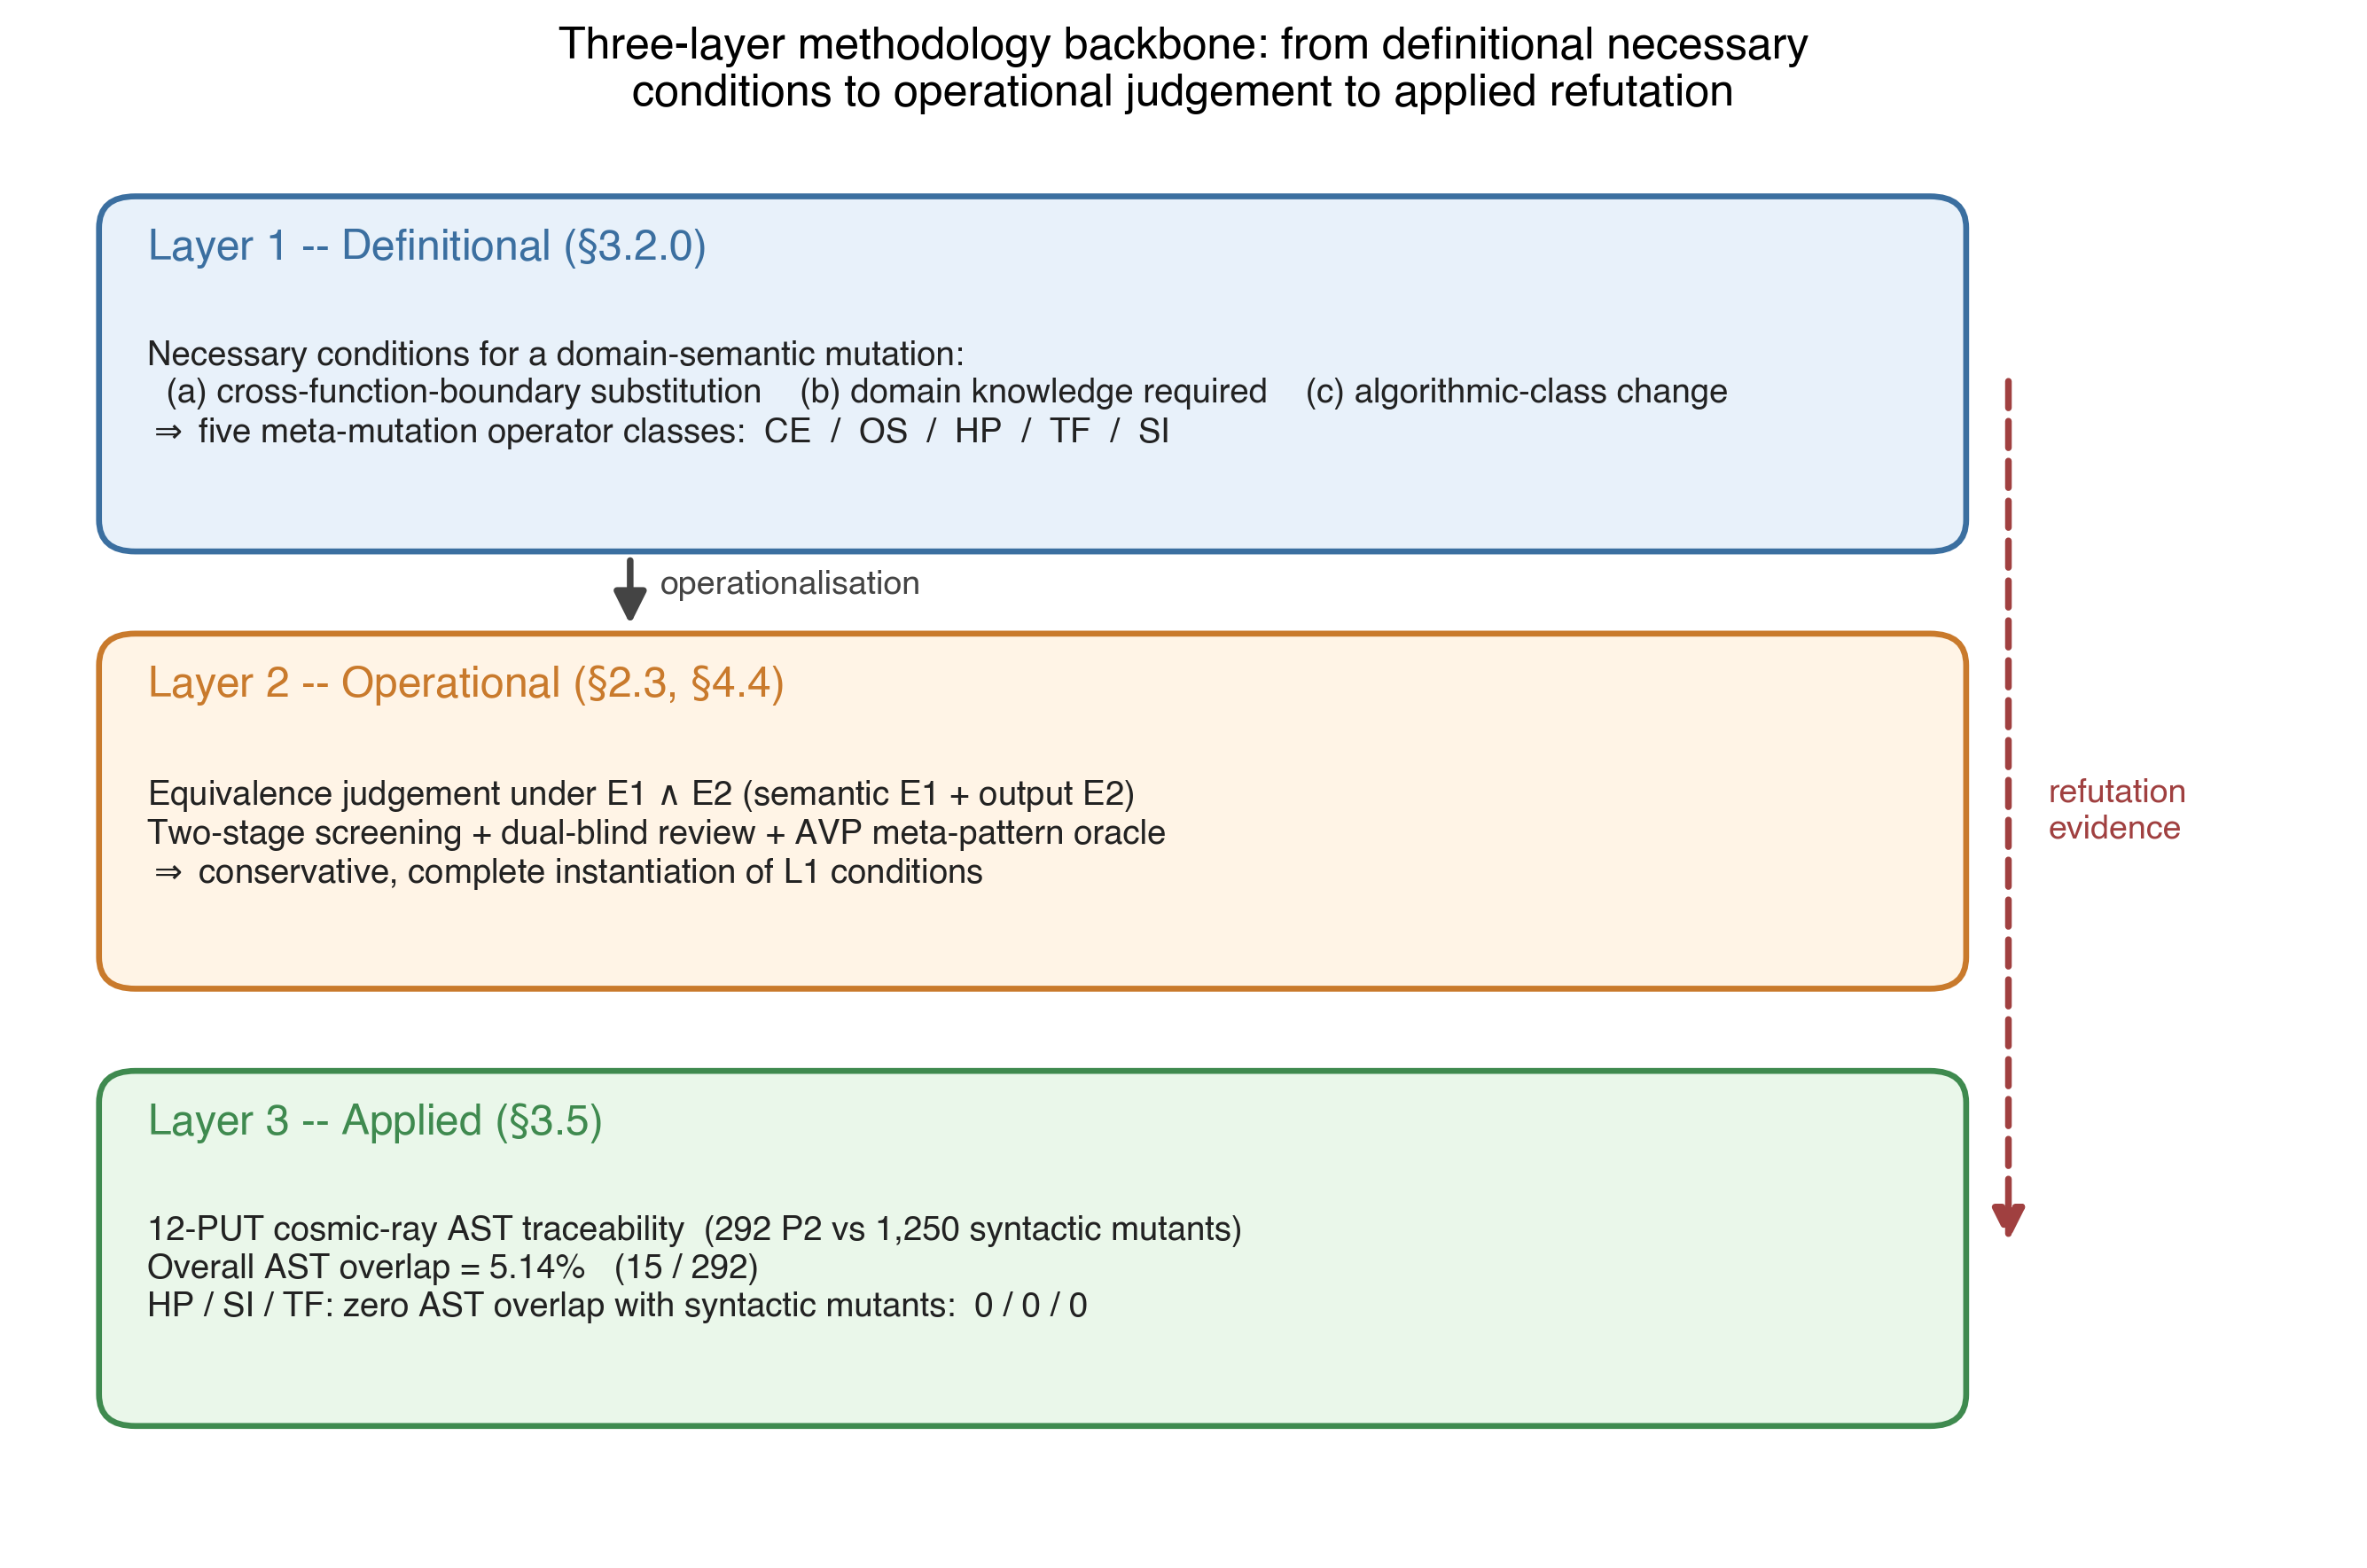
\includegraphics[width=0.48\linewidth,height=0.26\textheight,keepaspectratio,alt={Three-layer methodological framework: Layer 1 (definitional necessary conditions), Layer 2 (operational E\_1 \textbackslash wedge E\_2 judgement), Layer 3 (applied AST-normalised traceability across 12 PUTs).}]{figures/png/fig1_three_layer_methodology.png}
\caption{Three-layer methodological framework: Layer 1 (definitional
necessary conditions), Layer 2 (operational \(E_1 \wedge E_2\)
judgement), Layer 3 (applied AST-normalised traceability across 12
PUTs).}\label{fig:framework}
\end{figure}

\section{Related Work}\label{related-work-and-roadmap}

Seven lines of prior work bracket the contribution of this paper.

General MT foundations and surveys define the oracle-problem setting and
the role of metamorphic relations in paired-test reasoning
\citep{chen2018metamorphic,segura2016survey,liu2014alleviate}. Because
our empirical subject class is scientific computing, we also take the
scientific-software testing survey by \citet{kanewala2014scientific} as
the nearest domain background.

\textbf{(a) Classical mutation testing.} \citet{jia2011analysis} and
\citet{papadakis2019advances} survey syntactic mutation, and the Coupling Effect
Hypothesis (CPH) underpins MS as a fault proxy \citep{demillo1978hints,andrews2005mutation,just2014mutants}.
We argue in Section~\ref{p2-vs-syntactic-mutants-12-put-empirical-layer-3} that
CPH holds within syntactic mutation but does not automatically extend across the
syntactic-versus-domain-semantic boundary, with the 5.14\% AST overlap (HP, SI,
TF at 0/0/0) as the empirical witness. The correctness-versus-test-evidence
concern predates modern mutation score \citep{budd1982correctness}; SMS inherits
it but changes the adequacy object from a test set to an MR set over admitted
semantic mutants.

\textbf{(b) Higher-order mutation.} \citet{jia2009hom} and \citet{kintis2018effective}
study compositions of first-order syntactic mutants. We
explicitly exclude any equivalence claim about Higher-Order Mutation
(HOM) and list HOM equivalence as a residual threat (Appendix F.2).

\textbf{(c) LLM-generated mutants.} Pre-trained-language-model mutation begins
with $\mu$BERT \citep{degiovanni2022mubert}; \citet{tip2025llmorpheus} introduce
LLMorpheus (single-LLM JavaScript mutants), \citet{humbatova2021deepcrime}
DeepCrime (deep-learning real-fault mutation), and \citet{dakhel2024llm} extend
LLM-driven mutation to Java test generation. To our knowledge no prior LLM-mutant
work isolates \emph{LLM source diversity} from \emph{MR design} in the effect
size; the ablation in Section~\ref{cross-source-v4-protocol-summary} closes this
gap. On equivalence, \citet{delgadoperez2020equivalent} emphasise the
\texttt{equiv} term, which we extend to a semantic-class equivalence
E1 $\wedge$ E2 (Section~\ref{equivalence-judgement-e1-e2-layer-2});
\citet{zhang2021classintegration} validate MT in class-integration ordering; and
Meta's ACH \citep{foster2025ach} deploys mutation-guided LLM test generation on
general software, whereas we measure MR adequacy on scientific kernels.

\textbf{(d) Semantic mutation operators across testing communities.}
Semantic mutation predates the LLM-mutant lineage: \citet{clark2010semanticmut}
introduce \emph{semantic mutation testing} distinct from syntactic mutation,
\citet{dan2012smtc} tool it for C, and \citet{derezinska2019uml} apply
\emph{semantic mutation operators} to UML state machines by perturbing
semantic-variation-point interpretations. Their object is the language
interpretation a developer may misread; ours is a certified violation of a
declared domain invariant in code. Within MT, \citet{sun2016mumt,sun2024datamutation}
propose \emph{data mutation operators} and the $\mu$MT methodology,
\citet{zhu2020datamorphic} formalise \emph{datamorphic testing} (separating
datamorphisms from metamorphisms), \citet{chan2024metamorphic} extend generic
data mutation to defect-prediction validation, and \citet{curto2025semanticinvariance}
formalise \emph{semantic invariance} in LLM MT. These establish that mutation can
target data, relation, task, and behavioural semantics.
\textbf{The contribution of this paper is the
first to formalise a domain-specific Semantic Mutation Score (SMS) for
MR adequacy in scientific computing kernels, with a proven
backward-compatible reduction to classical MS (Theorem~\ref{thm:degeneration}) and a
code-level operator framework (Conservation Erosion, Operator
Substitution, Hyperparameter, Trajectory Flip, Structural Injection)
targeting kernel-specific faults, and to delineate the strong boundary
of metamorphic-relation grounding, a strong/weak MR distinction whose
$\varepsilon_{\mathrm{tol}}$-governed duality (Theorem~\ref{thm:duality}, Proposition~\ref{prop:boundary})
is mapped empirically on real and textbook programs spanning the
meta-patterns (Section~\ref{rq4-strong-boundary}), complemented by a cross-library adjoint extension
arm (Section~\ref{adjoint-extension-arm-subjects}, Section~\ref{rq4-adjoint-extension-arm}) that supports the duality forward on third-party
linear operators with real fixed defects.}

\textbf{(e) MR adequacy and coverage.} Recent MT adequacy work, separated by its
\emph{counting object}: \citet{xiang2019compositeMR} build composite MRs but
evaluate with the classical MuJava syntactic-mutant denominator;
\citet{fu2024mtadequacy} define MT adequacy over MR obligations and source
inputs; \citet{liu2024mtcoverage} integrate MR coverage; and
\citet{ba2025metamorphiccoverage} define Metamorphic Coverage over
differentially executed code elements, all denominators being obligations,
source-tests, or execution coverage rather than semantic mutant classes.
\citet{xie2024mutmodel} quantify MR diversity (MUT), and
\citet{huang2022mrprioritization,zhang2022effectivemrselection} rank/select MRs
by validity, coverage, or mutation-score, all boundary surrogates rather than an
adequacy fraction over enumerated semantic fault classes.
\citet{alblwi2023semanticcoverage} give a non-MT semantic-coverage analogue on
the test-suite side. None makes the denominator the admitted nonequivalent
\emph{domain-semantic code mutants} for scientific kernels or establishes
compatibility with the classical MS denominator; SMS differs by replacing the
denominator against which an MR set is judged, not by proposing another coverage
metric.

\begin{table}[t]
\centering
\footnotesize
\caption{Closest denominator-oriented comparators to SMS. The comparison
is by adequacy object and denominator semantics, not by whether a paper
uses the phrase metamorphic-testing adequacy.}
\label{tab:closest-denominator-comparators}
\begin{tabularx}{\textwidth}{p{0.22\textwidth}p{0.34\textwidth}X}
\toprule
Work & Denominator or counted object & Relation to SMS \\
\midrule
\citep{fu2024mtadequacy,liu2024mtcoverage} & MR obligations, MR coverage, and source-test obligations & Closest MR/MT adequacy comparators, but property/coverage denominators rather than semantic mutant classes \\
\citep{ba2025metamorphiccoverage} & Differentially executed code elements in paired MT runs & Execution-side coverage comparator, not MR-set semantic adequacy \\
\citep{xie2024mutmodel} & MR feature/diversity space & Boundary surrogate for MR-set quality, not an adequacy fraction over faults or semantic classes \\
\citep{huang2022mrprioritization,zhang2022effectivemrselection} & MR validity, coverage, and classical mutation-score signals & Boundary surrogate for cost-effective MR choice, not a denominator-bearing adequacy metric \\
\citep{alblwi2023semanticcoverage} & Semantic obligations under a specification & Non-MT semantic-coverage analogue; test-suite side rather than MR-set side \\
\bottomrule
\end{tabularx}
\end{table}

\textbf{(f) Property-relative and numerical-specification mutation.}
Recent property-aware mutation work moves the adequacy question closer
to requirements and invariants: \citet{bartocci2023propertymut} make mutant
relevance and meaningful killing relative to a tested property, and
\citet{jeangoudoux2021interval} generate tests for numerical
specifications through interval-constraint reasoning over floating-point
accuracy and robustness requirements. These works are closer to SMS than
generic AST mutation because they reject property-irrelevant mutants as
an adequacy denominator. They still differ from the present paper in
three respects: the adequacy object here is an MR set rather than a
single formal requirement, the denominator is a five-class
domain-semantic mutant space for scientific kernels, and the metric is
constructed as a backward-compatible generalisation of MS.

\textbf{(g) Semantic foundations and the certificate gap.} Abstract
interpretation supplies the standard machinery for relating concrete
semantics to abstract domains and invariant families \citep{cousot1992absint},
and for designing program transformations by their effect on an
abstract semantics \citep{cousot2002transform}. Approximate program
transformation semantics gives a second, quantitative route: local error
expressions and partial-metric semantics can certify that a
transformation lies within a bounded semantic-effect envelope \citep{westbrook2013approx,geoffroy2021partialmetric}. Refinement- and
UTP-based mutation testing lift mutation to contracts and
specifications \citep{aichernig2002contract,aichernig2007utp}, while
usage-aware differential dynamic logic tracks admissible proof-level
mutations under soundness conditions \citep{dotzel2023usageaware}. These foundations supply much of the machinery needed for
certificate-bearing semantic-effect classes, but they are not MR
adequacy metrics for scientific-computing kernels. Conversely, SMS
provides the MR adequacy denominator and empirical audit, but its
certification layer is empirical and structural rather than
machine-checkable proof-carrying.

\textbf{Closest comparison.} The closest adjacent work is the
Min-MR-Complete formulation \citep{li2026minmrcomplete}, which uses
the same semantic-mutation family as the fault model for MR-subset
completeness and identifies when class-level reasoning collapses to a
mutant-level set-cover problem. The present paper differs in role: it
defines the SMS denominator, the E1 $\wedge$ E2 admission judgement, the
AST-normalised syntactic-unreachability audit, and the empirical
same-source/cross-source ablation. Min-MR-Complete optimises over an
admitted mutant--draw coverage universe; this paper constructs and
audits that universe. Taken together, the two papers come closest to
semantic-effect-class denominators for MR adequacy, but neither yet
attaches a per-mutant machine-checkable certificate showing that a
syntactic edit belongs to a declared abstract semantic-effect class.
Throughout this paper, a certificate is a recorded, budget-stamped
piece of test evidence, not a proof object (Limitation 9); the
undecidability result is precisely why nothing stronger is available.

The SMS metric is conceptually complementary to the code-verification
scope of ASME V\&V 20-2009 §3, which targets numerical-solver
correctness. SMS targets MR fault-detection adequacy; we make no
normative compliance claim (Appendix E.3 records this as a long-term
aspiration only).

\section{Problem Formulation and Semantic Mutation Model}\label{research-questions-and-hypotheses}

This section turns the problem into auditable research questions before the
metric: scope and novelty are stated as RQ1--RQ2, while RQ3--RQ5 test whether one
empirical instantiation is usable, discriminative, and consistent enough to
support the construct.

\subsection{Research Questions}\label{research-questions}

The questions run from the theoretical foundation (RQ1), through the structural
separation (RQ2), to the 60-cell demonstration (RQ3--RQ5). RQ1 is answered by
construction and proof (Sections~\ref{theory-setting}--\ref{theory-fibers}:
Theorem~\ref{thm:undecidability}, Proposition~\ref{prop:fiber},
Theorem~\ref{thm:duality}, and the degeneration of
Section~\ref{sms-ms-degeneration-formal-statement}); RQ2 by the AST audit
(Section~\ref{p2-vs-syntactic-mutants-12-put-empirical-layer-3}); RQ3--RQ5 by the
pre-registered pipeline (Section~\ref{statistical-analysis-and-empirical-results}),
mirroring the three-layer framework (Layer 1 carries RQ1, Layer 3 RQ2).

\begin{itemize}
\tightlist
\item
  \textbf{RQ1 (Theory of semantic mutation: constructibility,
  undecidability, duality, backward compatibility).} Can semantic
  mutation be formalised as a fiber decomposition of a single effect map
  over admitted nonequivalent \emph{domain-semantic code mutants} for
  scientific-computing kernels, such that (a) stratum membership is
  undecidable and therefore certificate-based (Theorem~\ref{thm:undecidability}), (b) the
  induced adequacy metric SMS degenerates almost everywhere to the
  classical Mutation Score (Proposition~\ref{prop:fiber}; Theorem~\ref{thm:degeneration}), and (c)
  strong metamorphic relations detect only the semantically active
  mutants within a tolerance-bounded regime, while outside it the duality
  degrades along an $\varepsilon_{\mathrm{tol}}$-governed strong boundary
  into false positives (weak MRs, where a correct discrete program
  violates the invariant) and false negatives (surviving non-equivalent
  mutants under coincidental satisfaction) (Theorem~\ref{thm:duality} and Proposition~\ref{prop:boundary};
  the boundary is mapped empirically under RQ4)?
\item
  \textbf{RQ2 (Syntactic unreachability).} To what extent is the
  domain-semantic mutant space induced by the five operators reachable
  by default-configuration first-order syntactic mutation tools at the
  AST-normalised level?
\item
  \textbf{RQ3 (Instantiability).} Do the five semantic mutation
  operators instantiate a usable nonequivalent semantic-mutant
  denominator across the 60 PUT-MP-operator cells, as reflected by
  inst\_rate, equiv\_rate, C1\_share, and survive\_rate?
\item
  \textbf{RQ4 (Discrimination, LLM-source decoupling, the strong boundary, and
  industrial construct separation).} Does SMS discriminate aligned (j=k) from
  cross (j$\neq$k) slices; does cross-source pooling under an identical prompt
  move the effect size or only the kill-set quality; where does the strong
  boundary of Proposition~\ref{prop:boundary} lie empirically (where does a
  strong MR kill the genuine fault and where does the duality fail as a weak-MR
  false positive or a surviving non-equivalent mutant); and does the construct
  separation among kill-rate, semantic alignment, and real-defect detection
  remain visible on an industrial arm of reproduced, MR-detectable library
  defects?
\item
  \textbf{RQ5 (Cross-class consistency).} Does the aligned-versus-cross
  SMS pattern generalise across four representative classes of
  single-output scientific-computing kernels? (The relationship between
  SMS and the coverage-style surrogate Pattern Coverage is reported
  descriptively at n = 12 as a hypothesis-generating observation, not a
  confirmatory test.)
\end{itemize}

\subsection{Hypotheses}\label{hypotheses}

The empirical questions RQ3--RQ5 carry pre-registered hypotheses; RQ1 is
answered by Theorem~\ref{thm:degeneration} and RQ2 by the Section~\ref{p2-vs-syntactic-mutants-12-put-empirical-layer-3} structural audit, neither of
which is a statistical hypothesis.
The hypothesis definitions, primary-MR convention, and statistical
reporting hierarchy are frozen in
\texttt{docs/experiment\_documentation/EXPERIMENT\_DESIGN.md} at commit
\texttt{0f2509527f346f9433c3cf90959bb07d80601a23} and in the Zenodo
replication package
\href{https://doi.org/10.5281/zenodo.20250664}{10.5281/zenodo.20250664}.

\begin{itemize}
\tightlist
\item
  \textbf{H1 (RQ3).} At least 4 of the 5 operators produce $\geq$ 5 non-equivalent
  mutants on at least 9 of the 12 PUTs.
\item
  \textbf{H2 (RQ4; pre-registered as an exploratory large-effect
  target).} The aligned-SMS to
  cross-SMS odds ratio is $\geq$ 3.0, and Cliff's $\delta$ is $\geq$ 0.474.
  The threshold was fixed before data collection, but the design is
  underpowered at this boundary, so its verdict is read as a
  point-estimate result
  (stipulated-alternative power in Section~\ref{rq2-stipulated-alternative-power}), not
  a confirmatory claim of the paper.
\item
  \textbf{H3 (RQ5).} A within-class sign test gives 4/4 across the 4 classes,
  and CV($\Delta$SMS) \textless{} 0.5.
\item
  \textbf{H4 (RQ4).} Mean suspect\_share is $\leq$ 0.20 across the 60 cells.
\end{itemize}

\textbf{What would count against the construct (stated post hoc).} The
pre-registered thresholds stress one instantiation and do not exhaust
falsifiability. The construct itself would be disconfirmed by: (i) the
degeneration path failing empirically, with SMS and MS disagreeing on
the same pools in the syntactic limit; (ii) the aligned-versus-cross
direction reversing systematically across designs; (iii) the industrial
arm showing the generic baselines' kill sets nesting the pattern-derived
kill sets, leaving no construct separation; or (iv) certificates failing
audit, with declared strata not matching observed effects. Criteria
(ii)--(iv) were observed not to occur; criterion (i) was not directly
tested and is open to replication. We state these criteria post hoc,
after the verdicts, and label them accordingly.

The 12 PUTs are deliberately \emph{Numerical Recipes}--style compact
kernels: they provide a verifiable minimum working example for the
three-layer backbone, while industrial-scale transfer is left to future
work under the representativeness threat.

% [thematic break removed]

\subsection{Formal Model and Semantic Mutation Score}\label{notation-and-equivalence-judgement}

\subsubsection{Vocabulary and Notation}\label{vocabulary-inheritance}

We use a small vocabulary throughout the method. The terms are declared
here before they are used in the SMS construction.

\textbf{Program Under Test (PUT).} A PUT is the scientific-computing
kernel being assessed. We write the \(i\)-th PUT as \(S_i\).

\textbf{Metamorphic Relation (MR).} An MR is a property that relates the
outputs of related inputs. The MR battery used for PUT \(S_i\) and
meta-pattern \(k\) is written \(\mathrm{MR}_{i,k}\): the concrete set of
executable MR instances exercised on one subject at one stratum. The
registered infrastructure documents historically call this object an
``MR family''; we say \emph{battery} in prose because the companion
framework NOETHER \citep{noether2026} reserves \emph{MR family} for a
coarser object, a program-family-level class of executable MRs
instantiating one MetaPattern. In NOETHER's symbols a MetaPattern is
\(m_{\bullet}\), an MR family is \(\mathsf{f}_{\bullet}\), and an
executable MR is \(\rho_{\bullet}\); our \(\mathrm{MR}_{i,k}\) is a
per-PUT set of such \(\rho\)-level instances, one granularity below
NOETHER's family layer.

\textbf{Meta-pattern (MP).} An MP is a semantic stratum of MR behaviour,
such as conservation, monotonicity, convergence, trajectory structure, or
fidelity order. The index \(k\) denotes the MP being tested.

The five meta-patterns are instances, on the scientific-computing program
family, of five MR families in the two-layer taxonomy of NOETHER
\citep{noether2026}. From a program-induced operator algebra NOETHER derives
five Layer-1 MetaPatterns, \(m_{\mathrm{inv}}\), \(m_{\mathrm{mono}}\),
\(m_{\mathrm{adj}}\), \(m_{\mathrm{rev}}\), and \(m_{\mathrm{conv}}\), and ten
Layer-2 MR families instantiating them; two structural refinements
(\(\mathcal{D}^{*}\), \(\mathcal{E}^{*}\)) and one relational extension enter
at the family layer rather than adding MetaPatterns. Our grid is stratified at
the family layer. We record the correspondence to our registered labels once,
here: MP1 conservation \(= \mathsf{f}_{\mathrm{inv.con}}\) (under
\(m_{\mathrm{inv}}\), group action \(G\)); MP2 monotonicity
\(= \mathsf{f}_{\mathrm{mono.stat}}\) (under \(m_{\mathrm{mono}}\), partial
order \(O_{\le}\)); MP3 convergence order \(= \mathsf{f}_{\mathrm{conv.lim}}\)
(under \(m_{\mathrm{conv}}\), limit operator \(\mathcal{L}^{*}\)); MP4
trajectory determinism \(= \mathsf{f}_{\mathrm{mono.shape}}\) (the
\(\mathcal{D}^{*}\) qualitative-dynamics refinement, under
\(m_{\mathrm{mono}}\)); and MP5 partial-order consistency
\(= \mathsf{f}_{\mathrm{conv.rate}}\) (the \(\mathcal{E}^{*}\)
method-comparison refinement, under \(m_{\mathrm{conv}}\); Mode-M,
implementation-orbit, in NOETHER's classification). The adjoint extension
\(\psi_6\) instantiates \(\mathsf{f}_{\mathrm{adj.self}}\) (under
\(m_{\mathrm{adj}}\), self-adjoint operator \(T^{*}\)). The six strata thus
cover six of NOETHER's ten MR families and four of its five MetaPatterns
(time reversal, \(m_{\mathrm{rev}}\), is not exercised). The registered labels
MP1--MP5 are retained throughout for every pre-registration, dataset-key, and
provenance reference, because the pre-registered protocol was authored under
those labels and only under those labels; NOETHER's family names carry the
semantic narrative and never stand in for a registration.

\textbf{Semantic operator.} A semantic operator is a mutation family
\(\mathrm{mut}_j\) designed to perturb a declared MP. The operator index
\(j\) identifies the intended semantic effect.

\textbf{Semantic mutant.} A semantic mutant \(s'\) is a finite syntactic
edit of \(S_i\) that is admitted by semantic operator \(\mathrm{mut}_j\)
and is certified against the declared MR battery. Formally,
\[
  s' \in \mathrm{mut}_j(S_i).
\]
The word semantic therefore names the certification target, not a second
editing mechanism.

\textbf{Semantic-effect fiber.} For an MR battery \(\mathrm{MR}_{i,k}\),
the semantic-effect fiber is the subset of admitted semantic mutants
whose declared effect is observable by that MR battery:
\[
  \mathcal{F}(\mathrm{MR}_{i,k}) =
  \{s' \in \mathrm{mut}_j(S_i): \mathrm{killed}(s', \mathrm{MR}_{i,k})\}.
\]
Different MR batteries can observe different fibers. SMS therefore
measures adequacy relative to a declared stratum; it is not a total order
over all possible MR batteries.

\textbf{Equivalent, killed, and surviving mutants.} A mutant is
equivalent for \((i,k,j)\) when the equivalence judgement of Section~\ref{equivalence-judgement-e1-e2-layer-2} admits
it into \(\mathrm{equiv}_{i,k,j}\). A non-equivalent mutant is killed when
at least one MR in \(\mathrm{MR}_{i,k}\) passes on \(S_i\) and fails on
\(s'\). A non-equivalent mutant that is not killed is surviving. Thus
the generated mutant set decomposes as:

\begin{align*}
\mathrm{mut}_j(S_i) &= \mathrm{equiv}_{i,k,j} \cup \mathrm{killed}_{i,k,j} \cup \mathrm{survive}_{i,k,j} \quad \text{(disjoint)} \\
\mathrm{SMS}_{i,k,j} &:= \frac{|\mathrm{killed}_{i,k,j}|}{|\mathrm{mut}_j(S_i)| - |\mathrm{equiv}_{i,k,j}|} \in [0,\,1]
\end{align*}

\textbf{Semantic Mutation Score (SMS).} SMS preserves the classical
Mutation Score (MS) ratio while replacing the internal definitions of
mutant generation, equivalence, and killing with MR-relative semantic
definitions. The classical concepts of mutation operator, mutant,
equivalent mutant, killed mutant, surviving mutant, and MS are inherited
from \citet{jia2011analysis} and
\citet{ammann2008introduction}.

The complete notation table is in Appendix A.1; index sets and tolerance
parameters ($\varepsilon_{\mathrm{eq}}$, $\varepsilon_{\mathrm{AVP}}^k$,
$K_{\mathrm{eq}} = 1000$, $N = 20$) follow that table.

\subsubsection{Semantic-Operator Signatures}\label{operator-signatures}

Operator family and alignment:

\begin{align*}
\mathrm{MUT} &= \{\mathrm{mut}_C,\, \mathrm{mut}_M,\, \mathrm{mut}_G,\, \mathrm{mut}_T,\, \mathrm{mut}_F\} \quad \text{(open, extensible)} \\
\mathrm{mut}_j &: \text{Programs} \to 2^{\text{Programs}} \\
\mathrm{align}(j) &= j \quad \text{(design choice, not theorem)}
\end{align*}

\begin{table}[t]
\caption{Operator signatures.}\label{tab:p2-01}
\centering
\begin{tabular}{@{}lll@{}}
\toprule
Operator & Failure semantics & Aligned MP \\
\midrule
mut\_C & Conservation-breaking & MP\_1 Conservation \\
mut\_M & Monotonicity-breaking & MP\_2 Monotonicity \\
mut\_G & Convergence-breaking & MP\_3 Convergence \\
mut\_T & Trajectory-distorting & MP\_4 Trajectory \\
mut\_F & Fidelity-order-breaking & MP\_5 Partial-order \\
\bottomrule
\end{tabular}
\end{table}

Per-PUT specialisation tables (mut\_C/M/G/T/F across 12 PUTs and 4
classes) are deferred to \textbf{Appendix B.2}.

\subsubsection{Equivalence Judgement}\label{equivalence-judgement-e1-e2-layer-2}

The equivalence judgement is the executable instantiation of the Layer-1
necessary conditions (Section~\ref{necessary-conditions-for-semantic-mutation-layer-1}). For each candidate mutant
\texttt{s\textquotesingle{}}:

\begin{itemize}
\tightlist
\item
  \textbf{E1 (AVP-coherent):} $\forall$ mr $\in \mathrm{MR}_{i,k}$: $\mathrm{AVP}(S_i, mr)$ =
  $\mathrm{AVP}(s', mr)$.
\item
  \textbf{E2 (Output-equivalent):} $\forall$ x in $K_{\mathrm{eq}}=1000$ samples
  $\sim D_S$: $\|S_i(x) - s'(x)\| \leq \varepsilon_{\mathrm{eq}}$.
\end{itemize}

E1 $\wedge$ E2 is the conservative complete instantiation: false-equiv (a
truly non-equivalent mutant admitted as equivalent) requires \emph{both}
AVP coherence and numerical agreement on K\_eq samples to hold despite the
non-equivalence (both mis-pass simultaneously), which is rare;
false-non-equiv requires only one of E1, E2 to fail for a truly equivalent
mutant, biasing SMS slightly low: a misjudged equivalent mutant remains in
the denominator as an unkillable survivor, understating adequacy. The
trade-off table against
E1-alone and E2-alone is in Appendix A.3. Under the $L_{\mathrm{equiv}}$
component (L1 $\wedge$ L2) of the Section~\ref{sms-ms-degeneration-formal-statement} degenerate
limit, E1 $\wedge$ E2 reduces almost everywhere to classical bitwise
equivalence (Lemma G.1, supplementary Appendix G).

\paragraph{Semantic certificate record.}
For each admitted mutant, the empirical certificate is a structured
record rather than a proof-carrying object. The record contains the PUT
identifier, operator identifier, intended meta-pattern stratum, edit
class, targeted semantic invariant, E1 AVP-coherence result, E2 sampling
budget and tolerance, killed/survived vector over the relevant MRs, LRCA
labels for killed outcomes, generation source and reviewer status, and a
trace path to the reproduced artifact. A mutant enters the SMS
denominator only after the record passes the Layer-1 semantic-condition
check and the E1 $\wedge$ E2 equivalence judgement. LRCA labels remain
diagnostic annotations on the certificate; they do not filter the
denominator or redefine SMS.

The killed determination preserves the classical OR-aggregation:

\[
\begin{aligned}
\mathrm{killed}(s', \mathrm{MR}_{i,k}) \iff{} & \exists\,mr \in \mathrm{MR}_{i,k}: \\
& \mathrm{AVP}(S_i, mr) = \text{pass} \wedge
  \mathrm{AVP}(s', mr) = \text{fail}.
\end{aligned}
\]

\subsubsection{Root-Cause Diagnostic Layer}\label{lrca-engineering-attribution-layer-descriptive-not-in-sms}

Likely Root-Cause Analysis (LRCA) annotates every killed mutant with one
of five diagnostic labels: C1 likely semantic failure, C2
numerical-tolerance perturbation, C3 out-of-distribution (OOD) trip, C4
statistical-assumption violation, and C5 mutator artefact. The diagnostic
procedure is a three-layer decision tree.
Layer 1 checks tolerance robustness over N = 20 repeats with a
fail-ratio cutoff of 0.80. Layer 2 triages OOD on the surrogate and
machine-learning classes. Layer 3 checks statistical-assumption
baselines on the probabilistic and machine-learning classes using
Wilcoxon and Dynamic Time Warping. A final pass rechecks for mutator
artefacts. Multiple labels are resolved by priority C5 \textgreater{} C4
\textgreater{} C3 \textgreater{} C2 \textgreater{} C1.

The output quantities are \texttt{C1\_share} (share of C1 among killed
mutants) and \texttt{suspect\_share\ :=\ 1\ −\ C1\_share}. \textbf{LRCA
does not modify the SMS formula}: the killed set is never filtered by
suspect status. LRCA is a diagnostic annotation that indicates
whether a given kill is more consistent with a semantic-failure
detection, tolerance sensitivity, OOD behaviour, statistical-assumption
failure, or mutator artefact. Appendix A.2 gives the full decision tree, the 9-grid
threshold calibration, and the engineering rationale for the priority
ordering.

\subsubsection{Backward-compatibility declaration}\label{backward-compatibility-declaration}

The seven core concepts (PUT, mutation operator, mutant, equivalent
mutant, killed mutant, surviving mutant, mutation score) and the SMS
formula
\texttt{\textbar{}killed\textbar{}\ /\ (\textbar{}mut\textbar{}\ −\ \textbar{}equiv\textbar{})}
are aligned item-for-item with \citet{jia2011analysis}. We extend only the
internal definitions: \texttt{mut} shifts from syntactic to
domain-semantic operators, \texttt{equiv} shifts from bitwise
behavioural equivalence to the semantic-class equivalence E1 $\wedge$ E2, and
\texttt{killed} shifts from an equality oracle to a meta-pattern AVP. We
introduce no new formula terms and no new state classifications.

Under the degenerate limit $L$ defined in Section~\ref{sms-ms-degeneration-formal-statement}, SMS reduces
almost everywhere to classical syntactic MS, equivalent mutants
degenerate to classical behavioural equivalence, and killed mutants
degenerate to bitwise difference detection. LRCA labels are diagnostic
annotations outside the SMS formula
(Section~\ref{lrca-engineering-attribution-layer-descriptive-not-in-sms}),
so the metric-level claim does not rest on the diagnostic layer. Any
SMS-based empirical conclusion is therefore structurally consistent with
the existing mutation-testing literature in the classical
syntactic-mutation regime, so there is no metric-level semantic
fragmentation. The skeleton of eleven concepts, the three-state
decomposition, the SMS formula, and the AVP interface are fixed; the
contents of MUT, MP, C, and $\mathrm{cls}$ remain open to future
extension.

\subsubsection{Degeneration to Classical Mutation Score}\label{sms-ms-degeneration-formal-statement}

The Section~\ref{backward-compatibility-declaration} backward-compatibility claim is formalised as a degeneration
theorem. The full notation cross-reference is \textbf{Appendix G.1}; the joint
conditions are in \textbf{Appendix G.2}, the lemma proofs in
\textbf{Appendix G.3}, and the full theorem proof in \textbf{Appendix G.4}. We
state only the main theorem here; the three construction
lemmas are stated and proved in the supplementary material as
Lemma G.1--G.3, each under exactly its own joint condition.

\textbf{Definition (Degenerate limit).}
$L = L_{\mathrm{equiv}} \wedge L_{\mathrm{killed}} \wedge L_{\mathrm{mut}}$, where each joint
condition is a pair of paired axes acting on one layer of the SMS
formula:

\begin{itemize}
\tightlist
\item
  $L_{\mathrm{equiv}} = L1 \wedge L2$: $\varepsilon_{\mathrm{eq}} \to 0 \wedge K_{\mathrm{eq}} \to \infty$ (controls equiv
  layer; Lemma G.1).
\item
  $L_{\mathrm{killed}} = L3 \wedge L4$: $\varepsilon_{\mathrm{AVP}} \to 0 \wedge$ MP set = $\{\mathrm{MP}_{\mathrm{eq}}\}$
  (controls killed layer; Lemma G.2).
\item
  $L_{\mathrm{mut}} = L5 \wedge L6$: $\mathrm{mut}_j$ switches to rule-based syntactic
  operators (Mothra-style, or modern MutMut/PIT-style) $\wedge$ PUT class $\subseteq$ imperative deterministic
  programs (controls mut layer; Lemma G.3).
\end{itemize}

\begin{theorem}[SMS $\to$ MS degeneration]\label{thm:degeneration}
In the degenerate limit
$L$, \textbf{almost everywhere} with respect to the input
distribution $D_S$,

\[ \mathrm{SMS}_{i,k,j} \xrightarrow{L} \mathrm{MS}_{i,j} = \frac{|\mathrm{killed}_{i,j}^{\mathrm{classic}}|}{|\mathrm{mut}_j^{\mathrm{syntax}}(S_i)| - |\mathrm{equiv}_{i,j}^{\mathrm{classic}}|} \]

where the right-hand side is the classical Mutation Score of
\citet{jia2011analysis},
$\mathrm{killed}^{\mathrm{classic}}$ is the difference-detection set,
$\mathrm{equiv}^{\mathrm{classic}}$ is the behavioural-equivalence set,
and $\mathrm{mut}^{\mathrm{syntax}}$ is the syntactic-mutant set.
\end{theorem}

\begin{proof}[Proof sketch]
By Lemma G.1, under $L_{\mathrm{equiv}}$ (L1 $\wedge$ L2) alone the E2 arm
of the E1 $\wedge$ E2 judgement (Section~\ref{equivalence-judgement-e1-e2-layer-2})
forces pointwise output equality almost everywhere with respect to
$D_S$, and the E1 arm (AVP coherence) is then implied outside the same
measure-zero set, so
$\mathrm{equiv}_{i,k,j} \to \mathrm{equiv}_{i,j}^{\mathrm{classic}}$
almost everywhere; the measure-zero qualifier accommodates
floating-point pathological points and Not-a-Number propagation. By
Lemma G.2, under $L_{\mathrm{killed}}$ (L3 $\wedge$ L4) alone,
$\mathrm{killed}_{i,k,j} \to \mathrm{killed}_{i,j}^{\mathrm{classic}}$,
and the MP index $k$ degenerates because L4 collapses
$\mathrm{MR}_{i,k}$ to $\{\mathrm{MP}_{\mathrm{eq}}\}$. By Lemma G.3,
under $L_{\mathrm{mut}}$ (L5 $\wedge$ L6) alone,
$\mathrm{mut}_j(S_i) \to \mathrm{mut}_j^{\mathrm{syntax}}(S_i)$. Each
lemma uses only its own joint condition, so no step of the composition
invokes an assumption outside its stated level. Substituting the three
limits into the SMS formula gives $\mathrm{MS}_{i,j}$. Full lemma
proofs are in supplementary Appendix G.3 and the full theorem proof in
supplementary Appendix G.4.
\end{proof}

Under the stated substitutions the equality is definitional once the
three layers coincide; the almost-everywhere qualifier concerns only
the bounded E2 classifier on floating-point pathological inputs. We
therefore read Theorem~\ref{thm:degeneration} as a
backward-compatibility characterisation of SMS, not as an independent
mathematical contribution.

The diagnostic LRCA layer sits outside the SMS formula
(Section~\ref{lrca-engineering-attribution-layer-descriptive-not-in-sms}),
so Theorem~\ref{thm:degeneration} carries the backward-compatibility
claim on its own; whether the root-cause inventory also collapses to
\{C1\} under $L$ depends on the engineering thresholds of the LRCA
decision tree and is not claimed formally.

\textbf{Empirical consistency.} Theorem~\ref{thm:degeneration}
shows that the SMS-based empirical conclusions (Section~\ref{statistical-analysis-and-empirical-results} Cliff's delta,
Friedman chi\^{}2, Spearman rho) are structurally consistent with
existing mutation-testing literature in the classical syntactic-mutation
regime, and \textbf{do not} constitute metric-level semantic
fragmentation.

% [thematic break removed]

\subsubsection{Semantic-Mutation Theory Setting}\label{theory-setting}

The preceding subsections fix the SMS metric and its degeneration to MS; we now
give the theory it instantiates. Semantic mutation is \emph{intensionally
semantic, extensionally syntactic}: every mutation is mechanically a syntactic
act (semantics changes only through syntax), and what makes a mutant
\emph{semantic} is where its defining condition lives (a specified invariant
violation at the semantic layer) and how its membership is established (by
certificate, because the condition is undecidable).

Fix a grammar $G$ and the set $\mathrm{Prog}(G)$ of well-formed programs
with denotational semantics
$\llbracket\cdot\rrbracket : \mathrm{Prog}(G) \to (\mathcal{X} \rightharpoonup \mathcal{Y})$.
Let $\alpha : \mathcal{Y} \to \mathcal{Y}_\alpha$ be the committed
semantic abstraction (the observable that the AVP of Section~\ref{equivalence-judgement-e1-e2-layer-2} reads), and
write $P \equiv_\alpha P'$ when
$\alpha \circ \llbracket P \rrbracket = \alpha \circ \llbracket P' \rrbracket$
pointwise on the admitted input domain $\mathcal{X}_{\mathrm{adm}}$.
This $\equiv_\alpha$ is exactly the equivalent-mutant relation
$\mathrm{equiv}$ of Section~\ref{vocabulary-inheritance}: the E2 component of the E1$\wedge$E2 judgement
(Section~\ref{equivalence-judgement-e1-e2-layer-2}) is its bounded decision procedure on $K_{\mathrm{eq}}$ samples.

The new ingredient is a finite \emph{semantic invariant family}
$I = \{\psi_1, \dots, \psi_5\}$, where each $\psi$ is a predicate over
the observable behaviour $\alpha \circ \llbracket P \rrbracket$. The five
invariants are exactly the properties the meta-patterns of Section~\ref{operator-signatures} target:
$\psi_1$ conservation ($\mathsf{f}_{\mathrm{inv.con}}$), $\psi_2$ monotonicity
($\mathsf{f}_{\mathrm{mono.stat}}$), $\psi_3$ convergence order
($\mathsf{f}_{\mathrm{conv.lim}}$), $\psi_4$ trajectory determinism
($\mathsf{f}_{\mathrm{mono.shape}}$), $\psi_5$ partial-order
consistency ($\mathsf{f}_{\mathrm{conv.rate}}$), so
$\psi_k$ is the invariant whose violation MP$_k$ detects and whose
breakage $\mathrm{mut}_j$ (at $j=k$) targets; each $\psi_k$ is thus the
defining invariant of the NOETHER MR family named in parentheses
\citep{noether2026}. We write
$\llbracket P \rrbracket \models \psi$ when $P$'s observable behaviour
satisfies $\psi$.

The family is open (the extensibility of $I$ noted in Section~\ref{theory-fibers}): a sixth
invariant $\psi_6$, \emph{adjoint consistency} ($\mathsf{f}_{\mathrm{adj.self}}$,
the self-adjoint family under MetaPattern $m_{\mathrm{adj}}$, operator $T^{*}$,
in NOETHER \citep{noether2026}),
$\langle A x, y\rangle = \langle x, A^{\mathrm{H}} y\rangle$ for
linear-operator kernels, instantiates the same construction. Its MR is
strong (its violation set is closed under $\equiv_\alpha$), so by
Theorem~\ref{thm:duality} it detects only the semantically active mutants of the adjoint code
path. Because adjoint consistency is meaningful only for linear operators
, not for the chaotic, stochastic, and nonlinear machine-learning
kernels that make up most of the 12 PUTs, $\psi_6$ is \emph{not} folded
into the pre-registered 60-cell design (doing so would leave the invariant
undefined on ten of the twelve subjects); it is instead demonstrated as a
separate confirmatory \emph{adjoint extension arm} on dedicated
third-party linear-operator subjects (Section~\ref{adjoint-extension-arm-subjects}, Section~\ref{rq4-adjoint-extension-arm}), leaving the
pre-registered hypotheses H1--H4 untouched.

\subsubsection{Semantic-Mutant Conditions}\label{theory-s1s5}

The following certified definition is the formal counterpart of the
informal Layer-1 necessary conditions of Section~\ref{necessary-conditions-for-semantic-mutation-layer-1}.

\textbf{Definition (semantic mutant).} Given $(P, \psi)$ with
$\llbracket P \rrbracket \models \psi$, a program $P'$ is a
\emph{semantic mutant of $P$ at stratum $\psi$} iff: (S1)
\emph{realizability}, $P' = e(P)$ for a finite AST edit $e$; (S2)
\emph{baseline}, $\llbracket P \rrbracket \models \psi$; (S3)
\emph{violation with witness},
$\llbracket P' \rrbracket \not\models \psi$, witnessed by some
$x \in \mathcal{X}_{\mathrm{adm}}$ observable through $\alpha$; (S4)
\emph{latency}, $P'$ compiles, terminates on $\mathcal{X}_{\mathrm{adm}}$,
and is type-correct, so the defect is observable only at the semantic
layer, never by a crash oracle; (S5) \emph{stratum purity} (required
where stratum labels feed downstream),
$\llbracket P' \rrbracket \models \psi'$ for all
$\psi' \in I \setminus \{\psi\}$.

A semantic mutation class is therefore defined by which invariant must
break and how (S2--S5) and realized by whichever syntactic edits achieve
it (S1). The operators $\mathrm{mut}_C, \dots, \mathrm{mut}_F$ of Section~\ref{operator-signatures}
are the constructive templates for strata $\psi_1, \dots, \psi_5$.

\textbf{Definition (latency window).} For a violation-magnitude
parameter $\varepsilon$ of an edit template, the \emph{latency window}
is the interval $(\varepsilon_{\mathrm{tol}}, \varepsilon_{\mathrm{crash}})$:
above the tolerance at which the $\psi$-checker witnesses the violation
(S3), below the threshold at which the container crashes (S4). An empty
window certifies non-realizability of the template at that site.

\subsubsection{Effect map, fibers, and three theorems}\label{theory-fibers}

\textbf{Definition (effect map and fibers).} For fixed $P$, the
\emph{effect map} $\sigma$ sends an applicable edit $e$ to the
semantic-effect class of $P_e = e(P)$, valued in
\[
\begin{aligned}
\{\,&\equiv_\alpha,\ \text{ill-formed},\
      \psi_1\text{-viol}, \dots, \psi_5\text{-viol},\\
   &\text{active-off-taxonomy}\,\},
\end{aligned}
\]
where active-off-taxonomy means $P_e \not\equiv_\alpha P$ yet no
$\psi \in I$ flips from satisfied to violated. The \emph{fiber} of a
class is its $\sigma$-preimage. $P_e$ is \emph{semantically active} iff
$P_e \not\equiv_\alpha P$; the strict syntactic-only mutants are exactly
the inactive fiber $\sigma^{-1}(\equiv_\alpha)$. $\sigma$ is single-valued
only on the \emph{S5-pure sub-domain}
$\{e : |\{\psi \in I : \llbracket P_e \rrbracket \not\models \psi\}| \le 1\}$;
on the corpus this sub-domain covers 263/292 (90.1\%) of admitted mutants
(the S5 audit of Section~\ref{s5-audit}). On the residual 9.9\%, $\sigma$
is a relation rather than a function, and those edits are carried
explicitly as multi-stratum and excluded from the pure-fiber reading.

\begin{theorem}[undecidability of semantic-mutant membership]\label{thm:undecidability}
For
Turing-complete $\mathrm{Prog}(G)$ and non-trivial $\psi$, deciding
whether an edit $e$ is a semantic mutant at stratum $\psi$
(conditions S2--S4) is undecidable.
\end{theorem}

The proof (Rice's theorem for S3, halting reduction for the S4 termination
clause) is in supplementary Appendix K.2. The theorem is a routine consequence
of Rice's theorem, stated to fix the formal reason admission is gate-shaped
rather than a decision procedure, not as a novel result.

\begin{proposition}[fiber characterization of classical practice]\label{prop:fiber}
(i) Every semantic mutant arises from some syntactic edit; the
stratum-$\psi$ class equals $\sigma^{-1}(\psi\text{-viol})$ intersected
with S4. (ii) The classical equivalent-mutant problem is exactly the
degenerate fiber $\sigma^{-1}(\equiv_\alpha)$ of unconstrained syntactic
sampling. (iii) Classical mutation testing and semantic mutation are the
same effect map under two sampling policies: sample the edit domain
blindly, versus sample a specified non-degenerate fiber.
\end{proposition}

(Proof by unfolding the definitions; supplementary Appendix K.2.) The
SMS-to-MS degeneration of Theorem~\ref{thm:degeneration}
(Section~\ref{sms-ms-degeneration-formal-statement}) is the metric-level shadow
of (ii): when the admitted fiber collapses to the syntactic default, the SMS
denominator collapses to the MS denominator.

\begin{theorem}[duality with strong MRs]\label{thm:duality}
Let $r$ be a
metamorphic relation whose violation set is closed under $\equiv_\alpha$
(a \emph{strong} MR). Then $r$ detects no semantically inactive
mutant, and conversely any mutant detected by a strong MR is
semantically active. Hence over a strong MR universe the kill matrix
is supported exactly on the semantically active fibers, and inactive
(syntactic-only) mutants are structural noise for strong MT evaluation
rather than hard cases.
\end{theorem}

(Proof by the $\equiv_\alpha$-closure argument; supplementary Appendix K.2.)
The duality identifies $\alpha$ as the single hinge connecting MR-side quality
(strength) and mutant-side quality (activity). Classification is relative to
$(I, \alpha, \text{budget})$: extending $I$ can only move a mutant from
active-off-taxonomy to $\psi$-stratified, never the reverse, so every
certificate carries its $(I, \alpha, \text{budget})$ stamp.

\textbf{Definition (strong MR, weak MR, strong boundary).} Because a discrete
program $P$ reproduces a continuous operator's invariant only up to a
discretisation residual, closure under $\equiv_\alpha$ holds only within a
tolerance $\varepsilon_{\mathrm{tol}}$. Fixing $\varepsilon_{\mathrm{tol}}$,
call $r$ \emph{strong} on $P$ when the correct $P$'s residual stays below
$\varepsilon_{\mathrm{tol}}$ (so any violation beyond it certifies a
semantically active mutant and Theorem~\ref{thm:duality} holds operationally),
and \emph{weak} when the correct $P$'s residual exceeds
$\varepsilon_{\mathrm{tol}}$ (so the correct program is itself flagged by the
discretisation, not a fault). The \emph{strong boundary} is the
$(\varepsilon_{\mathrm{tol}}, \text{resolution})$ locus separating the two
regimes; tightening $\varepsilon_{\mathrm{tol}}$ or coarsening the
discretisation carries a strong MR across it into the weak regime. The full
contingency argument is in supplementary Appendix K.2.

\begin{proposition}[the two boundary failures and their
$\varepsilon_{\mathrm{tol}}$ coupling]\label{prop:boundary}
Relative to
$(\varepsilon_{\mathrm{tol}}, P)$ the duality of Theorem~\ref{thm:duality} has two
failure modes. (i) \emph{False positive (weak MR).} When $r$ is weak the
correct $P$ violates $r$ and a non-fault is reported; the
rotational-symmetry invariant of a neutron-transport operator under a
method-of-characteristics discretisation, satisfied only at special
angles, is the canonical instance. (ii) \emph{False negative (surviving
non-equivalent mutant).} A semantically active mutant
$P_e \not\equiv_\alpha P$ can leave every invariant in $I$ satisfied
within $\varepsilon_{\mathrm{tol}}$, a \emph{coincidental satisfaction
of the MR}, and so survive the strong MR battery; this surviving mutant
is non-equivalent (genuinely $\not\equiv_\alpha P$) and is therefore
distinct from the classical equivalent mutant of Proposition~\ref{prop:fiber}(ii), and
when its signature lies below $\varepsilon_{\mathrm{tol}}$ it is a
\emph{tolerance fault}. The two modes are coupled through
$\varepsilon_{\mathrm{tol}}$: tightening it shrinks the false-negative
set (more surviving mutants are killed) but grows the false-positive set
(more correct programs are flagged), and loosening it does the reverse.
The boundary is therefore an $\varepsilon_{\mathrm{tol}}$-governed
\emph{sensitivity--specificity trade-off}, not a defect to be engineered
away.
\end{proposition}

(Proof by threshold-monotonicity in $\varepsilon_{\mathrm{tol}}$; supplementary
Appendix K.2.)

Operationally, mode (i) does not inflate SMS: the killed predicate
requires every counted MR to pass on the unmutated program, so a weak
MR is rejected upstream at MR validation and contributes no kills.
Proposition~\ref{prop:boundary}(i) therefore manifests as
MR-validation failure on the correct program, and only mode (ii)
enters the SMS denominator-numerator arithmetic directly.

Theorem~\ref{thm:duality} thus holds within the strong regime, and the
$\varepsilon_{\mathrm{tol}}$-governed strong boundary, where a strong
MR degrades into a weak MR (false positives) or is evaded by a surviving
non-equivalent mutant (false negatives), is mapped empirically on real
and textbook programs in Section~\ref{rq4-strong-boundary}.

% [thematic break removed]

\section{Study Design}\label{experimental-subjects-and-operator-framework}

The study design follows three validation paradigms rather than relying
on a single small experiment. First, analytical validation establishes
that SMS is a conservative extension of classical MS. Second, the
controlled 12-PUT, 60-cell audit tests constructibility, syntactic
separation, aligned-versus-cross discrimination, and root-cause
attribution under a reproducible protocol. Third, boundary, adjoint, and
real-defect evidence check whether the construct behaves as expected
outside the main synthetic-mutant grid. The design is intentionally
bounded: compact kernels make semantic certification inspectable, while
industrial transfer is treated as a future validity question rather than
assumed.

\subsection{Program Selection}\label{put-selection-12-puts-4-classes}

\begin{table}[t]
\caption{PUT selection, class summary (12 PUTs across four classes; per-PUT
names, mathematical structure, and LOC in supplementary Appendix
K.6).}\label{tab:p2-02}
\centering
\small
\begin{tabular}{p{0.16\linewidth}p{0.30\linewidth}p{0.34\linewidth}p{0.10\linewidth}}
\toprule
Class & PUTs & Mathematical structures & LOC \\
\midrule
A Numeric & A1 Lorenz, A2 LU, A3 FDM & nonlinear ODE, linear algebra, parabolic PDE & 80--200 \\
B Probabilistic & B1 Beta-Binomial, B2 MCMC, B3 Monte Carlo & analytic posterior, Markov chain, importance sampling & 60--250 \\
C Surrogate & C1 GPR, C2 PCE, C3 NN-surrogate & kernel methods, orthogonal basis, MLP substitution & 250--400 \\
D ML & D1 MLP, D2 SVM, D3 Logistic Regression & backprop., convex optimisation, maximum likelihood & 120--350 \\
\bottomrule
\end{tabular}
\end{table}

The 12 PUTs are taken from the shared 12-PUT infrastructure \citep{li2026minmrcomplete} but
independently justified along four dimensions: library-stack coverage
(numpy 2.4.4, scipy 1.17.1, scikit-learn 1.8.0); mathematical-structure
coverage (8 of 12 chapters of \emph{Numerical Recipes}); overlap with
existing mutation-testing benchmarks (DeepCrime, Defects4J, and the
mutmut and cosmic-ray demos); and signature-simplification trade-offs.
The full coverage argument is in Appendix B.1. The
\texttt{program(x:\ float)\ $\to$\ float} signature is a substantive
constraint (Section~\ref{threats-to-validity}) that bounds the upper limit of mutant semantic
complexity; transfer to industrial multi-output PUTs is left to
outside the evaluated scope of this paper.

\subsection{Necessary conditions for semantic mutation}\label{necessary-conditions-for-semantic-mutation-layer-1}

\textbf{Definition (Semantic mutation criteria).} A mutant
\texttt{s\textquotesingle{}\ =\ mut\_j(S\_i)} is a \emph{semantic}
mutation if and only if it satisfies at least one of the following three
conditions.

\begin{enumerate}
\item
  \textbf{Cross-function-boundary replacement.} The AST node operated on
  crosses at least one function-call or module-import boundary. For
  example, \texttt{np.linalg.det(M)\ $\to$\ np.sum(np.diag(M))}.
\item
  \textbf{Carries domain knowledge.} The legality of the mutation
  depends on mathematical, physical, or statistical knowledge of the
  program's domain, not on purely syntactic type preservation. For
  example, changing the Gaussian Process Regression
  \texttt{noise\_level} from 1e-4 to 1e-1.
\item
  \textbf{Changes algorithmic class.} The mutation alters the
  algorithmic class implemented. For example, replacing RK4 with Euler
  changes the integration order.
\end{enumerate}

A mutation that satisfies none of (a) -- (c) is purely \emph{syntactic}:
AST-local, domain-agnostic, and class-preserving. The five operator
families (CE, OS, HP, TF, SI) are specialisations of (a) -- (c):

{\def\LTcaptype{table} % do not increment counter
\begin{longtable}[]{@{}lllll@{}}
\caption{Necessary conditions for semantic mutation.}\label{tab:p2-03}\\
\toprule\noalign{}
Operator class & (a) & (b) & (c) & Primary condition \\
\midrule\noalign{}
\endfirsthead
\endhead
\bottomrule\noalign{}
\endlastfoot
\textbf{CE} Constant perturbation & $\times$ & $\bigtriangleup$ & $\times$ & partial (b); weakest \\
\textbf{OS} API replacement & \checkmark & \checkmark & $\bigtriangleup$ & (a)+(b) \\
\textbf{HP} Hyperparameter & $\times$ & \checkmark & $\bigtriangleup$ & (b)+partial(c) \\
\textbf{TF} Numerical transform & $\bigtriangleup$ & \checkmark & \checkmark & (b)+(c) \\
\textbf{SI / CF} Structural injection & $\bigtriangleup$ & \checkmark & \checkmark & (b)+(c) \\
\end{longtable}
}

Only \textbf{CE partially satisfies} the necessary conditions (it is a
semantic / syntactic boundary class); OS, HP, TF, SI strongly satisfy at
least one of (a), (b), (c).

\subsection{Metamorphic-Relation Coverage Matrix}\label{cell-instantiation-matrix}

{\def\LTcaptype{table}
\small
\begin{longtable}[]{@{}lccccc@{}}
\caption{Metamorphic-relation coverage matrix: per-PUT coverage density across the five meta-patterns (12 PUTs $\times$ 5 meta-patterns; MP1--MP5 $= \mathsf{f}_{\mathrm{inv.con}}, \mathsf{f}_{\mathrm{mono.stat}}, \mathsf{f}_{\mathrm{conv.lim}}, \mathsf{f}_{\mathrm{mono.shape}}, \mathsf{f}_{\mathrm{conv.rate}}$). $\bullet\bullet$ substantial (32 cells), $\bullet$ moderate (19 cells), $\circ$ vacant (9 cells; no MR is exercised).}\label{tab:p2-cells}\\
\toprule\noalign{}
PUT & Conservation & Monotonicity & Convergence & Trajectory & Partial order \\
\midrule\noalign{}
\endfirsthead
\endhead
\bottomrule\noalign{}
\endlastfoot
A1 Lorenz  & $\bullet\bullet$ & $\bullet$ & $\bullet\bullet$ & $\bullet\bullet$ & $\circ$ \\
A2 LU      & $\bullet\bullet$ & $\circ$ & $\bullet$ & $\bullet$ & $\bullet\bullet$ \\
A3 FDM     & $\bullet\bullet$ & $\bullet$ & $\bullet\bullet$ & $\bullet\bullet$ & $\circ$ \\
B1 BetaBin & $\bullet\bullet$ & $\bullet$ & $\circ$ & $\circ$ & $\bullet$ \\
B2 MCMC    & $\bullet$ & $\bullet\bullet$ & $\bullet\bullet$ & $\bullet\bullet$ & $\bullet$ \\
B3 MC      & $\bullet\bullet$ & $\circ$ & $\bullet\bullet$ & $\bullet$ & $\circ$ \\
C1 GPR     & $\bullet$ & $\bullet\bullet$ & $\bullet\bullet$ & $\bullet$ & $\bullet\bullet$ \\
C2 PCE     & $\bullet\bullet$ & $\bullet$ & $\bullet\bullet$ & $\bullet$ & $\bullet\bullet$ \\
C3 NN-Surr & $\bullet$ & $\bullet\bullet$ & $\bullet\bullet$ & $\bullet\bullet$ & $\bullet\bullet$ \\
D1 MLP     & $\bullet\bullet$ & $\bullet\bullet$ & $\bullet$ & $\bullet$ & $\bullet\bullet$ \\
D2 SVM     & $\bullet$ & $\bullet\bullet$ & $\bullet$ & $\circ$ & $\bullet\bullet$ \\
D3 LR      & $\bullet\bullet$ & $\bullet\bullet$ & $\bullet$ & $\circ$ & $\bullet\bullet$ \\
\end{longtable}
}

\noindent\emph{Legend:} $\bullet\bullet$ substantial (32 cells); $\bullet$ moderate (19 cells); $\circ$ vacant (9 cells; no MR exercised).

Each PUT averages 24.3 mutants in the cross-source pool (range
10-30), for 292 unique v4 mutants across the 12 PUTs; each mutant is
evaluated in its relevant cells over the 60-cell design with N=20 AVP
repetitions per cell, and K\_eq = 1000 input samples for E2 evaluation. Detailed
pool counts and per-class operator specialisations are in
\textbf{Appendix B.2}.

The cell density notation distinguishes \textbullet\textbullet substantial (32 cells;
aligned slice + strong off-diagonal cells where MR coverage is dense and
mutant detection is expected), \textbullet moderate (19 cells; cross slice with
non-trivial expected detection rate), and $\circ$ vacant (9 cells;
historically empty cells where no MR is exercised); the counts are
read mechanically from the coverage grids recorded in the MR
implementation files (32 substantial, 19 moderate, 9 vacant). The 12
aligned (j = k) cells are defined by each PUT's class-primary
meta-pattern; the 48 cross
(j $\neq$ k) cells comprise the remaining substantial, moderate, and
vacant cells. The \textbullet moderate / \textbullet\textbullet substantive
distinction does not change SMS computation; it tracks expected MR
coverage density per the infrastructure documentation and informs the Section~\ref{decoupling-between-r_sem-and-r_kill} R\_sem /
R\_kill decoupling discussion.

\textbf{Per-class operator specialisations.} Each operator family
(mut\_C / M / G / T / F = CE / OS / HP / TF / SI) requires PUT-class-specific
specialisation, for example mut\_C omits the LU $(k+1)$-th row multiplier or the
GPR positive-definite diagonal; mut\_G swaps Lorenz RK4 for a 1.5-order hybrid;
HP retargets GPR \texttt{noise\_level} on class c and MLP $\alpha$ on class d; OS
swaps \texttt{det} $\leftrightarrow$ \texttt{sum(diag)} on class a. The complete
per-family, per-PUT specialisation catalogue is reproduced in supplementary
Appendix K.5, and the full PUT-class $\times$ operator grid is in Appendix B.2.

\subsection{Primary Meta-Pattern Convention}\label{primary-mp-convention}

The diagonal cells \texttt{j\ =\ k} form the H2-aligned slice, the
off-diagonal cells form the cross slice, and the vacant cells \texttt{$\circ$}
are not formally adjudicated.

The c-class primary MP is held at the pre-registered partial-order meta-pattern
($\mathsf{f}_{\mathrm{conv.rate}}$) throughout, and all H1--H4 verdicts are rendered under this
configuration on v3 (same-source) and v4 (cross-source, identical prompt). An
earlier exploratory data-driven primary-MP shift was withdrawn after a
permutation null (10,000 permutations, seed 42, over the 15 exchangeable c-class
cell SMS values) showed its $\delta$ inflation indistinguishable from random
reselection: observed c-class aligned mean 0.314, null mean 0.349, one-sided
$p = 0.989$ (\path{data/results/c_class_permutation_v4.json}); the prohibited
selection-on-the-response path (v3b) is thus deferred to a pre-registered rule on
a fresh dataset.

\begin{figure}
\centering
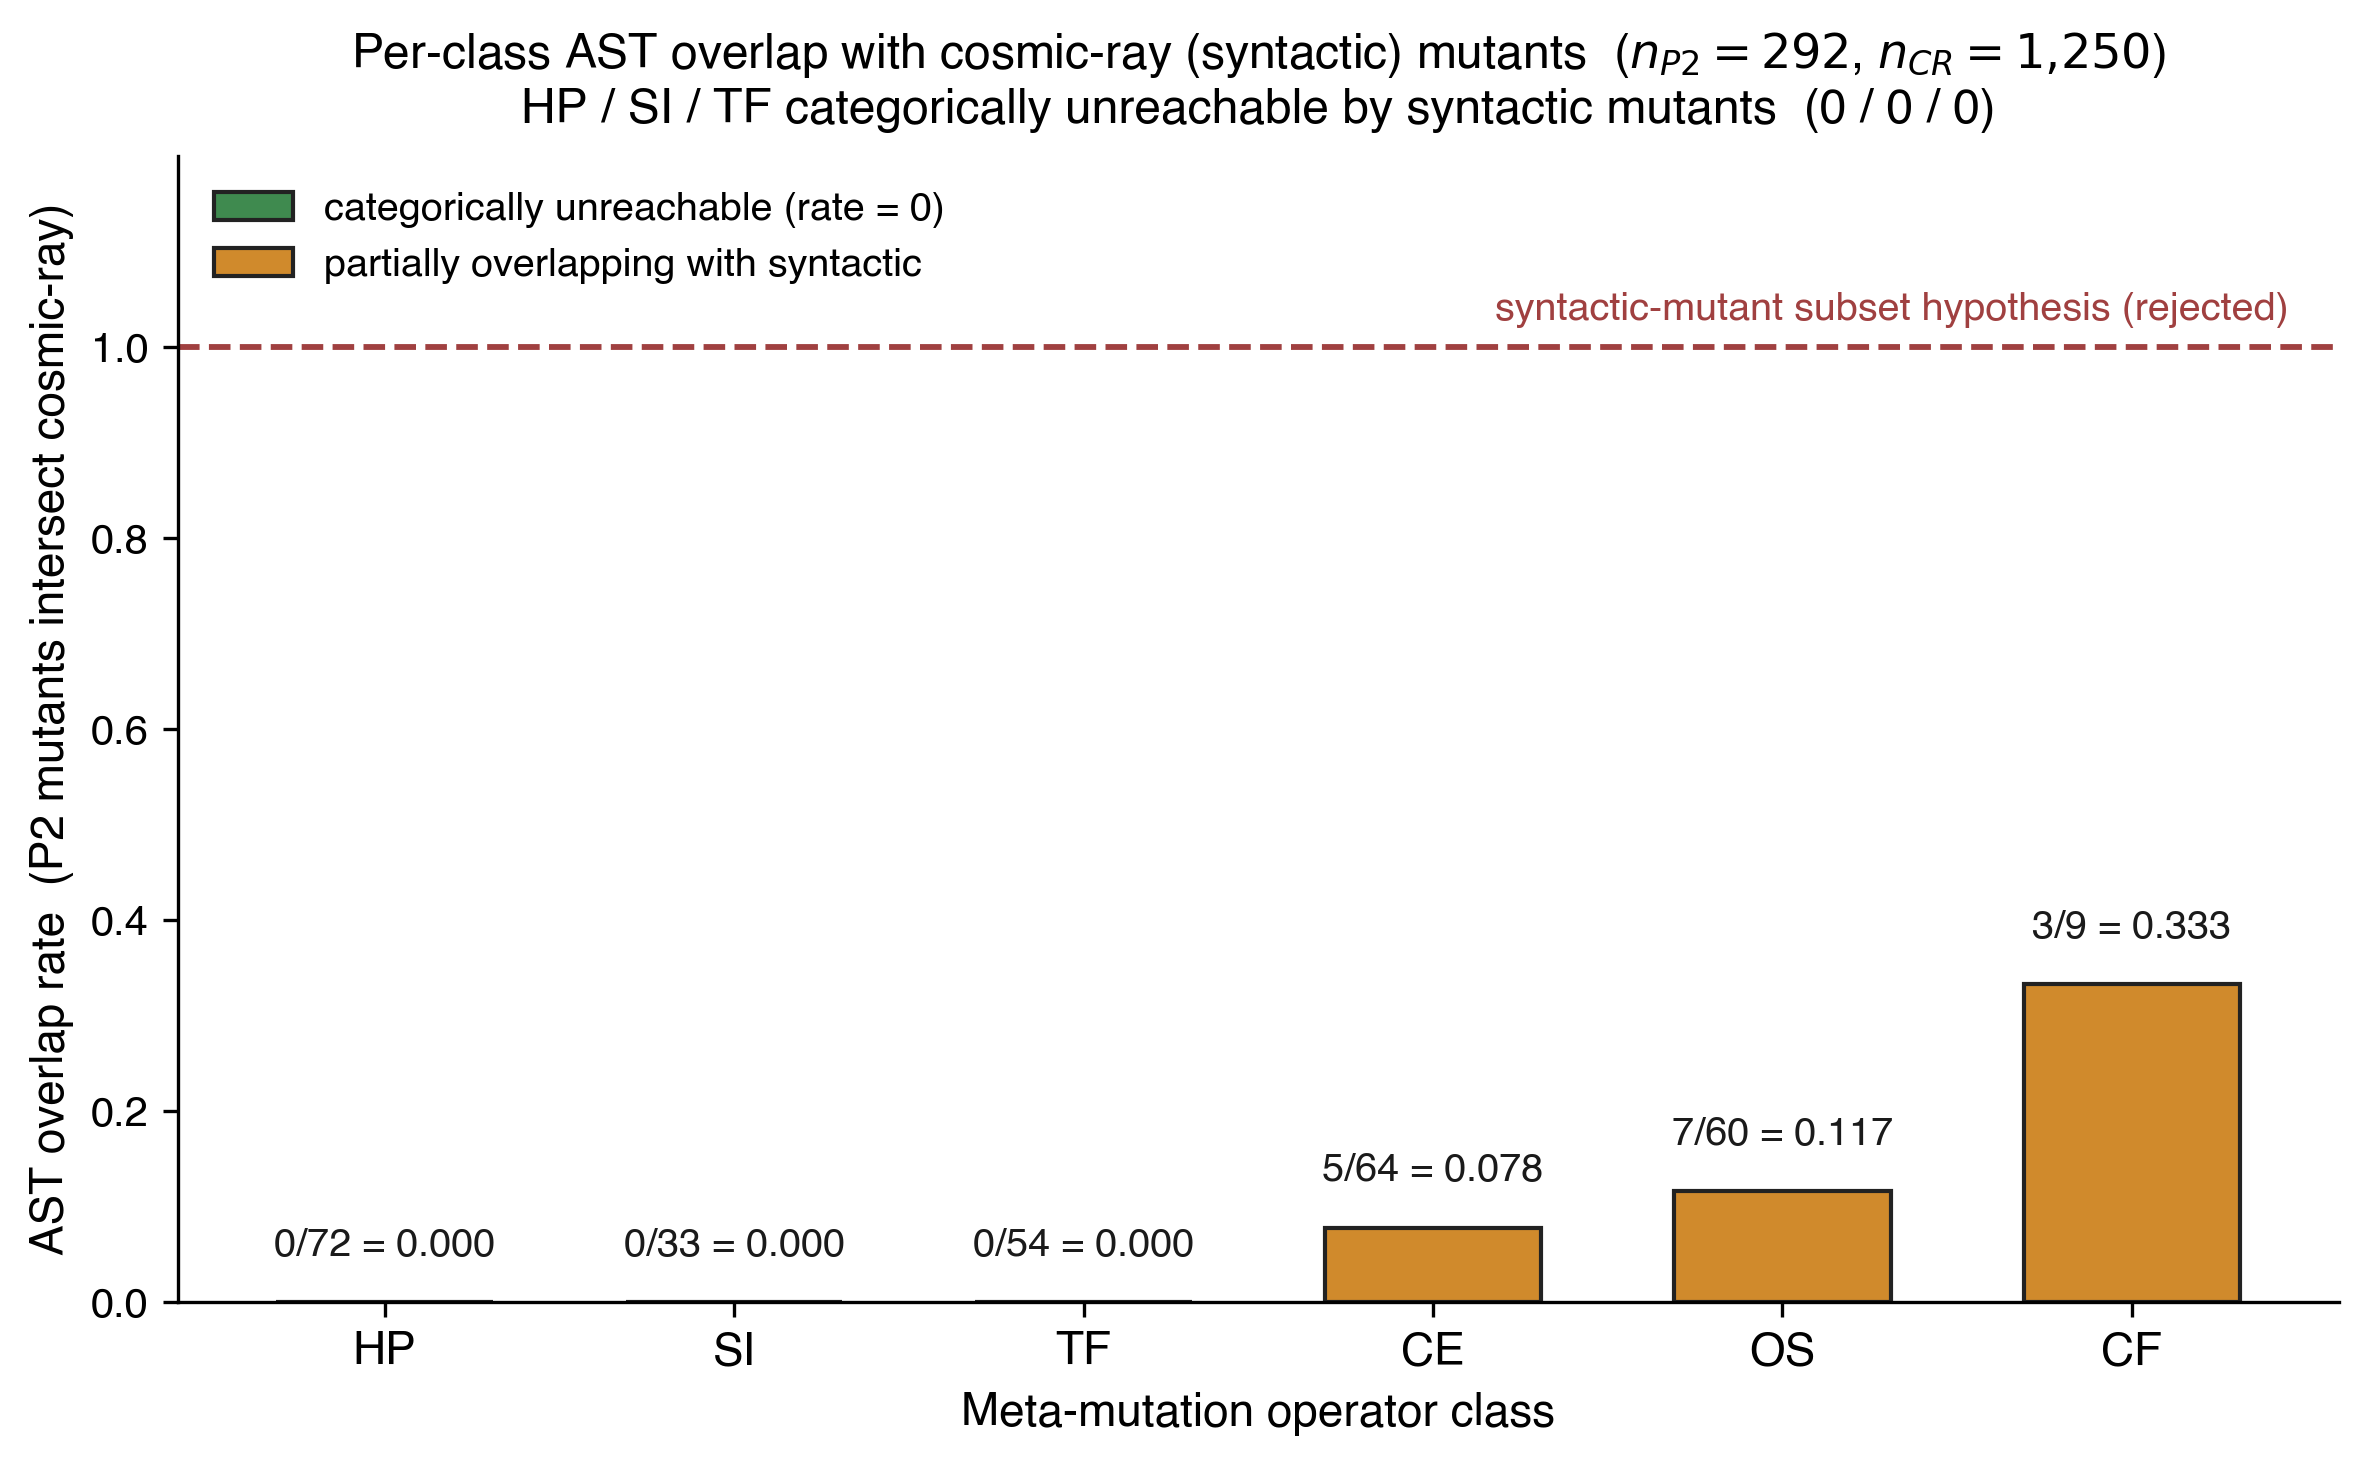
\includegraphics[width=0.48\linewidth,height=0.26\textheight,keepaspectratio,alt={Per-class AST overlap rate between 292 semantic mutants and 1,250 cosmic-ray syntactic mutants across 12 PUTs (overall 5.14\%). HP, SI, TF (54.5\% of the semantic pool) show zero overlap (0/72, 0/33, 0/54); CE 7.81\%, OS 11.67\%, CF 33.33\% (CF is a class-specialisation, not in main 5).}]{figures/png/fig3_ast_overlap_per_class.png}
\caption{Per-class AST overlap rate between 292 semantic mutants and 1,250
cosmic-ray syntactic mutants across 12 PUTs (overall 5.14\%). HP, SI, TF
(54.5\% of the semantic pool) show zero overlap (0/72, 0/33, 0/54): SI and TF
are structurally cross-function, while HP zero overlap reflects the
default first-order value menu; CE
7.81\%, OS 11.67\%, CF 33.33\% (CF is a class-specialisation, not in
main 5).}\label{fig:overlap}
\end{figure}

\subsection{Abstract-Syntax-Tree Overlap against Syntactic Mutants}\label{p2-vs-syntactic-mutants-12-put-empirical-layer-3}

\textbf{Experimental design.} For each PUT, semantic cross-source mutants
(\texttt{data/mutants/\$\{PUT\}\_pool\_v4/}, 292 total) are compared at
the AST-normalised level
(\texttt{ast.dump(annotate\_fields=False,\ include\_attributes=False)})
with cosmic-ray default-operator mutants (1,250 total;
\texttt{scripts/p2\_vs\_syntactic\_ast\_diff\_batch.py}). Source:
\texttt{data/results/cosmic\_ray\_12put\_ast\_diff.json}.

\textbf{Aggregate results.}

{\def\LTcaptype{table} % do not increment counter
\begin{longtable}[]{@{}lllll@{}}
\caption{Semantic vs syntactic mutants, 12-PUT empirical: per-operator-class AST
overlap. Aggregate over 12 PUTs: 292 semantic mutants vs 1,250 cosmic-ray
syntactic mutants, AST-normalised overlap 15, \textbf{overall rate
5.14\%}.}\label{tab:p2-05}\\
\toprule\noalign{}
Class & n\_p2 & n\_overlap & Rate & Interpretation \\
\midrule\noalign{}
\endfirsthead
\endhead
\bottomrule\noalign{}
\endlastfoot
\textbf{HP} & 72 & 0 & \textbf{0.000} & Value-menu artifact (not structural) \\
\textbf{SI} & 33 & 0 & \textbf{0.000} & Structurally cross-function \\
\textbf{TF} & 54 & 0 & \textbf{0.000} & Structurally cross-function \\
CE & 64 & 5 & 0.078 & Boundary class (Section~\ref{necessary-conditions-for-semantic-mutation-layer-1} partial (b)) \\
OS & 60 & 7 & 0.117 & Partial incidental hits \\
CF & 9 & 3 & 0.333 & b2 only, n=9 \\
\textbf{All} & \textbf{292} & \textbf{15} & \textbf{0.0514} & 94.86\% AST-disjoint \\
\end{longtable}
}

\textbf{Interpretation: refuting the ``post-classification copy'' challenge.}
HP, SI, and TF (159 of 292 = 54.5\% of v4 mutants) show \textbf{zero overlap}
with cosmic-ray's default AST-local operators: for SI and TF the gap is
structural (cross-function edits no first-order operator expresses), while HP's
zero overlap is a value-menu artifact (a single-literal edit whose replacement
value the default menu does not enumerate), not a structural impossibility, and
whether HOM compositions \citep{jia2008subtle} close it is a residual threat
(Section~\ref{preventive-defence-framing}). CE shows 7.81\% incidental overlap
(mostly half-step perturbations such as \texttt{\_RHO=28.0\ $\to$\ 27.5}), the
remaining 92.19\% AST-disjoint; OS refines an earlier ``tool-inexpressible''
label to 88.33\% disjoint / 11.67\% incidental hits (stochastic byproducts, not
systematic mutation; Section~\ref{preventive-defence-framing}, Appendix B.1.5).
Overall 94.86\% of v4 mutants cannot be reproduced by cosmic-ray defaults, so the
two pools occupy systematically distinct mutant spaces.

A multi-tool cross-comparison was not run because mutpy is incompatible
with Python 3.10+, and mutmut's operator set overlaps strongly with
cosmic-ray's. The DeepSeek, Claude, and GPT contributions to the 15
overlap files are uneven (DeepSeek 11, Claude 4, GPT 0). Appendix B.3
covers the cosmic-ray a1 single-PUT pre-12-PUT pilot, and Appendix F
discusses the LLM-source distributional-shift threat.

\subsection{Higher-Order Mutation Boundary}\label{preventive-defence-framing}

\textbf{Scope of the claim.} The preventive-defence claim below is
conditional on a first-order syntactic baseline; HOM-based syntactic
compositions are an open question and are not refuted by the Section~\ref{p2-vs-syntactic-mutants-12-put-empirical-layer-3}
evidence.

The HP, SI, and TF zero-overlap result, combined with the Section~\ref{necessary-conditions-for-semantic-mutation-layer-1}
necessary-conditions argument, amounts to a \emph{preventive-defence}
argument: semantic mutation operators address a class of fault
hypotheses that lie beyond the reach of default first-order syntactic
configurations (HOM not refuted). Three points sharpen
this framing.

\textbf{(a) Systematic versus incidental.} Satisfying conditions (a),
(b), or (c) is sufficient for a single semantic mutation, but only when
satisfaction reflects design intent, not stochastic byproduct, does it
constitute a \emph{systematic} semantic mutation method. A syntactic
tool that occasionally hits (a) or (c) with its 13 default operators
does so at a non-zero probability, but the hits are not repeatable and
they carry neither of the two engineering goods we want. First,
designing a semantic mutator like OS \texttt{det\ $\to$\ sum(diag)} requires
knowing that these expressions are equivalent on diagonal matrices but
not on general matrices, a deepening of source-code understanding the
syntactic tool does not exhibit. Second, domain-semantic faults, wrong
physical constants, unit conversions, boundary conditions,
hyperparameter semantics, numerical-method order, are not AST-local; the
syntactic-tool design goals (operator typos, off-by-one errors, negation
flips) do not target them. Systematic semantic mutation therefore
requires (a), (b), or (c) to be design intent. Appendix B.1.5 records
this argument in full.

\textbf{(b) HOM caveat.} The Section~\ref{statistical-analysis-and-empirical-results}
empirics did not run a HOM comparison, so we confine the ``tool
unreachability'' claim to \emph{first-order} syntactic tools (mutmut and
cosmic-ray default configurations) and list HOM equivalence testing as a
residual threat (Appendix F.2). Whether HOM
\citep{jia2009hom,kintis2018effective} compositions can partially
simulate OS or HP effects is analysed conceptually next.

\textbf{Conceptual analysis of HOM reachability (summary).} Higher-order
mutation (HOM; \citealp{jia2008subtle,jia2009hom,kintis2018effective}) composes
multiple first-order operators on one source location. Analysed condition by
condition (full argument in supplementary Appendix K.3), default-operator HOM
cannot systematically reach any of the three necessary conditions: (a)
cross-boundary swaps like \texttt{det(M)\ $\to$\ sum(np.diag(M))} presuppose a
domain-specific equivalence no AST-local chain introduces; (b) HOM is unaware of
which constants are load-bearing, whereas HP is parameter-aware by construction;
and (c) algorithmic-class change requires structural rewrites beyond AST-local
edits. We therefore assert that the
Section~\ref{p2-vs-syntactic-mutants-12-put-empirical-layer-3} 0/0/0
unreachability for HP / SI / TF, while strictly empirical only for first-order
configurations, is unlikely to be refuted by default-operator HOM compositions
on combinatorial grounds; a direct empirical HOM falsification remains a
residual threat. A multi-tool cross-comparison (mutmut, mutpy) was not run
(mutpy is incompatible with Python 3.10+, mutmut's operator set overlaps
cosmic-ray's); the aggregate of the two default sets
(\textasciitilde21 first-order AST-local operator classes) collectively fails
all three necessary conditions (cross-reference in Appendix B.6). The 15
overlaps are also LLM-source-skewed (DeepSeek 11/15, Claude 4/15, GPT 0/15;
distributional-shift threat in Appendix F.2), but this does not affect the
categorical argument: the HP / SI / TF result is 0/0/0 across all three sources.

\subsection{Adjoint Extension Subjects}\label{adjoint-extension-arm-subjects}

The adjoint invariant $\psi_6$ (Section~\ref{theory-setting}) is exercised on a separate,
confirmatory set of three third-party linear-operator libraries:
scipy \texttt{LinearOperator} (linear algebra), pylops real-FFT (signal
processing), and jax \texttt{linear\_transpose} (automatic
differentiation), disjoint from the 12 PUTs and the pre-registered
60-cell. Each library carries a real fixed defect in its adjoint code
path as a ground-truth anchor (scipy \#8900, pylops \#292, jax \#6223).
For each, the MR batteries are adj.self (self-adjointness) and adj.dual
(scaled/dual-operator transpose), and the mutant pool mixes
adjoint-breaking mutants (the real defect among them) with semantically
equivalent mutants a strong MR must \emph{not} kill; the real defects are
reproduced in extracted-diff form because the pre-fix releases are
uninstallable on the host (no \texttt{arm64} wheel). The arm is
confirmatory and additive: it does not alter the 60-cell denominator, the
primary-MP convention, or the pre-registered hypotheses. Full subject
specifications and fault mechanisms are in supplementary Appendix H;
results in Section~\ref{rq4-adjoint-extension-arm}.

\subsection{Empirical Study Procedure}\label{procedure-overview}

With the subjects, operators, and the adjoint extension arm fixed
(Sections~\ref{put-selection-12-puts-4-classes}--\ref{adjoint-extension-arm-subjects}), we now specify the procedure that produces each cell's
measurements.

\noindent\textsf{\small Pipeline order: Section~\ref{put-selection-12-puts-4-classes} PUTs $\to$ Section~\ref{cross-source-v4-protocol-summary} Mutant generation $\to$ LRCA L0 prescreen $\to$ Section~\ref{lrca-three-layer-diagnosis} Equivalence ($E_1 \wedge E_2$) $\to$ AVP $\to$ killed/survive $\to$ LRCA three-layer diagnosis $\to$ SMS + $C_1$\_share report.}

Each (i, k, j) cell is reported with \texttt{inst\_count},
\texttt{equiv\_count}, \texttt{killed\_count}, \texttt{survive\_count},
SMS\_\{i,k,j\}, C1\_share\_\{i,k,j\}, suspect\_share\_\{i,k,j\}, and the
three rates \texttt{inst\_rate\ /\ equiv\_rate\ /\ survive\_rate}
corresponding to RQ3.

\subsection{Cross-Source Generation Protocol}\label{cross-source-v4-protocol-summary}

To isolate the contributions of LLM same-source bias and MR-MP alignment
design to Cliff's delta, we ran a three-stage ablation:

{\def\LTcaptype{table} % do not increment counter
\begin{longtable}[]{@{}
  >{\raggedright\arraybackslash}p{(\linewidth - 6\tabcolsep) * \real{0.2500}}
  >{\raggedright\arraybackslash}p{(\linewidth - 6\tabcolsep) * \real{0.2500}}
  >{\raggedright\arraybackslash}p{(\linewidth - 6\tabcolsep) * \real{0.2500}}
  >{\raggedright\arraybackslash}p{(\linewidth - 6\tabcolsep) * \real{0.2500}}@{}}
\caption{Cross-source protocol.}\label{tab:p2-06}\\
\toprule\noalign{}
\begin{minipage}[b]{\linewidth}\raggedright
Version
\end{minipage} & \begin{minipage}[b]{\linewidth}\raggedright
Mutant pool
\end{minipage} & \begin{minipage}[b]{\linewidth}\raggedright
c-class primary MP
\end{minipage} & \begin{minipage}[b]{\linewidth}\raggedright
Use
\end{minipage} \\
\midrule\noalign{}
\endhead
\bottomrule\noalign{}
\endlastfoot
\textbf{v3} & Same-source (Claude Opus 4.6) & partial-order (pre-registered) & H2
baseline (pre-registered primary) \\
\textbf{v4} & \textbf{Cross-source} (Claude Opus 4.6 + GPT-5.4 +
DeepSeek chat) & partial-order (held at pre-registered) & Isolate LLM-source
diversity \\
\end{longtable}
}

The v4 protocol (\texttt{scripts/cross\_source\_campaign.py}) runs each
(PUT, operator) pair on Claude / GPT / DeepSeek with K=3 trials under an
identical prompt template (temperature 0.7, V1-V4 mechanical-validation
gate). Cross-source pool capacity: 37 operators $\times$ 3 sources $\times$ 3 trials =
333 attempts, 89.5\% V1-V4 pass, 298 confirmed mutants distributed nearly
equally (Claude 101, GPT 98, DeepSeek 99); final-stage rejection of
duplicate and QA-failing mutants leaves the 292 that enter the v4 pool
used for SMS and the AST audit.
Here ``37 operators'' denotes the executable operator-specialisation
inventory: 36 primary PUT-class operator pairs plus one CF
structural-injection specialisation. The conceptual operator family
count remains five (CE, OS, HP, TF, SI); CF is reported only as a
specialised SI/structural-injection row in the AST-overlap audit.

\textbf{Declared confound: protocol asymmetry.} v3 used the
original Phase-1 dual-blind reviewer protocol (Claude generation +
GPT-5.4 review + DeepSeek arbitration); v4 passes V1-V4 mechanical gates
only and does \textbf{not} invoke a reviewer LLM. A fraction of the v3 $\to$
v4 source-axis contrast may therefore reflect a slight quality shift
rather than LLM-source diversity per se. The follow-up study will rerun
dual-blind on the v4 grid, but at $n \geq 30$ PUTs: a same-$n$ rerun
removes the protocol-asymmetry confound yet, at $n = 12$ PUTs, the
$\Delta\delta$ CI remains $\approx 0.44$ wide, so detecting a
$\Delta\delta = 0.20$ source-diversity effect at 80\% power requires
$\approx 30$ PUTs, and the follow-up is therefore designed at that size.
Full per-LLM token / latency / cost figures,
V1-V4 specifications, and the full differential-prompt protocol are in
\textbf{Appendix C.1}.

\subsection{Mutant-pool prescreen and equivalence detection}\label{mutant-pool-prescreen-and-equivalence-detection}

\textbf{Pool prescreen (LRCA L0).} Each candidate passes three gates, static
lint/type checking, a unit self-test for finite output, and a Phase-1
double-blind review sign-off (Claude Opus generator, isolated GPT-5.4 reviewer
emitting a syntactic/executable/fault-injected triple; inconsistent outputs go
to a $\leq 10\%$ manual arbitration queue), with a further 20\% manual re-review
that downgrades the batch if manual--reviewer inconsistency exceeds 10\%. Each
cell produces 30--50 candidates and retains 10--15. The v4 cross-source pool
follows a different L0 path (V1--V4 mechanical validation, duplicate removal, QA
rejection) that does \textbf{not} invoke the reviewer LLM for cost reasons, so v4
C5 (artefact) labels are assigned only at LRCA artefact recheck by a human
reviewer, not inherited from a blind vote; this protocol asymmetry (a possible
v3$\to$v4 quality decline) is declared in
Section~\ref{cross-source-contributes-mutant-quality-not-effect-size}, with full
justification in Appendices C.1--C.3.

\textbf{Equivalence detection (E1 $\wedge$ E2).} For each mutant
$s' \in \mathrm{mut}_j(S_i)$:

\begin{enumerate}
\tightlist
\item
  \textbf{E2 step.} Sample $K_{\mathrm{eq}} = 1000$ inputs
  $x \sim D_S$; compute
  $\|S_i(x) - s'(x)\|$; if $\leq \varepsilon_{\mathrm{eq}}$ for all
  samples, mark E2-pass.
\item
  \textbf{E1 step.} For every $mr \in \mathrm{MR}_{i,k}$, compare
  $\mathrm{AVP}(S_i, mr)$ with $\mathrm{AVP}(s', mr)$;
  if all consistent, mark E1-pass.
\item
  \textbf{Conjunction.} E1 $\wedge$ E2 $\to$ enter $\mathrm{equiv}_{i,k,j}$,
  exclude from SMS denominator. Otherwise pass to AVP-killed
  determination.
\end{enumerate}

E2 is run before E1 because E2 is computationally cheaper (K\_eq scalar
evaluations) and quickly discards numerically distinct mutants; the
remaining candidates are screened by AVP for MR-relation equivalence.
The joint condition is conservative: false-non-equivalent (E1 $\vee$ E2 fail)
is much easier than false-equivalent (both must mis-pass
simultaneously), biasing SMS slightly \emph{low}: truly equivalent mutants misclassified
as non-equivalent remain in the admitted denominator as unkillable
survivors, understating adequacy, an explicit
conservative engineering choice (Appendix A.3).

\textbf{Killed determination.} With OR-aggregation across mr in
MR\_\{i,k\}:

\[
\begin{aligned}
\mathrm{killed}(s', \mathrm{MR}_{i,k}) \iff{} & \exists\,mr \in \mathrm{MR}_{i,k}: \\
& \mathrm{AVP}(S_i, mr) = \text{pass} \wedge
  \mathrm{AVP}(s', mr) = \text{fail}.
\end{aligned}
\]

Each (i, k, j) cell is sampled N = 20 times (statistical replicate) to
compute the per-cell SMS, with mutant-level fail ratios feeding the LRCA
L1 decision. The AVP version is pinned by the frozen dependency file and the
embedded source in the replication package; the reproducibility
package carries the complete AVP source so that the package remains
self-consistent under any upstream evolution.

\subsection{Three-Layer Root-Cause Diagnosis}\label{lrca-three-layer-diagnosis}

For each killed mutant the three-layer decision tree of
Section~\ref{lrca-engineering-attribution-layer-descriptive-not-in-sms} applies
in order (L1 tolerance robustness, all classes; L2 OOD triage, C/D; L3
statistical-assumption baseline, B/D; then artefact recheck), under priority
C5 $>$ C4 $>$ C3 $>$ C2 $>$ C1. Threshold calibration over a 9-grid
($\texttt{ood\_band} \in \{0.02, 0.05, 0.10\}$ $\times$
$\texttt{tolerance\_multiplier} \in \{3.0, 10.0, 30.0\}$, repeats 20) lifts H4
from 10/60 to 12/60 cells; the best combination (ood\_band 0.02,
tolerance\_multiplier 3.0) is primary, with default-threshold results as control
(\texttt{lrca\_60cell\_v3.json}). The 12/60 = 20\% ceiling stays far below the
80\% threshold, so H4 is unattainable on this dataset as an intrinsic property
of LLM-mutant pools. Detailed grid, L0--L3 sub-protocols, and pseudocode are in
\textbf{Appendix A.2 + C.4}.

% [thematic break removed]

\section{Results and Discussion}\label{statistical-analysis-and-empirical-results}

The empirical thresholds H1--H4 are stress tests of this particular
semantic-mutant instantiation, not prerequisites for the definition of
SMS. The positive validation target is narrower and more structural:
SMS must preserve the mutation-score denominator, separate
domain-semantic mutants from default first-order syntactic mutants, make
MR adequacy failures diagnosable, and distinguish mutant kill-rate,
semantic-stratum alignment, and real-defect detection. Thus the failed
thresholds below are reported as boundary findings about operator
applicability, MR design, and kill attribution; they do not invalidate
the metric construction.

\begin{figure}
\centering
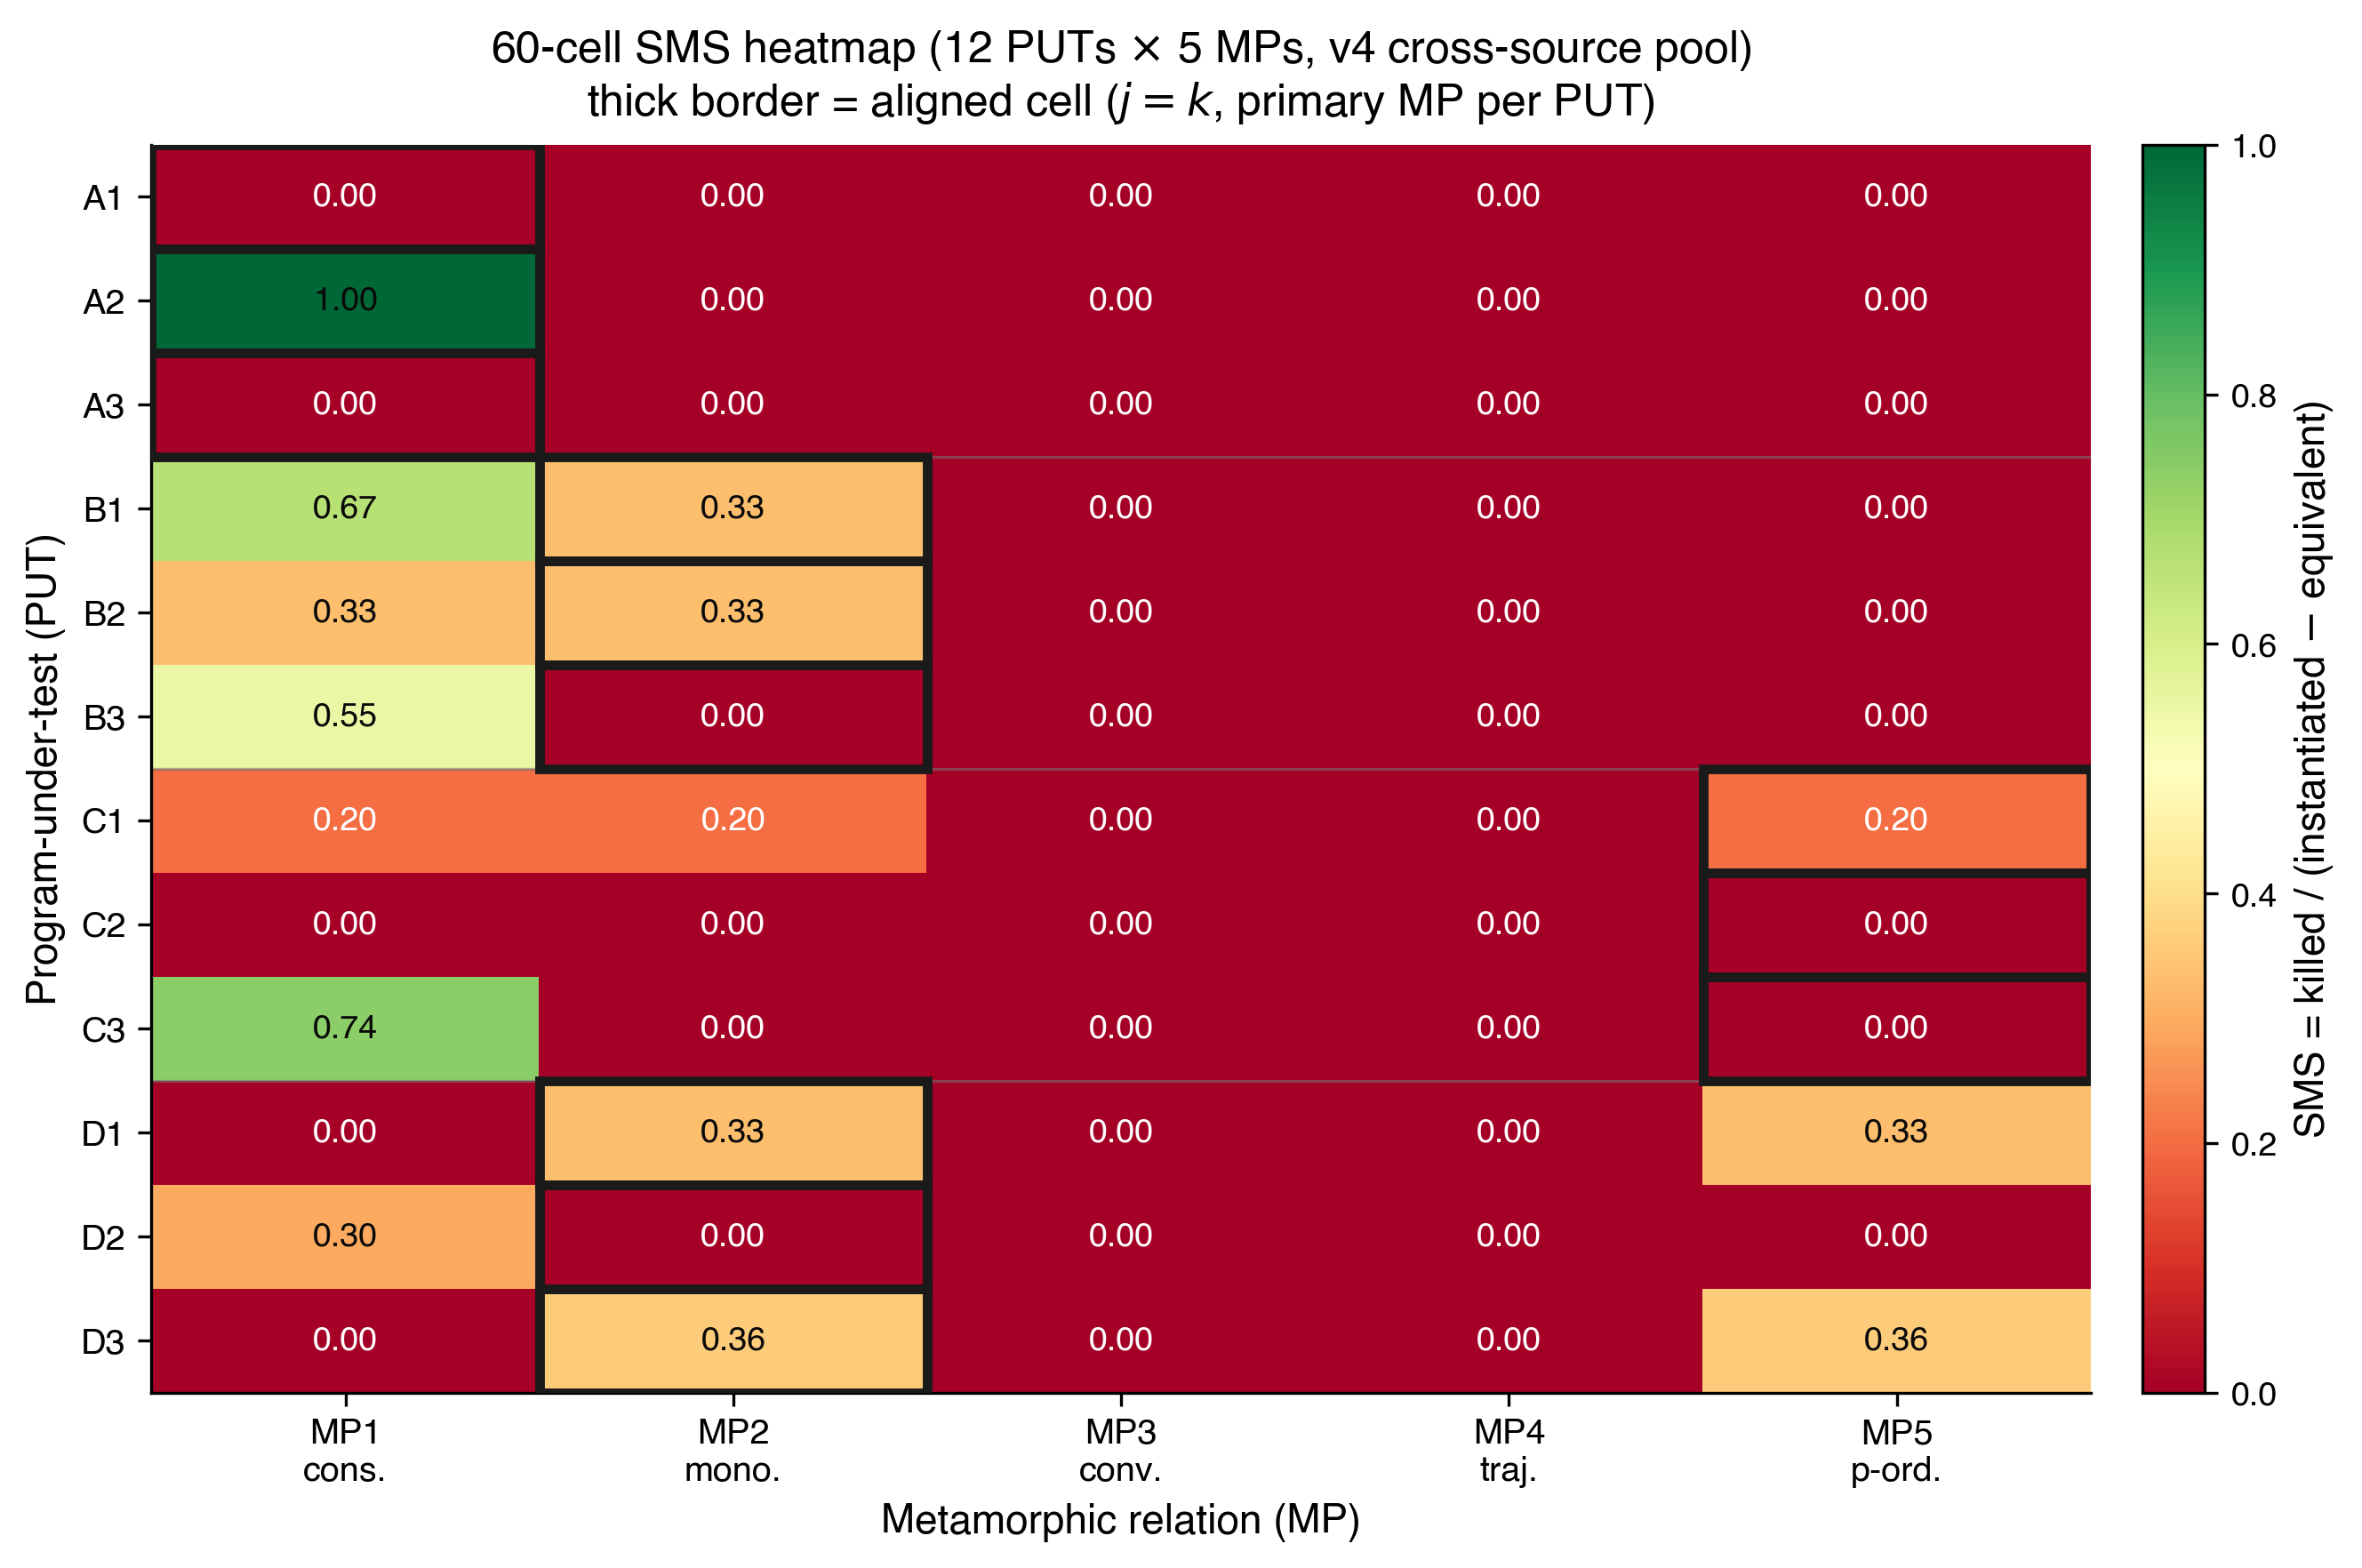
\includegraphics[width=0.48\linewidth,height=0.26\textheight,keepaspectratio,alt={60-cell heatmap of mean SMS over 12 PUTs \textbackslash times 5 MPs (cross-source primary). Diagonal cells (operator-MP aligned) show concentrated mass; off-diagonal mass reflects bleed into adjacent MPs. Empty rows = PUT-level zero-mass cohort (PUTs A1, A3, C2; see Section~\ref{decoupling-between-r_sem-and-r_kill}).}]{figures/png/fig2_60cell_heatmap.png}
\Description{60-cell heatmap of mean SMS over 12 PUTs by five meta-patterns under the cross-source primary pool. Aligned cells concentrate the main signal, while many cross cells are zero; PUTs A1, A3, and C2 form all-zero rows.}
\caption{60-cell heatmap of mean SMS over 12 PUTs \(\times\) 5 MPs (v4
cross-source primary). Diagonal cells (operator-MP aligned) show
concentrated mass; off-diagonal mass reflects bleed into adjacent MPs.
Empty rows = PUT-level zero-mass cohort (PUTs A1, A3, C2; see
Section~\ref{decoupling-between-r_sem-and-r_kill}).}\label{fig:heatmap}
\end{figure}

\subsection{Statistical pipeline}\label{statistical-pipeline}

The primary statistical reporting follows a pre-registered hierarchy:

{\def\LTcaptype{table} % do not increment counter
\begin{longtable}[]{@{}
  >{\raggedright\arraybackslash}p{(\linewidth - 4\tabcolsep) * \real{0.3333}}
  >{\raggedright\arraybackslash}p{(\linewidth - 4\tabcolsep) * \real{0.3333}}
  >{\raggedright\arraybackslash}p{(\linewidth - 4\tabcolsep) * \real{0.3333}}@{}}
\caption{Statistical pipeline.}\label{tab:p2-07}\\
\toprule\noalign{}
\begin{minipage}[b]{\linewidth}\raggedright
RQ
\end{minipage} & \begin{minipage}[b]{\linewidth}\raggedright
Primary statistics
\end{minipage} & \begin{minipage}[b]{\linewidth}\raggedright
Reporting format
\end{minipage} \\
\midrule\noalign{}
\endfirsthead
\endhead
\bottomrule\noalign{}
\endlastfoot
RQ3 & inst\_rate, equiv\_rate, C1\_share, survive\_rate & 60-cell
heatmap + 4-class marginals \\
RQ4 & aligned-SMS vs cross-SMS; sparse $\circ$ vs dense \textbullet\textbullet equiv\_rate &
Cliff's delta + odds ratio + 95\% bootstrap CI \\
RQ5 & $\Delta$SMS\_c (c $\in$ \{A,B,C,D\}); CV($\Delta$SMS) & directional consistency count over the 4 classes (no p-value attached) +
descriptive forest plot \\
RQ5 (desc.) & Spearman $\rho$ + Kendall $\tau$ (SMS vs PC) & scatter + dual-metric ranking
comparison \\
\end{longtable}
}

This pipeline answers the empirical questions RQ3--RQ5; RQ1 is answered
by Theorem~\ref{thm:degeneration} (Section~\ref{sms-ms-degeneration-formal-statement}) and RQ2 by the AST-normalised structural audit
(Section~\ref{p2-vs-syntactic-mutants-12-put-empirical-layer-3}), outside the statistical pipeline.

Where multiple per-class tests are reported (the per-class Friedman tests
of Section~\ref{rq3-cross-class-consistency-and-friedman}), they carry a Bonferroni correction across the four classes; we
do not report a separate cell-level family of p-values, so no family-wise
cell-level correction is claimed. Bootstrap 95\% CIs use 1,000 iterations
as default (B = 10,000 for the headline H2 delta CI). Mixed-effects
modelling
(\texttt{sms\ \textasciitilde{}\ C(class)\ *\ C(operator)\ +\ (1\ \textbar{}\ put)})
failed with a Singular matrix at N = 60: the class $\times$ operator
interaction design matrix is rank-deficient and the PUT random-intercept
variance collapses to the boundary at this sample size. The Friedman test
is the non-parametric formal alternative. The four hypotheses are
pre-registered: H1 (operator implementability) requires $\geq$ 4 of 5
operators producing $\geq$ 5 non-equivalent mutants on $\geq$ 9/12 PUTs; H2
(aligned-vs-cross) requires odds ratio $\geq$ 3.0 \emph{and} Cliff's delta $\geq$
0.474 (Romano 2006 large-effect threshold); H3 (cross-class consistency)
requires sign-test 4/4 across 4 classes plus CV($\Delta$SMS) \textless{} 0.5;
H4 (LRCA mass) requires mean suspect\_share $\leq$ 0.20. SMS variants
(SMS, SMS\_unfiltered) and construction lemmas are in
\textbf{Appendix D.1}.

The results are reported in RQ order. RQ3 is answered in
Section~\ref{rq1-60-cell-distribution}. RQ4 spans the aligned-versus-cross
comparison (Section~\ref{rq2-aligned-vs-cross-cliffs-delta}), its power
analysis (Section~\ref{rq2-stipulated-alternative-power}), the root-cause
diagnostics (Section~\ref{h5-lrca-mass}), the strong-boundary and adjoint
studies (Sections~\ref{rq4-strong-boundary} and~\ref{rq4-adjoint-extension-arm}),
the cross-source analysis
(Sections~\ref{cross-source-contributes-mutant-quality-not-effect-size}
and~\ref{decoupling-between-r_sem-and-r_kill}), and the industrial
construct-separation arm
(Section~\ref{rq4-industrial-construct-separation}). RQ5 follows in
Sections~\ref{rq3-cross-class-consistency-and-friedman}
and~\ref{rq4-sms-vs-pattern-coverage}, with the class-level stability
discussion in Section~\ref{h4-partial-across-same-source-and-cross-source}.

Because the 60 cells share 12 PUTs and are not independent, each reported
statistic carries an explicit inference permission; no number in this paper
should be read above its row. Table~\ref{tab:inference-permissions} is the
single cross-study verdict-and-permission ledger: it lists every hypothesis
across the four studies with its pre-registration status, sampling unit,
verdict, and licensed reading, and \emph{subsumes} the per-study scoreboards
(the Study-2, Study-3, and Study-4 key statistics are reported in the prose of
Sections~\ref{study2-scoreboard}, \ref{study3-scoreboard},
and~\ref{study4-scoreboard}).

{\def\LTcaptype{table} % do not increment counter
\scriptsize
\begin{longtable}[]{@{}
  >{\raggedright\arraybackslash}p{(\linewidth - 8\tabcolsep) * \real{0.26}}
  >{\raggedright\arraybackslash}p{(\linewidth - 8\tabcolsep) * \real{0.19}}
  >{\raggedright\arraybackslash}p{(\linewidth - 8\tabcolsep) * \real{0.15}}
  >{\raggedright\arraybackslash}p{(\linewidth - 8\tabcolsep) * \real{0.12}}
  >{\raggedright\arraybackslash}p{(\linewidth - 8\tabcolsep) * \real{0.28}}@{}}
\caption{Cross-study inference-permission and verdict ledger (all 14 hypotheses
plus the descriptive statistics), spanning Studies 1--4. This
table subsumes the per-study scoreboards.}\label{tab:inference-permissions}\\
\toprule\noalign{}
Statistic & Pre-registration status & Sampling unit (n) & Verdict & Licensed reading \\
\midrule\noalign{}
\endfirsthead
\endhead
\bottomrule\noalign{}
\endlastfoot
H1 operator--PUT counts (S1) & pre-registered threshold & PUT $\times$
operator & NOT MET & deterministic count; verdict factual on this pool \\
H2 Cliff's $\delta$, odds ratio, bootstrap CI (S1) & pre-registered
exploratory large-effect target & cell (12 aligned vs 48 cross;
non-independent within PUT) & NOT MET & point-estimate verdict only; no
population claim (pass probability $\approx$ 0.5 at the boundary is
rule-intrinsic; Section~\ref{rq2-stipulated-alternative-power}) \\
H3 sign test, CV($\Delta$SMS) (S1) & pre-registered threshold & class (n = 4)
& NOT MET & verdict factual on these four classes \\
H4 mean suspect\_share (S1) & pre-registered threshold & cell (n = 60) &
NOT MET & descriptive mean; no independence assumed \\
Friedman $\chi^2$ (MP effect; per-class Bonferroni) (S1) & exploratory
inferential & PUT blocks (n = 12) & sig.\ (expl.) & non-parametric alternative after
mixed-effects singularity; exploratory \\
Spearman $\rho$ / Kendall $\tau$ (SMS vs PC) (S1) & none (descriptive) & PUT
(n = 12) & descriptive & hypothesis-generating only \\
Industrial arm: four-group Wilcoxon, Holm-corrected & pre-registered in
the dataset protocol & case (n = 34, paired) & T1$>$B1 holds & inferential within the
34-case pool; no corpus-level claim \\
Industrial arm: 34/34 real-defect face & none (descriptive; selection-conditioned) & case &
34/34 & face-level count; not a coverage rate \\
H2-1\('\) Cliff's $\delta$ (S2) & pre-registered confirmatory (Family A) &
cell (28 aligned vs 112 cross; non-independent within PUT) & CONFIRM & one-sided
lower bound $>0$ licenses directional dominance; Romano band descriptive
only \\
H1\('\) family counts (S2) & pre-registered confirmatory (Family E) &
PUT $\times$ family & CONFIRM & deterministic count; verdict factual on this pool \\
H3\('\) class direction (S2) & pre-registered confirmatory (Family E) &
class (n = 4) & CONFIRM & direction count; verdict factual on these four classes \\
H4\('\) mean suspect\_share (S2) & pre-registered confirmatory (Family E) &
cell (n = 140) & NOT\_CONF. & descriptive mean; verdict factual (threshold not met) \\
H2-2 cross-vendor $\Delta\delta$ (S2) & registered, gated (Family B) &
n/a (not run) & NOT-RUN & not-run under same-vendor freeze; cross-vendor question
open, not a null \\
H4\('' \)-graded rich-class mean share (S3) & pre-registered confirmatory
(Family G, Holm 2) & detected mutant, aggregated over rich C/D PUTs
($n_{\mathrm{rich}} = 6$) & NOT\_CONF. & one-sided lower bound $\leq 0.15$; verdict factual
(NOT\_CONFIRMED); no purity claim on rich classes \\
H4\('' \)-strict single-stratum purity (S3) & pre-registered confirmatory
(Family G, Holm 2) & detected clean-family mutant ($n = 90$) & CONFIRM & one-sided lower
CP bound $\geq 0.90$ licenses single-stratum validity on \{CE, HP,
CF-with-screen\} only \\
H2-2 cross-vendor $\Delta\delta$ (S4) & pre-registered confirmatory (Family B,
three-way rule) & PUT pairs ($n = 28$, arms paired) & BOUNDED\_NULL & no
source-diversity effect of magnitude $\geq 0.20$ under matched protocol; not
an exact-zero claim \\
H4\('''\)-graded pooled rich-class mean share (S4) & pre-registered
confirmatory (Family H, recruitment-gated) & rich PUT-arm unit
($n_{\mathrm{rich}} = 32$, pooled) & CONFIRM & graded, dominant-but-co-firing
attribution at adequate $n$; never a purity claim; class C alone below the
bar; coupled attribution per sensitivities S1/S2 \\
H-LANG $\delta_C$ (S4) & pre-registered confirmatory (Family L; power 0.6865
disclosed) & C cell (7 aligned vs 28 cross; $n = 7$ PUTs) &
NOT\_CONF. & language-invariance direction does not replicate; the positive
point estimate carries no confirmatory weight \\
\end{longtable}
\normalsize}

\subsection{RQ3: Semantic-Mutation Score Distribution}\label{rq1-60-cell-distribution}

{\def\LTcaptype{table} % do not increment counter
\begin{longtable}[]{@{}ll@{}}
\caption{RQ3: Semantic-mutation score distribution.}\\
\toprule\noalign{}
Metric & Value \\
\midrule\noalign{}
\endhead
\bottomrule\noalign{}
\endlastfoot
Number of cells & 60 \\
Mean SMS & 0.104 \\
Median SMS & 0.000 \\
Std SMS & 0.213 \\
Cells with SMS = 0 & 45 / 60 \\
Mean mutants / PUT (v4) & 24.3 (range 10-30) \\
\end{longtable}
}

The \textbf{zero-mass dominance} (45/60 = 75\%) is concentrated in the
cross-MP slice: \textasciitilde88\% (42/48) of cross cells are zero,
\textasciitilde25\% (3/12) of aligned cells are zero. Cliff's delta is
well-defined under this distribution but its inference is effectively
dominated by
\texttt{n\_aligned\_nonzero\ $\approx$\ 6\ +\ n\_cross\_nonzero\ $\approx$\ 9\ =\ 15}, not the
surface n=60. Three odds-ratio-like quantities must be kept distinct.
First, the pre-registered \emph{median} odds ratio is formally $+\infty$
because the cross-slice median SMS is exactly 0; it degenerates under
zero-inflation and licenses no verdict, so we report ``aligned median
\textgreater{} 0 = cross median'' only as auxiliary qualitative evidence.
Second, a post-hoc \emph{detection-incidence} sensitivity, declared in
its own single-test family (outside the pre-registered Holm family and
outside the H2 pre-registration), binarizes SMS and asks how often each
slice scores any nonzero effect. Under the MP5-held primary convention,
aligned cells are nonzero in 6/12 cases versus cross cells in 9/48
(incidence 50\% vs 18.75\%; only 9 of the 12 PUTs carry any nonzero
cell). A one-sided Fisher exact test gives $p = 0.035$ with
conditional-MLE odds ratio 4.2 (sample OR 4.33; exact one-sided 95\% CI
$[1.12, +\infty)$), and the advantage is directionally stable across
pool variants (OR 4.1--7.0, one-sided $p = 0.006$--$0.049$). Aligned
meta-patterns therefore detect a nonzero effect appreciably more often
than cross patterns, a distinct and modest incidence separation, not the
near-twentyfold ratio that a PUT-level any-signal count (9 of 12 PUTs
non-dead) would suggest if mislabelled as an aligned-cell count. Third,
the Cliff's $\delta$ \emph{magnitude} estimand
(Section~\ref{rq2-aligned-vs-cross-cliffs-delta}) is the pre-registered
H2 criterion: incidence separates, magnitude does not, and the H2
verdict remains \textbf{not met}.

\textbf{Effective-n note.} The surface $n_{\mathrm{aligned}} = 12$,
$n_{\mathrm{cross}} = 48$ mask a much smaller information content: only about 15
observations carry nonzero SMS (6 aligned + 9 cross). This heuristic count (not a
formal effective sample size) explains the wide 95\% bootstrap CI
{[}0.014, 0.622{]} of the v4 primary delta, consistent with the liberal tendency
of the percentile bootstrap when few observations carry signal. Power and
effect-size disambiguation are treated jointly with the stipulated-alternative
analysis in Section~\ref{rq2-stipulated-alternative-power}, and PUT-class
diversification at $n \geq 30$ is a testable route to relaxing the constraint.

\textbf{H1 verdict: not met.} H1 (RQ3) requires at least 4 of the 5
operators to produce $\geq 5$ non-equivalent (confirmed) mutants on at
least 9 of the 12 PUTs. Table~\ref{tab:p2-32} counts confirmed
non-equivalent mutants per operator class across the 12 PUTs: only the
Hyperparameter operator clears the $\geq 9/12$ bar.

{\def\LTcaptype{table} % do not increment counter
\begin{longtable}[]{@{}ll@{}}
\caption{H1: PUTs reaching $\geq 5$ non-equivalent mutants, per operator
class.}\label{tab:p2-32}\\
\toprule\noalign{}
Operator class & PUTs with $\geq 5$ non-equiv mutants (of 12) \\
\midrule\noalign{}
\endfirsthead
\endhead
\bottomrule\noalign{}
\endlastfoot
Conservation Erosion (CE) & 4 / 12 \\
Operator Substitution (OS) & 5 / 12 \\
Hyperparameter (HP) & \textbf{9 / 12} \\
Trajectory Flip (TF) & 5 / 12 \\
Structural Injection (SI) & 1 / 12 \\
\end{longtable}
}

Because the semantic operators are class-targeted, each is applicable to a
subset of the four classes, not uniformly to all twelve; only Hyperparameter
clears the 9-PUT threshold, so 1 of 5 meets the criterion and \textbf{H1 is not
met as pre-registered}, the uniform-applicability assumption behind the
$\geq 9/12$ bar failing for class-targeted operators. A secondary
applicability-adjusted denominator (counting only PUTs with a class-specific
specialisation, Appendix B.2/C.4) gives CE 4/8, OS 5/7, HP 9/9, TF 5/6, SI 1/6,
which does not overturn the verdict but locates its source: HP and TF are
implementable across their intended classes, OS is moderately broad, and SI
remains a narrow high-risk family (per-operator profile in Appendix C.4).

\subsection{RQ4: Aligned and Cross-Pattern Comparisons}\label{rq2-aligned-vs-cross-cliffs-delta}

{\def\LTcaptype{table} % do not increment counter
\begin{longtable}[]{@{}llll@{}}
\caption{RQ4: Aligned and cross-pattern comparisons.}\label{tab:p2-09}\\
\toprule\noalign{}
Slice & n & Mean SMS & Median SMS \\
\midrule\noalign{}
\endhead
\bottomrule\noalign{}
\endlastfoot
aligned (j = k) & 12 & 0.213 & 0.100 \\
cross (j $\neq$ k) & 48 & 0.077 & 0.000 \\
\end{longtable}
}

The means and medians above are those of the MP5-held cross-source pool
(\texttt{rq2\_cliffs\_delta\_v4\_mp5.json}) that generates the headline
$\delta = 0.314$ reported below, so the summary statistics and the effect
size share one provenance. (The unconditioned v4 pool with the c-class
primary at MP1 gives higher means 0.275 / 0.061 and $\delta = 0.439$; the
power analysis in Section~\ref{rq2-stipulated-alternative-power} is run on
that unconditioned pool, as noted there.)

Two delta point-estimates under the pre-registered primary-MP
convention:

\begin{itemize}
\tightlist
\item
  \textbf{v3 (same-source, pre-registered):} delta = \textbf{0.323},
  95\% CI {[}0.017, 0.622{]}
\item
  \textbf{v4 (cross-source, c-class held at partial-order):} delta =
  \textbf{0.314}, 95\% CI {[}0.014, 0.622{]}. The cross-source pool
  aggregates Claude / GPT / DeepSeek under an identical prompt; the
  c-class primary is held at the pre-registered partial-order
  meta-pattern so that the v3 $\to$ v4
  contrast holds the prompt and primary-MP choice fixed. Because v4 uses
  mechanical gates rather than the v3 dual-blind reviewer step, the
  source-axis reading is qualified by the protocol-asymmetry analysis in
  Section~\ref{r13-protocol-asymmetry-magnitude-estimate}.
\end{itemize}

\textbf{H2 verdict: not met.} H2 carries two pre-registered criteria,
Cliff's $\delta \geq 0.474$ and an aligned-to-cross odds ratio
$\geq 3.0$. Neither delta crosses the \citet{romano2006cliff}
large-effect threshold 0.474, 0.323 and 0.314 both fall just below the
\citet{romano2006cliff} medium threshold of 0.330, so the delta criterion fails. The
Romano threshold is retained as the frozen decision anchor because it is
the threshold recorded in the experiment design; we do not re-anchor the
verdict post hoc to a Vargha--Delaney interpretation scale. The
odds ratio is degenerate: because the cross-slice median SMS is exactly
0 (table above), the median odds ratio is $+\infty$, so the ratio
criterion is satisfied only trivially under zero-inflation and carries no
evidential weight. H2 is therefore not met as a large-effect target. The
contrast $\delta_{\mathrm{v4}} - \delta_{\mathrm{v3}} = -0.009$ (paired-role
bootstrap 95\% CI {[}-0.238, 0.207{]}) is too small to interpret as a stable LLM-source-diversity effect
under the present asymmetric protocol: replacing a same-source pool with
a three-LLM cross-source pool does not appreciably shift Cliff's delta
within this design, but the exact source-diversity contribution requires
a dual-blind v4 rerun. We frame H2 as an underpowered exploratory
contribution and defer full verification to a follow-up study with a
larger PUT sample.

\textbf{Vacant-cell sensitivity.} Excluding the 9 cells marked vacant in
Table~\ref{tab:p2-cells} gives the same H2 verdict. Under the frozen
primary-MR convention, v4 has n = 11 aligned and n = 40 cross cells,
$\delta = 0.323$ with 95\% CI {[}-0.011, 0.648{]}; v3 has
$\delta = 0.270$ with 95\% CI {[}-0.043, 0.595{]}. The direction remains
positive but still below 0.474, and the interval crosses zero once vacant
cells are removed. The sensitivity is a denominator check, not a changed
conclusion.

This medium-effect placement is consistent with \citet{tip2025llmorpheus}
LLMorpheus's medium-effect range on JavaScript LLM mutants, a contextual
literature observation (estimand caveat: their delta compares ``LLM vs
traditional mutants on fault detection'', ours compares ``aligned vs
cross MP slice within one pool''; the numerical similarity is not
substantive support).

\subsection{RQ4: Stipulated-Alternative Power Analysis}\label{rq2-stipulated-alternative-power}

The Section~\ref{rq1-60-cell-distribution} effective-n constraint motivates an
explicit power analysis (full exceedance and stipulated-alternative tables in
supplementary Appendix K.4; sample-size sweep in Appendix D.3). A plug-in
bootstrap (5,000 replications, seed 42) over the unconditioned
($n=12$, $n=48$) pool ($\delta = 0.439$) exceeds the ``any effect''
threshold with probability 0.997, the medium threshold (0.330) with 0.759, and
the large H2 threshold (0.474) with only 0.423. A stipulated-alternative
simulation, in which the truth is fixed at the H2 boundary 0.474 (a mixture
calibrated to $E[\delta] = 0.4746$, since SMS ties at zero make a raw shift
discontinuous), returns the point-estimate pass rule with power \textbf{0.491}
and the ``lower 95\% CI bound $>0$'' rule with power 0.868.

Even when the truth equals the H2 boundary, the point-estimate decision rule
returns ``not met'' in roughly half of replications; a pass probability near
one half at the boundary is intrinsic to a threshold rule applied to an
approximately median-unbiased estimator at any sample size, so the 49.1\%
figure characterises the pre-registered decision rule, not a deficiency
specific to the (12, 48) design. This supports the framing in
Section~\ref{rq2-aligned-vs-cross-cliffs-delta}: the H2 verdict is a factual
statement about the point estimate failing to clear the threshold, not a claim
that the effect is necessarily smaller than 0.474. Increasing the sample size
narrows the confidence interval but cannot lift the point estimate.

\textbf{The source-axis contrast is underpowered too.} We did not run a
separate power simulation for the source-axis contrast $\Delta\delta$ =
−0.009 (paired-role bootstrap 95\% CI {[}-0.238, 0.207{]}); its estimand and dependence structure differ
from the aligned-vs-cross $\delta$, so the 49.1\% figure above does not
transfer to it. The small design (n = 12 PUTs) leaves the −0.009 null
consistent with a wide range of true source-diversity effects, so we
explicitly do not read it as evidence that source diversity is inert. A
properly-powered strong-sense test is deferred to a follow-up study.

\textbf{Note on monotone-transformation invariance.} Cliff's $\delta$ is
rank-based: a function of $U / (n_1 \cdot n_2)$, so applying a logit transform to
SMS gives $\delta_{\mathrm{logit}} \equiv \delta_{\mathrm{raw}}$ by construction. This is consistent with the
rank-invariance theorem and does \textbf{not} constitute additional
robustness evidence. The genuine robustness threats to the H2 verdict
come from the zero-mass dominance (Section~\ref{rq1-60-cell-distribution}), not from any metric-scale
choice.

\subsection{RQ4: Root-Cause Diagnostic Results}\label{h5-lrca-mass}

\begin{table}[t]
\caption{RQ4: Root-cause diagnostic mass.}
\label{tab:p2-13}
\centering
\begin{tabular}{ll}
\toprule
Metric & Value \\
\midrule
Mean C1\_share (v3 same-source pool) & 0.164 \\
Mean C1\_share (v4 cross-source pool) & \textbf{0.209} \\
Mean suspect\_share (v4 cross-source pool) & \textbf{0.791} \\
Cells with suspect\_share $\leq$ 0.20 (secondary; threshold-calibration best, ood\_band = 0.02) & 12 / 60 = 20.0\% \\
\bottomrule
\end{tabular}
\end{table}

\textbf{H4 verdict: not met.} The pre-registered criterion is mean
suspect\_share $\leq$ 0.20; the observed mean is \textbf{0.791} (v4),
decisively above the threshold, so H4 fails on its own metric. A dense
cutoff sweep (Appendix D.2) confirms this is an intrinsic property of
LLM-mutant pools rather than a calibration artefact: the secondary
per-cell pass-ratio (cells with suspect\_share $\leq$ 0.20) is flat at
12 / 60 = 20\% across cutoffs $\in$ {[}0.05, 0.40{]}, because v4's
suspect\_share distribution is severely bimodal (median 1.0, with 48
cross cells near 1 and 12 aligned cells near 0; the {[}0.20, 0.80{]}
interior is nearly empty). H4 was pre-registered before pool
characteristics were known, so this is a finding worth reporting.

\textbf{C1-weighted sensitivity.} Because LRCA deliberately does not
filter SMS, we add a diagnostic secondary view
$\mathrm{SMS}_{\mathrm{C1}} = \mathrm{SMS} \times \mathrm{C1\_share}$.
On the v4 60-cell table, mean SMS is 0.104 and mean
$\mathrm{SMS}_{\mathrm{C1}}$ is 0.0873; nonzero cells fall from 15/60 to
13/60. The conclusion is therefore conservative: suspect mass is high
and H4 is not met, but the main positive SMS signal is not created solely
by suspect labels. We keep raw SMS as the primary metric because LRCA is
a diagnostic attribution layer, not part of the mutation-score
denominator.

\subsection{RQ4: Strong-Boundary Failure Modes}\label{rq4-strong-boundary}

The 60-cell audit (Sections~\ref{rq1-60-cell-distribution}--\ref{h5-lrca-mass}) exercises strong MRs in the regime where
Theorem~\ref{thm:duality} holds. To map the strong boundary of Proposition~\ref{prop:boundary} we run a
complementary study on six third-party or textbook programs spanning the
meta-patterns, kept separate from the 12 PUTs. Wherever a genuine fixed
defect exists in a third-party library we use real version-switching:
the pre-fix and post-fix releases run unmodified in isolated environments,
and we record the repository, the version pair, and the issue/PR, and
we fall back to a textbook faithful implementation only when the real
defect cannot be exercised on the host (no \texttt{arm64} wheel, a
heavyweight Fortran build, or a drift below machine resolution).
$\varepsilon_{\mathrm{tol}}$ is an explicit factor in every case.

{\def\LTcaptype{table} % do not increment counter
\begin{longtable}[]{@{}p{1.6cm}p{3.4cm}p{2.5cm}p{2.6cm}p{1.7cm}@{}}
\caption{RQ4: Strong-boundary map over six programs.}\label{tab:p2-30}\\
\toprule\noalign{}
Family & Program (provenance; method) & Strong MR ($\varepsilon_{\mathrm{tol}}$) & Correct / faulty verdict & Boundary role \\
\midrule\noalign{}
\endfirsthead
\endhead
\bottomrule\noalign{}
\endlastfoot
inv.con & non-conservative Burgers; \citep{hou1994nonconservative} (textbook) & shock speed ($0.03$) & $0.498$ pass / $-0.002$ killed & strong \\
inv.eqv & scipy \texttt{align\_vectors} $1.13.0\to1.13.1$, \#20660 (real) & rotation residual ($10^{-6}$) & $10^{-16}$ pass / $2.0$ killed & strong \\
adj.self & scipy \texttt{\_adjoint} \#8900/PR\#8962 (real, extracted-diff) & adjoint-identity residual & $10^{-16}$ pass / $1.4$--$2.0$ killed & strong \\
rev.traj & leapfrog vs explicit Euler; \citep{hairer2006geometric} (textbook) & energy-drift ratio ($\leq 3$) & $1.00$ pass / $1952$ killed & strong \\
PINN & soft vs hard BC; DeepXDE \#26 (real torch) & exact BC $|u(0)|$ ($10^{-4}$) & hard $0$ pass / soft $5\times10^{-4}$ killed & FP (weak MR) \\
struct.\ (FN) & numpy float32 RNG $1.21.6\to1.22.0$, \#17478 (real) & mean / range / dist & both pass; buggy survives & FN (surviving) \\
\end{longtable}
}

\textbf{Strong regime (four cases).} For inv.con, inv.eqv, adj.self, and
rev.traj the correct program satisfies the strong MR within
$\varepsilon_{\mathrm{tol}}$ while the faulty program is killed, exactly as
Theorem~\ref{thm:duality} predicts. Two are real fixed library defects (scipy
\texttt{align\_vectors}; scipy \texttt{\_ScaledLinearOperator.\_adjoint},
exercised by reverse-applying the fix diff because the pre-fix release has no
\texttt{arm64} wheel); two are textbook contrasts for defects unexerciseable on
the host (Burgers conservative/non-conservative for the GeoClaw conservation
bug; symplectic leapfrog vs explicit Euler for the REBOUND IAS15 drift, real
signature near $10^{-14}$ below resolution).

\textbf{False positive, weak MR (PINN).} A soft-penalty PINN is a legitimately
trained, non-faulty model, yet its exact-boundary residual
$|u(0)| \approx 5\times10^{-4}$ exceeds a strict
$\varepsilon_{\mathrm{tol}} = 10^{-4}$, so the strong MR flags it: the
discretisation (soft constraint), not a fault, breaks the invariant, the
empirical face of Proposition~\ref{prop:boundary}(i). The hard-constraint ansatz
$u = x(1-x)\,\mathrm{NN}(x)$ satisfies the invariant by construction and passes.

\textbf{False negative, surviving non-equivalent mutant (RNG).} The numpy
float32 defect (\#17478) zeroes the lowest mantissa bit; the structural MR
family (mean $\approx 0.5$, range $[0,1)$, distribution shape) is satisfied by
both releases within $\varepsilon_{\mathrm{tol}}$, so the genuinely
non-equivalent buggy version survives (coincidental MR satisfaction; an
odd-bit-fraction discriminator reads $0.0$ for the buggy vs $\approx 0.5$ for the
correct release, so it is non-equivalent, not a classical equivalent mutant).
It is the empirical face of Proposition~\ref{prop:boundary}(ii).

\textbf{The $\varepsilon_{\mathrm{tol}}$ trade-off.} The PINN case makes the
sensitivity--specificity coupling runnable: at strict
$\varepsilon_{\mathrm{tol}} = 10^{-4}$ the soft-BC model is killed (false
positive), at loose $10^{-3}$ it survives, and had the residual arisen from a
true fault, loosening would instead cause a false negative. The strong boundary
is thus a tunable operating point, the honest scope of the duality, not a defect
to remove.

\subsection{RQ4: Adjoint Extension Evidence}\label{rq4-adjoint-extension-arm}

Where Section~\ref{rq4-strong-boundary} maps the boundary at which the duality fails, a small
confirmatory arm checks it holding in the forward direction for the sixth
meta-pattern $\psi_6$. On the three third-party linear-operator libraries
of Section~\ref{adjoint-extension-arm-subjects} (scipy, pylops, jax), each carrying a real fixed adjoint defect, a
strong adjoint MR detects only the active mutants: across all three
substrates the correct program survives, every non-equivalent mutant
(including the three real defects scipy \#8900, pylops \#292, and jax
\#6223) is killed, and no semantically equivalent mutant is killed, giving
a forward SMS of 1.00 with zero false positives on the equivalent set
(full subjects, mutant pools, and the per-substrate kill table in
supplementary Appendix H). The arm is confirmatory and additive, it
does not enter the 60-cell denominator and leaves H1--H4 unchanged, and
carries two scope caveats: the scipy \#8900 defect is shared with the Section~\ref{rq4-strong-boundary}
boundary study (so it is not counted as independent corroboration twice),
and the pools are hand-constructed, low-cardinality sets with the real
defects reproduced in extracted-diff form, so the arm demonstrates rather
than measures adequacy (adjoint-arm reproduction-fidelity threat).

% [thematic break removed]

\phantomsection\label{discussion}

\subsection{Cross-source contributes mutant quality, not effect size}\label{cross-source-contributes-mutant-quality-not-effect-size}

Going from same-source to cross-source under the pre-registered primary-MP
convention shifts Cliff's $\delta$ by only $-0.009$ (95\% CI {[}$-0.238$,
0.207{]}) while raising mean C1\_share from 0.164 to 0.209 (+27\%), class-c mean
SMS by \textbf{+91.5\%}, and class-d by 38.3\%. Within this fixed-prompt design,
LLM source identity is therefore not the dominant factor behind the H2 ceiling:
cross-source pooling improves the diagnostic quality of the kill set without
moving the aligned-vs-cross effect size. This is a scoped null, not a claim that
LLM diversity is inert; the strong-sense test with per-LLM differential prompts
(V\_persona, V\_cot) is deferred (Appendix C.1). The
Section~\ref{p2-vs-syntactic-mutants-12-put-empirical-layer-3} evidence (94.86\%
of v4 mutants AST-disjoint from cosmic-ray defaults; HP/SI/TF at 0/0/0) confirms
the medium-effect ceiling is not an artefact of LLM-pool overlap with the
syntactic space, so a larger aligned-versus-cross effect points first to
MR-design refinement, not more sampling. (As a contextual coincidence,
\citeauthor{petrovic2021improve}'s \citeyearpar{petrovic2021improve}
$\sim$20\% productive-mutant rate at Google is close to our calibration-sweep
C1\_share of 0.20, distinct from the pool values 0.209 (v4) and 0.164 (v3); the
constructs differ (developer survey vs kill-behaviour annotation), so this is
not mechanism validation.)

\subsection{Decoupling between Semantic Feasibility and Kill Rate}\label{decoupling-between-r_sem-and-r_kill}

The operator-level pilot in Appendix C.4.1 reveals a sharp pattern: HP, TF,
and OS operators on the c-class (surrogate) and d-class (ML) PUTs reach
R\_sem $\approx$ 1.0 (a valid, executable, intent-bearing mutant) but
R\_kill = 0 under the PUT's primary MP. Six cells show R\_sem $\geq$ 0.9 with
R\_kill = 0 (e.g.\ c1\_CE1 GPR \texttt{noise\_level} 1e-4 $\to$ 1e-1, c3\_HP1
relu $\to$ tanh, d1\_HP1 MLP $\alpha$ 1e-4 $\to$ 1.0; full list in Appendix C.4.1):
the mutant is a valid injection, but the primary MP (partial-order for the
c-class, monotonicity for the d-class) is an asymptotic or statistical relation
whose tolerated parameter deviation absorbs the mutant. These examples also
expose a family-boundary caveat: activation-swap or iteration-cap edits sit near
the OS/HP and HP/TF boundaries, so the family label records generating intent,
not a unique structural class, and the aligned-versus-cross reading carries this
labelling slack.

\phantomsection\label{s5-audit}
\textbf{S5 stratum-purity audit.} We verified S5 directly rather than
resting on generation intent. Running all five invariant checkers on
each of the 292 admitted mutants (the deterministic offline AVP
dispatcher, 20-repeat majority vote; SSOT \texttt{s5\_purity\_v4.json})
yields the invariant-flip distribution $\{0{:}170,\,1{:}93,\,\ge 2{:}29\}$.
The effect map $\sigma$ is therefore single-valued on 263/292 (90.1\%) of
the corpus; the 29 multi-stratum mutants (9.9\%) are confined to two
operator families that mutate shared upstream state, control-flow
reversal (CF, 9/9) and training-data corruption (TF, 20/54), while the
four local-edit families (CE, OS, HP, SI) are 100\% pure (0/229;
Table~\ref{tab:s5-purity}). Re-attributing the aligned-versus-cross
off-diagonal kill mass, 57/88 (64.8\%) comes from pure single-invariant
mutants (genuine cross-stratum detection) and 31/88 (35.2\%) from
multi-stratum mutants, the latter confined to the five cells
\texttt{B2\_MP1}, \texttt{C1\_MP1}, \texttt{C1\_MP2}, \texttt{D1\_MP5},
and \texttt{D3\_MP5}. The fiber partition thus survives at the $\sigma$
level (R2's $\ge 90\%$-purity decision rule is met), and the
aligned-versus-cross contrast should be read as a 57:31 pure/multi-stratum
split rather than as uniformly pure cross-stratum detection.

{\def\LTcaptype{table} % do not increment counter
\begin{longtable}[]{@{}lrrrr@{}}
\caption{S5 stratum-purity audit of the v4 corpus. ``Detected'' = killed
by at least one MP invariant checker; ``pure'' = killed by exactly one
(S5 holds); ``multi-stratum'' = killed by two or more ($\sigma$
multi-valued). Multi-stratum leakage is confined to CF and TF, which
mutate shared upstream state.}\label{tab:s5-purity}\\
\toprule\noalign{}
Operator & Mutants & Detected & Pure (flip 1) & Multi-stratum ($\ge 2$) \\
\midrule\noalign{}
\endfirsthead
\endhead
\bottomrule\noalign{}
\endlastfoot
CE & 64 & 27 & 27 & 0 \\
OS & 60 & 35 & 35 & 0 \\
HP & 72 & 11 & 11 & 0 \\
SI & 33 & 11 & 11 & 0 \\
CF & 9 & 9 & 0 & 9 \\
TF & 54 & 29 & 9 & 20 \\
\textbf{All} & \textbf{292} & \textbf{122} & \textbf{93} & \textbf{29} \\
\end{longtable}
}

The cell-level evidence (Section~\ref{rq1-60-cell-distribution}) reproduces the
pattern: 75\% of cells are zero, concentrated in the cross slices, while v4
cross-source raises mean C1\_share from 0.164 to 0.209 (+27\%) among the few
kills. Source diversity therefore improves the \emph{quality} of the kill set
without expanding its \emph{coverage}. \textbf{The engineering insight is that
operator-MP alignment in MR design is necessary for strong SMS signals; merely
enlarging the semantically feasible mutant pool dilutes the C1 proportion
without lifting the kill rate.} This motivates the source-axis reading in
Section~\ref{rq2-aligned-vs-cross-cliffs-delta}: the v3 $\to$ v4 micro-shift of
$-0.009$ estimates LLM source diversity under a fixed prompt, while MR-design
adequacy at the operator-MP level governs the kill rate.

\subsection{RQ4: Industrial Construct-Separation Evidence}\label{rq4-industrial-construct-separation}

The industrial arm answers the last clause of RQ4: whether the
construct separation among aggregate kill-rate, semantic alignment, and
real-defect detection remains visible outside synthetic mutants and
outside author-written kernels. The arm is a 34-case study over
reproduced, MR-detectable defects from widely used scientific-computing
libraries, drawn from an archived dataset
\citep{defect4mr2026}
(\href{https://doi.org/10.5281/zenodo.21203424}{10.5281/zenodo.21203424});
each case pairs a buggy and a fixed revision and registers the
metamorphic relation that discriminates the two. We report verified
result totals only, and the arm does not change the
paper into a benchmark article:
defect mining, rejected cases, repository tooling, and benchmark release
are left outside the paper and remain contributions of the dataset. The result-level evidence summary used here is included
in the supplementary evidence package: it records the five-stratum counts,
the aggregate mutation-phase statistics, the 34/34 real-defect face, and
the non-nesting case identifiers, but not candidate mining or tooling. In
the four-group mutation-phase comparison pre-registered in the dataset
protocol, the four groups are the case's registered pattern-derived
relation (T1), literature-generic baseline relations (B1), seeded
random relations (B2), and mechanical ablations of T1 (A1); the
comparison family is three one-sided case-level Wilcoxon signed-rank
comparisons (T1 $>$ B1, T1 $>$ A1, B1 $>$ B2) under Holm correction,
and the case census (n = 34) was fixed by the dataset's verification
status before any comparison was run. Under the primary all-mutant
denominator the group kill rates are T1 377/1124 = 0.335 (Wilson 95\%
CI {[}0.308, 0.364{]}), A1 348/1124 = 0.310, B1 274/1124 = 0.244, and
B2 228/1124 = 0.203. The pattern-derived group beats the
literature-generic baselines (mean paired difference +0.101, bootstrap
95\% CI {[}+0.029, +0.179{]}, Holm-adjusted \(p=0.046\), Cliff's
\(\delta=+0.247\); one-sided Wilcoxon signed-rank \(V = 279.5\),
\(z = 2.16\), unadjusted \(p = 0.015\); case-resampling bootstrap
\(B = 10{,}000\), seed 20260704). Because the Holm-adjusted \(p\) sits
close to the 0.05 boundary, we additionally report distribution-free
checks of the \emph{same} one-sided \(T1 > B1\) contrast (robustness of
the pre-registered estimand, not new hypotheses): an exact sign-flip
permutation test on the signed-rank statistic (full \(2^{27}\)
enumeration over the 27 nonzero paired differences) gives
\(p = 0.014\), a Monte Carlo sign-flip test on the mean paired
difference (\(B = 10{,}000\)) gives \(p = 0.005\), and the BCa bootstrap
95\% CI for Cliff's \(\delta\) (\(B = 10{,}000\)) is
\([+0.07, +0.46]\), excluding zero. The verdict is marginal under the
Holm-adjusted normal approximation but robust under exact inference, and
is reported with its fragility: the paired difference narrowed when the
dataset grew from 30 to 34 cases, and a sensitivity rerun recorded in the dataset report
(excluding the one case with a known tolerance-storm pathology) leaves
the Holm-adjusted verdict unchanged. The other two family members are
not significant after Holm correction: the pattern-derived group does
not significantly dominate its ablations, and the generic baselines do
not significantly dominate the random draws. On the real-defect face, however, the distinction becomes
sharper: the pattern-derived relation detects every real defect in the
reported mutation-suite face (34/34). Because case admission itself
requires an MR-detectable behavioural difference under the registered
pattern-derived relation, this 34/34 count is selection-conditioned
rather than evidential; the informative content of the face lies in the
contrast on the same admitted cases: the literature-generic baselines
detect nothing in 27 of 34 cases, the seeded random relations in 26 of
34, and the dimension-reduction ablation loses the real defect in 19 of
34 cases that its parent relation detects; a second, de-strictification
ablation loses it in 17 of 34, with 11 cases lost by both (supplementary
Appendix I).

The arm's cases were selected by a fixed inclusion rule: a case had to have a
verified semantic fault, an executable pre/post or faithful contrast, and
an MR-detectable behavioral difference under the declared stratum.
Cases requiring unsupported build stacks, lacking an executable contrast,
or failing MR-detectability verification were excluded before the
reported mutation-phase comparison. No case was dropped after observing
the comparative SMS or baseline detection results. The face is therefore a selection-conditioned, face-level check on
construct separation, not a corpus-level claim about real-defect
coverage.

This pattern is consistent with the construct separation predicted by the
fiber view of Section~\ref{theory-fibers}. A mutant kill-rate is evidence about which sampled
semantic effects an MR observes; it is not, by itself, a verdict on MR
quality. The same industrial arm gives concrete non-nesting
counterexamples, A-LAPACK-004, A-OPENBLAS-001, B-POCKETFFT-002, and
E-ORDINARYDIFFEQ-001, where generic baselines kill mutants that the
pattern-derived relation can miss or match. The mechanisms are
distinct across the four cases, value destruction that preserves
element order, zeroing that preserves a symmetry the relation checks,
overshoot that stays within the tested bounds, and a
variable-substitution/stale-read edit that operator mutation does not
reach well, so no single relation battery induces a total order over
the others (supplementary Appendix I).
Thus semantic mutation should be read as a certificate-bearing diagnostic
for a declared semantic stratum, not as a scalar hierarchy in which one
mutation family simply dominates another. This evidence therefore
strengthens the paper's main argument while keeping benchmark construction
outside the manuscript's contribution boundary.

\subsection{RQ5: Cross-Class Consistency}\label{rq3-cross-class-consistency-and-friedman}

{\def\LTcaptype{table} % do not increment counter
\begin{longtable}[]{@{}lll@{}}
\caption{RQ5: Cross-class consistency and Friedman statistics.}\label{tab:p2-12}\\
\toprule\noalign{}
Class & Mean SMS (v3) & Mean SMS (v4) \\
\midrule\noalign{}
\endfirsthead
\endhead
\bottomrule\noalign{}
\endlastfoot
a (numeric) & 0.067 & 0.067 \\
b (probabilistic) & 0.156 & 0.148 \\
c (surrogate) & 0.047 & \textbf{0.089 (+91.5\%)} \\
d (ML) & 0.081 & 0.112 (+38.3\%) \\
\end{longtable}
}

Sign test (within-class aligned mean − cross mean, sign = +): \textbf{3
/ 4 (partial) under both v3 (same-source) and v4 (cross-source)}; the
b-class is the inverted cell.

\textbf{H3 verdict: not met.} H3 carries two pre-registered criteria, a
within-class sign test of 4/4 and CV($\Delta$SMS) $<$ 0.5. The sign test
is 3/4 (partial) under both v3 and v4, cross-source pooling does not
flip the b-class inversion, so the consistency criterion fails. The
per-class effects $\Delta$SMS\_c (aligned mean $-$ cross mean) span from
negative in the inverted class to large positive elsewhere, giving
CV($\Delta$SMS) well above 1, far exceeding the 0.5 dispersion threshold,
so the dispersion criterion also fails.

The mixed-effects primary model returned a Singular matrix, and its
reduced fallback was degenerate (the full identifiability analysis is in
Section~\ref{statistical-modelling-capacity-at-n-60-cells-12-puts}); we
therefore use Friedman as the non-parametric formal alternative:

\begin{itemize}
\tightlist
\item
  \textbf{PUT (n=12) $\times$ MP (k=5): chi\^{}2 = 16.76, p = 0.0022}
  (significant; exploratory inferential per Table~\ref{tab:inference-permissions};
  v4 pool, \texttt{rq3\_friedman\_v4.json}).
\item
  MP rank means: 3.88, 3.38, 2.38, 2.38, 3.00.
\item
  Per-class Friedman with \textbf{Bonferroni $\times$ 4 correction}: a
  1.000 / b \textbf{0.140} / c 0.924 / d 1.000, no per-class
  result remains significant after correction. Kendall's W effect sizes:
  a 0.333 (small) / b 0.862 (large concordance, but caveat: N=3 per
  class makes this label nominal only) / c 0.467 / d 0.417.
\end{itemize}

\textbf{Caveat.} Friedman tests ``are MP rank differences present''
(averaged over PUTs); H3 tests ``is direction consistent across 4
classes''. These are logically independent. H3 stands on the Section~\ref{rq3-cross-class-consistency-and-friedman} sign
test; per-class Friedman is descriptive only (small N=3 per class).

\subsection{RQ5: Semantic-Mutation Score and Pattern Coverage}\label{rq4-sms-vs-pattern-coverage}

\textbf{Status.} The SMS--Pattern-Coverage relationship, a descriptive
sub-question of RQ5, is reported as a descriptive observation, not a
hypothesis test, because n = 12 places the 95\% Spearman CI at roughly
{[}−0.5, +0.6{]}, so the test cannot distinguish zero,
moderate-positive, or moderate-negative correlation. The numbers below
are recorded so that a future study (n $\geq$ 30 PUTs) can pre-register a directional
hypothesis.

Pattern Coverage (PC) per PUT = \#triggered (MP\_k, R\_outcome) cells /
10. Range {[}0.500, 1.000{]}, mean 0.733. Pairing with mean SMS over 5
MPs: Spearman rho = \textbf{0.163}; Kendall tau = 0.136; n = 12
(descriptive; no inferential reading attaches).

\textbf{Statistical-power caveat first.} At n = 12, Spearman's 95\% CI
is approximately {[}-0.5, +0.6{]} (Fisher-z approximation, a rough
small-sample heuristic); the test cannot distinguish ``zero
correlation'' from ``moderate positive correlation'' or ``moderate
negative correlation''. Consistent with the descriptive licence of this
row (Table~\ref{tab:inference-permissions}, ``none''), we attach no
$p$-value; the descriptive $\rho$ and $\tau$ do \textbf{not} support the
strong claim that ``SMS is independent of PC'' or the strong claim that
``SMS is strongly correlated with PC''. The conservative finding is
\emph{no detectable correlation at n = 12}; orthogonality is a
hypothesis for a future study (n $\geq$ 30 PUTs or refined PC operationalisation; full PC
operationalisation in Appendix D.5).

\subsection{Class-Level Stability and Source-Axis Interpretation}\label{h4-partial-across-same-source-and-cross-source}

Section~\ref{rq3-cross-class-consistency-and-friedman} gives the formal
H3 verdict, so this deployment-facing reading is deliberately shorter:
cross-source pooling improves the c- and d-class means (+91.5\% and
+38.3\%), consistent with c / d classes having higher mutant-diversity
demand than a / b, but it does not repair the b-class inversion or the
CV($\Delta$SMS) dispersion failure. The mixed-effects singularity and the
Friedman fallback are treated once (Section~\ref{statistical-modelling-capacity-at-n-60-cells-12-puts}),
not as a second independent result here.

\subsection{Practical Interpretation and Deployment Scope}\label{stakeholder-analysis-single-output-kernels-scope}

\textbf{Scope.} All deployment claims in this subsection are bounded to
single-output \texttt{float\ $\to$\ float} kernels under 2 KB, the 12 PUTs
of this paper. They do not apply to industrial-scale, multi-module, or
multi-output scientific computing software, which lies beyond the scope of this paper.
Table~\ref{tab:sms-lrca-reading} gives interpretive readings for SMS and
LRCA outputs; it is not an acceptance-threshold table.

{\def\LTcaptype{table} % do not increment counter
\begin{longtable}[]{@{}
  >{\raggedright\arraybackslash}p{(\linewidth - 4\tabcolsep) * \real{0.2400}}
  >{\raggedright\arraybackslash}p{(\linewidth - 4\tabcolsep) * \real{0.3800}}
  >{\raggedright\arraybackslash}p{(\linewidth - 4\tabcolsep) * \real{0.3800}}@{}}
\caption{Reading SMS and LRCA together.}\label{tab:sms-lrca-reading}\\
\toprule\noalign{}
Observation & Interpretation & Design response \\
\midrule\noalign{}
\endfirsthead
\endhead
\bottomrule\noalign{}
\endlastfoot
Low SMS, high C1\_share & The MR battery detects few mutants, but the
kills it does make are mostly semantic & Add MRs for adjacent semantic
strata before enlarging the mutant pool \\
Low SMS, high suspect\_share & The MR battery mainly triggers tolerance,
OOD, statistical, or artefact labels & Inspect tolerances, input domain,
and statistical assumptions before treating kills as adequacy evidence \\
High SMS, low real-defect detection & Mutant kill-rate and defect
detection have diverged & Revisit the declared semantic stratum and add
real-defect-facing MRs \\
Generic relation kills outside the pattern-derived relation & Relation
batteries are non-nested & Treat the result as a different
semantic-effect fiber, not as domination by one MR battery \\
\end{longtable}
}

Three stakeholder readings follow, with full deployment detail in Appendix E.
\textbf{Test engineers} read SMS as a per-MR scalar: when it sits well below
the aligned baseline of about 0.21 (Section~\ref{rq2-aligned-vs-cross-cliffs-delta}),
the LRCA labels (C2 tolerance, C3 OOD, C4 statistical) point to specific repair
paths. \textbf{MR designers} use offline batch SMS as design feedback, on a
quarterly audit (about 0.5 person-day per quarter; Appendix E.2) rather than
per-pull-request gating, which LLM API latency, cost non-determinism, and
air-gap incompatibility rule out. \textbf{V\&V documentation} can carry SMS as
research-grade supplementary evidence only: we make no normative IEC/ISO/ASME
claim, and an earlier draft's acceptance thresholds were removed in revision as
having no normative backing (Appendix E.3). Air-gap incompatibility is a hard
limitation, the workflow needs external LLM API calls and is incompatible with
most regulated air-gapped V\&V environments (IEC 60880, DO-178C, IEC 62304,
ISO 26262); pre-generated pools replay offline but new pools require LLM access
(Appendix E.1). All three readings consume one source of truth
(\texttt{paper\_numbers\_v4.json}, \texttt{lrca\_60cell\_v4.json}).

\textbf{Example MR-design use.} If a surrogate-model PUT has
R\_sem $\approx 1$ for a Hyperparameter mutant but SMS = 0 under the
primary monotonicity MR, the design action is not to generate more
mutants of the same kind. The SMS / LRCA reading is that the MR battery is
blind to the admitted semantic-effect fiber; the next design step is to
add a convergence, stability, or fidelity-order MR for that PUT before
claiming adequacy for the hyperparameter stratum.

% [thematic break removed]

\section{Study 2: A Pre-registered Confirmatory Audit at \texorpdfstring{$n = 28$}{n=28}}\label{study2-confirmatory-audit}

The 12-PUT audit above (Study 1) delimits the semantic-mutation construct
through four threshold misses, H1--H4. Those misses are honest, but they
are also \emph{unpowered} in ways that make them weak evidence either for
or against the construct. The operator-implementability bar assumed
uniform applicability (\(\geq 9/12\) PUTs for every family), which
class-targeted operators cannot meet by design. The aligned-versus-cross
verdict rests on a point-estimate rule whose pass probability sits near
one half when the truth is at the Romano boundary
(Section~\ref{rq2-stipulated-alternative-power}). The cross-class sign
test is a 4/4 criterion at \(n = 4\) classes with heavy ties. The
attribution bar averages \texttt{suspect\_share} over 60 non-independent
cells. Study 1 also carried two further temptations that a confirmatory
design must foreclose: a data-dependent primary-meta-pattern choice (the
prohibited v3b path) and a protocol asymmetry between the same-source and
cross-source arms. Study 2 re-registers powered or feasibility-bounded
successors to these four questions, fixes the primary-meta-pattern rule
deterministically before any generation, and executes the campaign once
under a frozen registration. It is a confirmatory study, not a second
exploratory pass; everything discovered after the freeze is exploratory
by definition.

\subsection{Design and registration}\label{study2-design}

The registration of record is
\texttt{docs/prereg\_v2/PREREGISTRATION\_STUDY2\_v1.1.md}, frozen with a
pre-data attestation before any Study-2 mutant, review label, or SMS cell
existed (it amends an earlier un-minted v1.0 and strengthens its integrity
machinery). The freeze is self-attested through repository history: the pre-data
commit hashes recorded in the registration and \texttt{PILOT\_LOG.md} fix its
precedence over data generation; external timestamping (a Zenodo mint) is
pending, so a reviewer verifies freeze-precedence against the repository rather
than a third-party registry. The design has four fixed elements.

\begin{itemize}
\tightlist
\item
  \textbf{Blind-authored 30-PUT pool.} An 18-PUT expansion (roster in
  \texttt{PUT\_EXPANSION\_ROSTER.md}) was authored from domain knowledge
  only, with no mutation-outcome file read during authoring, and added
  to the original 12. A 2-PUT calibration pilot \(\{a2, b4\}\) is carved
  out for pipeline debugging with outcomes visible, and is
  \emph{excluded from every confirmatory analysis}; the confirmatory
  grid is therefore \textbf{28 PUTs} at class balance A7/B6/C7/D8.
\item
  \textbf{Powered successor hypotheses.} H2-1\('\) (aligned slice
  dominates cross, one-sided Cliff's \(\delta > 0\), power 0.9285 at
  \(n = 28\)); H1\('\) (\(\geq 4\) of 5 operator families produce
  \(\geq 5\) non-equivalent mutants on \(\geq 8\) of 28 PUTs, feasibility
  0.843); H3\('\) (positive aligned\(>\)cross direction in \(\geq 3\) of
  4 classes, power 0.949); H4\('\) (mean \texttt{suspect\_share}
  \(\leq 0.05\) over the 140 confirmatory cells, tightened from Study
  1's 0.20 under a single-stratum spec constraint). All thresholds trace
  to the power SSOT \texttt{power\_study2\_v11.json} (seed 20260708).
\item
  \textbf{Deterministic primary-meta-pattern rule.} The class rule
  (A\(\to\)MP1, B\(\to\)MP2, C\(\to\)MP5-held, D\(\to\)MP2) is fixed at
  authoring, blind to mutation results; the Study-1 v3b
  selection-on-the-response path is prohibited. The rule is stated in the
  registered MPk labels under which it was authored; in NOETHER's family names
  this is A\(\to \mathsf{f}_{\mathrm{inv.con}}\),
  B\(\to \mathsf{f}_{\mathrm{mono.stat}}\),
  C\(\to \mathsf{f}_{\mathrm{conv.rate}}\)-held,
  D\(\to \mathsf{f}_{\mathrm{mono.stat}}\).
\item
  \textbf{One-shot rule.} Confirmatory generation runs once per the
  registered budget with seeds and prompt-template hashes pinned;
  regeneration, cell cherry-picking, or moving any threshold after a
  confirmatory outcome is visible is a protocol violation to be reported
  as such.
\end{itemize}

\subsection{Harness instantiation and the gated cross-vendor
question}\label{study2-harness}

We disclose the harness plainly because it bounds one hypothesis. Study-2
generation and review run through the Claude Code Agent harness: an Opus-tier
generator role, separately spawned and role-isolated Claude reviewer instances
receiving \emph{blinded} packets (no generator identity, arm label, or
kill outcome), and a third Claude instance for arbitration. Role isolation and
packet blinding are enforced, but all instances share one model family, a
\textbf{same-vendor} instantiation. It can test the same-source questions
H2-1\('\), H1\('\), H3\('\), H4\('\), but \emph{cannot} instantiate the
cross-vendor dual-blind contrast, so H2-2 is \textbf{registered but gated:
reported not-run, with no same-vendor proxy substituted}, left open rather than
reported as a null (resolved model id recorded in the campaign SSOT); the
contrast is eventually executed by Study 4 (Section~\ref{study4-closure}). The v5
pools carry per-mutant source tokens \texttt{claude}, \texttt{gpt},
\texttt{deepseek} inherited from Study 1's three-slot layout; under this harness
these are nominal \emph{slot labels}, all served by the same Claude-family
generator, and the aligned-versus-cross axis is defined by the meta-pattern
match, not the slot, so no confirmatory statistic partitions by vendor slot.

\subsection{Execution}\label{study2-execution}

The confirmatory campaign ran once. Generation produced 774 valid
mutants across the 28 PUTs; mechanical admission gates V1--V4 admitted
756, giving pools of 756 mutants over 28 PUTs and 140 confirmatory cells
(28 PUTs \(\times\) 5 meta-patterns), of which 36 carry nonzero killed
mass. Blind review produced 747 verdicts from 18 independent reviewer
instances; 4 mutants were rejected at the first round, and 6 uncertain
cases went to third-instance arbitration, all 6 resolved as confirmed
under a single uniform rationale (pinning the Gaussian-process
hyperparameters before comparison). SMS was computed only after the
review labels were frozen.

Three items are disclosed from the confirmatory phase (full log in Appendix J).
\emph{Incident P6}: the scoring tool defaulted to the Study-1 track and
overwrote \texttt{sms\_track1.json}; the file was restored from the tracked tree
before any use and the run repeated with an explicit track-2 target, a
deterministic re-execution, not regeneration. \emph{Incident P7}: a blinding
assertion fired when one PUT's mutants carried a source-family token in their
docstrings; a presentation-layer redaction was added at export (displayed code
only; on-disk artefacts untouched; assertion retained) and the packets
re-exported. \emph{Deviation D-A1}: the pre-frozen $\delta$ script gained a
post-data mode that skips only the gated H2-2 computation and emits its
registered not-run verdict; the H2-1\('\) logic is byte-unchanged, and the
deviation is recorded here and in the output SSOT.

\subsection{Results: the confirmatory scoreboard}\label{study2-scoreboard}

We lead with the full scoreboard, including the miss. Three of the four
executable successor hypotheses confirm; the attribution-purity
hypothesis H4\('\) does \emph{not}; the cross-vendor hypothesis H2-2 is
gated not-run. The five verdicts (H2-1\('\) CONFIRM, H1\('\) CONFIRM,
H3\('\) CONFIRM, H4\('\) NOT\_CONFIRMED, H2-2 NOT-RUN) and their permissions
are the Study-2 rows of the cross-study ledger
(Table~\ref{tab:inference-permissions}); the registered thresholds and key
statistics are reported per hypothesis in the paragraphs below.

\textbf{H2-1\('\) (confirm).} On the 28 aligned versus 112 cross
primary-cell SMS values, Cliff's \(\delta = +0.4295\) with a one-sided
95\% percentile-bootstrap lower bound of \(+0.2653\) (\(B = 10{,}000\),
seed 20260708), clearing the registered \(>0\) rule. The licensed claim
is \emph{directional}: the aligned slice stochastically dominates the
cross slice. The two-sided 95\% CI \([0.2328, 0.6193]\) and the
descriptive Romano medium band (\(\geq 0.330\)) are reported for context
only and are never promoted to a large-effect pass; the study
deliberately does not re-assert Study 1's 0.474 large-effect bar.

\textbf{H1\('\) (confirm).} All five families clear the \(\geq 8/28\)
bar: CE on 23, OS on 14, HP on 21, TF on 15, and SI on 8 PUTs (against
outcome-independent coverage ceilings of 23/14/21/15/10). Notably SI,
which the registration expected to remain below the bar (feasibility
0.843, not a rubber stamp), clears at exactly 8, so the pass is
\(5/5\), stronger than the \(4/5\) required. This converts Study 1's
non-uniform applicability finding into a powered adequacy result on the
wider grid.

\textbf{H3\('\) (confirm, with one negative class).} Class-mean aligned
minus cross SMS is positive in three of four classes: A
(\(0.3333\) vs \(0.0119\)), B (\(0.2222\) vs \(0.0903\)), and D
(\(0.3333\) vs \(0.0937\)); class C is \emph{negative}
(\(0.0476\) vs \(0.0714\)) and is reported as such. The descriptive
per-class binomial sign tests (under-powered, reported only for context)
give one-sided \(p\) of 0.0312 (A), 0.1875 (B), 0.9688 (C), and 0.0352
(D). The across-meta-pattern Friedman test
(\(\chi^2 = 26.23\) over 28 blocks and 5 treatments) stays exploratory,
exactly as in Study 1.

\textbf{H4\('\) (not confirmed).} The mean \texttt{suspect\_share} over
the 140 confirmatory cells is \(0.1714\), above the registered \(0.05\)
bar and far above the projected rule-of-three upper bound of \(0.0131\).
The per-family multi-stratum breakdown locates the leakage: CE
(0/207) and HP (0/189) stay clean, but TF (72/135) and OS (27/123) leak
heavily, with CF (9/18) and SI (9/69) contributing the remainder. We must
disclose a design-intent defect that bears on how this number should be
read (incident P8, supplementary Appendix J.4): the registered
single-stratum admission screen for CF and TF was wired but
\emph{ineffective}. Because the cross-source pool builder tagged each
candidate with a model-source suffix (for example \texttt{c7\_TF1\_claude}),
the screen's category regex failed to match, returned an unconstrained
category, and admitted every candidate without ever evaluating its flip
count; a post-hoc check confirms all 81 CF/TF multi-stratum mutants were
admitted this way, and the pilot's apparent ``9/9 single-stratum pass''
(\texttt{PILOT\_LOG.md}) was the same false negative. H4\('\) therefore
evaluated the \emph{unscreened} pool. The registered decision rule scores
\texttt{suspect\_share} on the admitted pool and does not condition on the
screen, so the frozen NOT\_CONFIRMED verdict is unaffected in validity; what
was not realised is the design \emph{intent} that CF/TF enter already
single-stratum. OS and SI were never in the constrained set by design, so
the screen never targeted them, and OS, which showed no incidental
multi-stratum leakage in Study 1, now leaks on the richer grid. We do not
fix the screen here; correcting it belongs to the Study-3 registration wave.

\subsection{Interpretation}\label{study2-interpretation}

The three confirms turn Study 1's boundary-delimiting misses into
powered, positive statements about the same construct. Operators
instantiate adequately on a blind-authored grid (H1\('\)); the aligned
slice dominates the cross slice as a \emph{directional} claim at medium
descriptive magnitude (H2-1\('\)); and the aligned\(>\)cross direction
holds across most design classes (H3\('\)). The claim ladder is precise:
Study 1 delimits the construct, and Study 2 confirms the delimited
construct \emph{directionally}. We do not upgrade the medium descriptive
band into a large-effect claim, and we do not read the single negative
class (C, surrogate models) as noise: it is a registered-a-priori signal
that cross-class consistency, though now confirmed at the \(\geq 3/4\)
threshold, is not uniform.

The H4\('\) miss is a genuine finding, not a nuisance. In Study 1 the
multi-stratum leakage was confined to the CF and TF families; the
registration projected that a single-stratum spec constraint would push
residual leakage down to the clean-family regime. That constraint never
actually filtered (incident P8): H4\('\) measured the unscreened pool, in
which attribution leakage \emph{generalises} beyond the CF/TF diagnosis,
with TF still leaking the most (72/135) and OS leaking newly (27/123). The
post-hoc diagnosis in Section~\ref{study2-h4-diagnosis} shows this leakage is
construct-level and reproducible rather than a scoring artifact, so
LRCA-based single-stratum attribution remains an
open construct boundary rather than a solved problem. Closing it is an
open problem, not a promised third study: it would require either a
per-family single-stratum re-specification validated on the widened grid
(so that the scoring filter and the admission filter agree cell by cell),
or a richer stratum model that admits declared multi-stratum operators
and scores them accordingly. Until then, the honest reading is that
aligned\(>\)cross magnitude and direction survive a powered confirmatory
test, while clean semantic-effect attribution does not.

\subsection{Post-hoc diagnosis of the H4\('\) leakage}\label{study2-h4-diagnosis}

This subsection is \textbf{post-hoc and exploratory}. It decomposes the
H4\('\) leakage mechanistically; it does not re-litigate the registered
\(0.05\) threshold or re-register a hypothesis. The frozen verdict remains
NOT\_CONFIRMED (mean \texttt{suspect\_share} \(0.1714\)). Every number below
is emitted by \texttt{scripts/diagnose\_h4\_leakage.py} into the SSOT
\texttt{h4\_leakage\_diagnosis\_v5.json} from committed artifacts only.

\textbf{The leakage is construct-level, not a measurement artifact.} Splitting
the 117 multi-stratum confirmatory mutants (CF 9, OS 27, SI 9, TF 72) by whether
they stay multi-stratum under a stronger $\mathrm{repeats}=20$ re-measurement
gives \textbf{B $= 117/117$, A $= 0$}: every flagged mutant reproduces its exact
flipped-invariant set, so the leakage is a property of the mutants, not of the
single-shot scoring pass. Each family-by-class cell collapses onto a single
co-flip pair (a deterministic coupling, not scatter; per-cell fingerprints in
supplementary Appendix J.4), dominated by the
$[\mathsf{f}_{\mathrm{mono.stat}},\mathsf{f}_{\mathrm{conv.rate}}]$ [MP2, MP5]
coupling: TF's 72/135 kills at $\mathsf{f}_{\mathrm{mono.stat}}$ and at
$\mathsf{f}_{\mathrm{conv.rate}}$ are the \emph{same} 72 mutants.

\textbf{The driver is PUT richness, not measurement.} Because A $= 0$, the
$\mathrm{repeats}=20\to1$ gap cannot explain leakage growth from Study 1 (CF 9,
TF 20; OS, SI 0) to Study 2 (TF 72, OS 27, SI 9). Class-c surrogates and class-d
classifiers \emph{train on data}, so a training-data corruption (TF) perturbs
both monotonicity and asymptotic ordering at once, and even local-edit operators
(OS, SI) straddle invariant classes on these richer subjects; CE and HP stay
clean throughout, fixing the phenomenon to rich PUTs, not any operator alone. As
a mechanical what-if (not a re-verdict), a correctly wired all-family screen
would reject all 117 and drive counterfactual mean \texttt{suspect\_share} to
$0.0$, but that trades attribution purity for a selection-biased pool, removing
multi-invariant structure that should be modelled, not noise to filter.

\textbf{Interpretation.} The reproducible B $= 117/117$ split indicates that on
structurally rich (surrogate and ML) PUTs a single-edit fault \emph{inherently}
perturbs several invariants, so strict single-stratum purity and a single-valued
$\sigma$ are the wrong model there. A graded, multi-valued attribution construct
is the registered path taken by Study 3
(Section~\ref{study3-attribution-boundary}), which characterises this boundary
on both sides rather than rescuing the miss.

\textbf{An MR-sensitivity coverage boundary.} The same artifacts expose an
orthogonal boundary: convergence order (MP3, $\mathsf{f}_{\mathrm{conv.lim}}$) records zero
nonzero detection cells in both studies (Study-1 v4: 0; Study-2 v5: 0 of 28) and
trajectory determinism (MP4, $\mathsf{f}_{\mathrm{mono.shape}}$) is near-zero (0; 1 of 28), and
this is not designed-vacant coverage ($\mathsf{f}_{\mathrm{conv.lim}}$ is exercised on 26 of
28 subjects yet detects nothing). The two strata mark an MR-sensitivity boundary,
declared and instantiated but not empirically stressed by the current operators
and AVP checkers, distinct from the attribution-purity boundary above.

\section{Study 3: A Pre-registered Graded-Attribution Follow-up}\label{study3-attribution-boundary}

Study 2's attribution verdict (H4\('\), NOT\_CONFIRMED) and its post-hoc
diagnosis (Section~\ref{study2-h4-diagnosis}) left one question sharply posed
but unsettled. The diagnosis showed the multi-stratum leakage is
construct-level and reproducible (bucket split B \(=117/117\)), not a scoring
artifact, and it exposed a design-intent defect (incident P8): the
single-stratum admission screen was a silent no-op for the whole v5 campaign,
so H4\('\) scored an unscreened pool. Two consequences followed. A single-valued
effect map \(\sigma\) is the wrong model where a single fault inherently
perturbs several strata, so the purity bar tested the wrong construct on rich
PUTs; and the screen itself had to be repaired and its effect \emph{verified in
production} before any purity claim could be trusted anywhere. Study 3
re-registers the attribution construct alone to settle both, on fresh data,
without re-opening any other Study-2 verdict.

\subsection{Design and registration}\label{study3-design}

The registration of record is
\texttt{docs/prereg\_v2/PREREGISTRATION\_STUDY3\_v2.md} (v2.0), frozen with a
pre-data attestation before any Study-3 mutant, cell, or verdict existed; it
supersedes only the frozen Study-2 H4\('\) and leaves every other Study-2
verdict untouched. Study 2's v5 data is used for a single purpose, calibration
of the graded data-generating process and thresholds (power SSOT
\texttt{power\_study3.json}, seed 20260708), stated openly. The design has four
fixed elements.

\begin{itemize}
\tightlist
\item
  \textbf{A split estimand.} The single purity bar is replaced by two
  confirmatory verdicts in one Holm(2) family (Family G). \emph{H4\('' \)-graded}
  (primary) asks whether the declared stratum (a NOETHER MR family) still carries substantial
  \emph{graded} attribution on the structurally rich classes: for each detected
  mutant \(m\) declared to primary stratum \(m^{*}\),
  \(s_m = \mathbb{1}[m^{*}\in\mathrm{flipset}(m)]/|\mathrm{flipset}(m)|\),
  aggregated as the rich-class (C, D) mean, with a registered bar of mean share
  \(\geq 0.15\) (power 0.82 at \(n_{\mathrm{rich}}=15\)). \emph{H4\('' \)-strict}
  asks whether single-stratum purity holds where coupling is absent or
  screenable, over \{CE, HP, CF-with-screen\}, with a bar of purity \(\geq 0.90\)
  (one-sided 95\% lower Clopper--Pearson). The declared strata are the frozen
  class-primaries, in NOETHER's family names
  C\(\to \mathsf{f}_{\mathrm{conv.rate}}\) and
  D\(\to \mathsf{f}_{\mathrm{mono.stat}}\) (registered labels MP5-held and MP2); the graded
  measure \emph{reports} rather than repairs the C\(\to\)MP5 mismatch.
\item
  \textbf{A repaired, live screen.} The P8 defect is fixed forward for the
  Study-3 path only, altering no committed v5 artifact: the op-id parser
  tolerates the model-source suffix, the screen covers all families
  (\(\texttt{P2\_SCREEN\_ALL\_FAMILIES}=1\)), and a null category raises loudly
  instead of admitting silently. A registered screen-smoke gate makes the
  campaign fail loudly if the wired screen matches zero candidates, so the P8
  no-op can never recur undetected.
\item
  \textbf{Fresh generation, one shot.} A hypothesis about attribution formed
  after seeing v5 cannot be confirmed on v5, so Study 3 regenerates all mutants
  with fresh seeds into a fresh validated pool (SSOT
  \texttt{sms\_track2\_v6.json}); the confirmatory grid is the same
  blind-authored 28 PUTs, and generation runs once per the registered budget.
  The \(\{a2, b4\}\) calibration pilot is reused verbatim and excluded from
  every confirmatory statistic; the only pilot-triggered change was code-level
  v6 tooling wiring (defect P9), which touches no threshold, estimand, or
  roster.
\item
  \textbf{Multiplicity restraint.} The settled Study-2 successors H1\('\),
  H2-1\('\), H3\('\) are \emph{not} re-registered; re-testing them on fresh data
  would inflate family multiplicity without posing a new question. Study 3
  registers exactly the two attribution verdicts plus the screen-smoke
  assertion.
\end{itemize}

\subsection{Execution}\label{study3-execution}

The confirmatory campaign ran once through the same same-vendor Claude harness
as Study 2. Generation produced 765 valid records; V1--V4 gates, now including
the live all-family screen, admitted 720 and rejected 45 (a3, b3, c1, d8). Pool
assembly removed a further 87 to give v6 pools of 633 over the 28 PUTs (678 with
the \(\{a2, b4\}\) pilot): 81 fell to the single-stratum clean-attribution screen
(nine PUTs each shedding one multi-stratum family of nine, e.g.\ d8 $18\to9$),
and 6 to the per-PUT cap of 30 (a1 $36\to30$). This yields 140 cells, of which
20 carry nonzero killed mass. Blind review returned 720 verdicts with zero schema
errors and zero arbitrations, and SMS was computed only after labels were frozen.

The screen now does real work. On the confirmatory pool the all-family re-audit
matched all 633 mutants and flagged 36 as multi-stratum, where the
byte-identical v5 screen had matched \emph{zero} candidates (the P8 silent
no-op); the registered smoke gate therefore passes loudly rather than
masquerading as an unconstrained pass. The P8 remediation is thus verified in
production, not merely in a unit test. The single post-freeze code change is the
v6 tooling wiring (defect P9, supplementary Appendix J.6); the pre-frozen scorer
\texttt{compute\_h4\_graded.py} produced both verdicts without modification.

\subsection{Results: a two-sided attribution boundary}\label{study3-scoreboard}

Both registered verdicts are front-loaded. Attribution is now \emph{positively
validated} where coupling is absent or screenable, and \emph{positively refuted}
on the rich classes; the two together characterise a boundary rather than rescue
the Study-2 miss. The two Family-G verdicts (H4\('' \)-strict CONFIRM,
H4\('' \)-graded NOT\_CONFIRMED) and their permissions are the Study-3 rows of
the cross-study ledger (Table~\ref{tab:inference-permissions}); the registered
thresholds and key statistics are given per hypothesis below.

\textbf{H4\('' \)-strict (confirm).} Over the 90 detected clean-family mutants
(CE 72, HP 18; no CF mutant was detected on this pool), every one is
single-stratum, so purity is \(1.0\) with a one-sided 95\% lower
Clopper--Pearson bound of \(0.9673\), clearing the registered \(0.90\) bar; the
screen matched \(>0\) candidates, so the smoke gate does not force a loud fail.
The licensed claim is exactly the registered one: the single-valued \(\sigma\)
model is valid for \{CE, HP, CF-with-screen\}, and is \emph{not} claimed for
OS, SI, or TF on rich PUTs.

\textbf{H4\('' \)-graded (not confirmed).} The rich-class mean primary-stratum
kill share is \(0.0833\), with a one-sided 95\% percentile-bootstrap lower bound
of \(0.0\) (\(B = 10{,}000\), seed 20260708), below the registered \(0.15\) bar;
the point estimate itself misses the bar, so the verdict does not rest on power
alone. The achieved \(n_{\mathrm{rich}} = 6\) (the rich-class PUTs that produced
any detected mutant: C3--C6, D2, D5) is below the registered target of 15
because most rich cells detect nothing, and it is reported as such. The
per-class breakdown is stark: class C (declared \(\mathsf{f}_{\mathrm{conv.rate}}\)) has mean
share \(0.0\) across its four contributing PUTs, and class D (declared
\(\mathsf{f}_{\mathrm{mono.stat}}\)) has \(0.25\) across two. Mechanistically, the detected
rich-class kills fire on a stratum \emph{other than} the declared one:
on C, the CE and TF kills flip conservation (\(\mathsf{f}_{\mathrm{inv.con}}\)), not
method-comparison; on D, the OS kills flip \(\mathsf{f}_{\mathrm{inv.con}}\) and only the SI
co-flip touches the declared \(\mathsf{f}_{\mathrm{mono.stat}}\), as half of an
\(\{\mathsf{f}_{\mathrm{mono.stat}}, \mathsf{f}_{\mathrm{conv.rate}}\}\) pair. The declared stratum is not
where the rich-class signal lands.

\subsection{Interpretation}\label{study3-interpretation}

Study 3 turns the Study-2 attribution miss into a two-sided characterisation.
Where a fault touches a single stratum or a stable coupling can be screened out
deterministically (CE, HP, CF), single-stratum attribution is now
\emph{positively validated}, with the screen verified live; on the structurally
rich classes (surrogate and ML), declared-stratum attribution is
\emph{positively refuted} even in graded form, because a single fault perturbs
several invariants at once and the kill signal concentrates off the declared
stratum. This sharpens rather than reverses Study 2: the repaired screen
changes the clean-family picture (purity \(1.0\)) without touching the
rich-class refutation, confirming the earlier failure was construct shape, not a
wiring artifact. The claim ladder is now three rungs (Study 1 delimits, Study 2
confirms directionally, Study 3 bounds the attribution boundary). We do not read
the rich-class refutation as a defect to patch away: a screen forcing those
mutants single-stratum would discard the multi-invariant structure trained
models exhibit. Whether a richer multi-valued attribution model can score that
structure is left open; Study 3 itself registers no follow-up. The recruitment
question it exposes is taken up by a separate, later registration (Study 4,
Section~\ref{study4-closure}).

\section{Study 4: A Pre-registered Cross-Vendor, Graded-Attribution, and Cross-Language Closure}\label{study4-closure}

Three questions survived Studies 1--3: the cross-vendor dual-blind hypothesis
H2-2, registered in Study 2 but gated not-run for two studies under the
same-vendor harness (Section~\ref{study2-harness}); the Study-3 graded verdict,
honest but thin at \(n_{\mathrm{rich}} = 6\) of a registered 15, which could
not separate a construct property from under-recruitment; and the language
invariance predicted by the NOETHER derivation \citep{noether2026}, untested
until now. Study 4 registers exactly three confirmatory families on fresh
data through a live four-vendor gateway and returns one bounded null, one
confirmation, and one falsification (Section~\ref{study4-scoreboard}).

\subsection{Design and registration}\label{study4-design}

The registration of record is
\texttt{docs/prereg\_v2/PREREGISTRATION\_STUDY4\_v1.md}, frozen with a
pre-data attestation before any Study-4 artefact existed, plus two dated
amendments (v1.1, v1.2) made before any outcome was computed or seen. It
re-opens no frozen verdict; prior-study data enter only as design
calibration, stated openly (the v4 hurdle pool calibrates the H2-2
\(\Delta\delta\) power, the v5 pool the H-LANG data-generating process, the
v6 outcome the recruitment multiplier). The design has four fixed elements.

\begin{itemize}
\tightlist
\item
  \textbf{Three registered families, no more.} \emph{H2-2} (Family B): the
  paired contrast \(\Delta\delta = \delta_{\mathrm{cross}} -
  \delta_{\mathrm{same}}\) over the 28 confirmatory PUTs, both arms under one
  identical dual-blind protocol, with a three-way rule frozen in advance:
  CONFIRM (two-sided 95\% CI excludes 0), BOUNDED NULL (CI includes 0 with
  half-width \(\leq 0.14\), so no effect at the registered magnitude of
  interest \(\geq 0.20\) is detectable), or UNDER-RECRUITED; power 0.793 at
  \(n = 28\), marginally below the 0.80 target, disclosed.
  \emph{H4\('''\)-graded} (Family H): the Study-3 graded measure with
  byte-identical flip machinery, re-posed as the pooled rich-class (C, D)
  mean primary-stratum kill share against the same \(\geq 0.15\) bar behind a
  registered recruitment gate (pooled \(n_{\mathrm{rich}} \geq 24\), else
  UNDER-RECRUITED); the registration pre-commits to the sharp reading both
  ways (construct-property misattribution if the share stays low at adequate
  \(n\); dominant-but-co-firing, never purity, if it passes). \emph{H-LANG}
  (Family L): on a C99 port of the original 12-PUT grid, Cliff's \(\delta_C\)
  between aligned and cross C cells under the one-sided lower-bound \(> 0\)
  rule, the same estimand and bootstrap as H2-1\('\). No other family is
  re-registered (multiplicity restraint).
\item
  \textbf{A four-vendor slot design.} The same-source arm generates all three
  slots with the Claude family; the cross-source arm maps the identical
  three-slot structure to three non-Anthropic lineages, \texttt{gpt-5.5},
  \texttt{gemini-3.5-flash}, and \texttt{grok-4.1} (served by
  \texttt{grok-4.3}), one per slot through a live gateway. The arms differ
  only in the generator-vendor mapping.
\item
  \textbf{Amendments, both pre-outcome.} \emph{v1.1}: the C port landed at 7
  of 12 PUTs (five sklearn/ML-library kernels cannot be faithfully ported to
  pure C99; excluded and disclosed), so the H-LANG \(n\) drops to 7 and its
  power is recomputed honestly at 0.6865, below the 0.80 target; no threshold
  moves. The retained grid keeps a2, a Python-side pilot PUT, confirmatory
  per amendment v1.1 A2 (the C-side data are fresh; the C pilot used \{a3,
  b2\} instead), with a registered a2-excluded sensitivity reported beside
  the verdict. \emph{v1.2}: after a gateway
  quota event, the Claude-family roles moved to the session harness;
  non-Anthropic generation and the arbiter stayed on the gateway. The change
  is arm-symmetric (one reviewer sees both arms' blinded packets), so it
  cannot bias \(\Delta\delta\); the registered extra rich-class slots
  relocated into a dedicated harness recruitment stratum over the 15 rich
  PUTs (registered floor \(m_s = 11\), executed as 36 slots per PUT) with
  pooling pre-declared. Neither amendment moves a threshold, estimand,
  decision rule, or seed, and both precede any outcome, so neither can be
  selection on the response.
\item
  \textbf{One-shot and freeze-then-score.} Generation runs once per the
  registered budget (drawn slots, including validity-failed attempts, are
  never redrawn); every review label is committed before any SMS exists.
\end{itemize}

\subsection{Execution}\label{study4-execution}

The campaign admitted 2{,}036 mutants across four pools: 730 same-source, 638
cross-source, 540 recruitment-stratum, and 128 C-port. Every admitted mutant
went through blinded review on packets with no arm, generator, vendor, or
outcome identity; the arbiter \texttt{gpt-5.5}, a different vendor from the
arm-symmetric Claude-family reviewer, fired on exactly the two
reviewer-UNCERTAIN packets, rejecting both. The frozen tally is 1{,}973
confirmed and 63 rejected labels; SMS was computed only after the labels were
committed (freeze-then-score). The one-shot rule held: all 255 cross-arm
operator-slot pairs completed at exactly the registered 3 attempts; the nine
d8 same-arm HP1 attempts (three slots) rejected as equivalent by the V3 gate
were consumed, not redrawn.

Four disclosures, carried in full in Appendix K.1. \emph{Incident P15}: a
resume defect redrew already-drawn gateway slots after a quota top-up; the
redraws were quarantined unread, the first draws restored byte-identical from
the committed checkpoint, and the fix landed before any Study-4 outcome
existed, so the first draw remains canonical (\texttt{PILOT\_LOG.md} P15).
\emph{Inter-reviewer reliability}: the GP \texttt{bounds="fixed"} realization
split independent blind reviewers 28 CONFIRMED to 22 REJECTED over 50
mutants, one same-content pair received opposite labels, and the a3
anti-diffusive blow-up drew opposite V2 judgements; all recorded as
reviewer-reliability data, the mechanical AVP/equivalence pipeline staying
authoritative for SMS. A post-hoc cross-vendor shadow review (189 stratified
frozen packets, text-only \texttt{gpt-5.5} and \texttt{gemini-3.5-flash},
Appendix K.1) agrees 92--93\% on routine confirmations and sides almost
unanimously with the stricter literal reading on the contested realization
family, quantifying the ambiguity externally without moving any frozen
label. \emph{Generation-defect tally}: blind review caught
cross-vendor generation defects (silent RNG-seed changes, wrong target
locators, C-side undefined behaviour); the review layer stays even where it
does not gate SMS. \emph{Admission regime, identified at final review}: the
v6 pools were built with the registered single-stratum admission screen
active (\texttt{single\_stratum\_filter=true}, the P8 remediation gate); all
four v7 pools were built without it, the pool builder applying the screen
only to versions v4--v6 and the Study-4 registration being silent on it.
Admission was arm-symmetric within Study 4, so it cannot bias
\(\Delta\delta\), but it changes what the graded pool admits relative to v6;
the scoreboard reports a screened-subset sensitivity alongside the registered
verdict.

\subsection{Results: one bounded null, one confirmation, one falsification}\label{study4-scoreboard}

The three verdicts and their permissions are the Study-4 rows of the
cross-study ledger (Table~\ref{tab:inference-permissions}).

\textbf{H2-2 (bounded null).} \(\Delta\delta = +0.0147\) over the 28 paired
PUTs, with a paired-role bootstrap two-sided 95\% CI of \([-0.021, +0.0686]\)
(\(B = 10{,}000\), seed 20260708). The CI includes 0 with half-width 0.0448,
well inside the registered 0.14 bound, so the three-way rule returns its
BOUNDED NULL branch: no source-diversity effect of magnitude \(\geq 0.20\) is
detectable under the matched protocol. The claim is bounded, not exact-zero.
As a replication datum (not a new registered family), the pre-frozen Study-2
scorer re-confirms the H2-1\('\) direction on both fresh arms: cross
\(\delta = +0.4445\), one-sided 95\% lower \(+0.2771\); same arm
\(\delta = +0.4298\).

\textbf{H4\('''\)-graded (confirm, within its registration).} The pooled
rich-class sample clears the recruitment gate
(\(n_{\mathrm{rich}} = 32 \geq 24\)); the pooled mean primary-stratum kill
share is \(0.2917\), one-sided 95\% percentile-bootstrap lower bound
\(0.2188\), above the registered \(0.15\) bar. The registered CONFIRM stands:
dominant-but-co-firing graded attribution, never single-stratum purity,
class-heterogeneous (class D carries the verdict at mean \(0.4211\) over 19
units; class C sits below the bar alone, \(0.1026\) over 13). The cross-study
reading is not a recruitment rescue: Studies 3 and 4 differ in recruitment
(6 versus 32 units) and admission regime alike
(Section~\ref{study4-execution}). Sensitivity S1, restricting the aggregate
to single-stratum mutants to approximate Study 3's screened regime, leaves 13
units (the 24-unit gate fails) at pooled share \(0.0\): the declared primary
never kills alone in the v7 pools; the graded signal is carried entirely by
co-firing mutants that Study 3's regime excluded at admission. Under matched
regimes the two studies agree single-stratum purity is absent on the rich
classes; what Study 4 establishes at adequate \(n\) is that the declared
stratum's attribution is intrinsically coupled, manifesting only through
multi-stratum flip sets (every nonzero class-D unit sits at exactly \(0.5\),
the primary firing as half of a two-stratum flip set). Sensitivity S2: a
PUT-level cluster bootstrap over the 15 distinct rich PUTs keeps the lower
bound at \(0.1818 > 0.15\), so the CONFIRM survives the dependence of pooled
units on shared PUTs. Recruitment overshot its projection asymmetrically
(registered: about 27 pooled units from \(p_0 = 0.40\) plus a near-certain
stratum; observed: arms 15/15 and 13/15, stratum 4/15); the gate is defined
on the observed total, so the verdict stands, and the arm-side jump from v6's
6/15 is the unscreened-regime effect disclosed above. The frozen Study-3
verdict stands on its pool.

\textbf{H-LANG (not confirmed).} On the 7-PUT C grid (7 aligned versus 28
cross cells), \(\delta_C = +0.2449\) with a one-sided 95\%
percentile-bootstrap lower bound of \(-0.0357\), failing the registered
\(> 0\) rule: NOT\_CONFIRMED. The two-sided CI \([-0.0357, 0.5714]\) is
exploratory context only. The registered power was 0.6865, disclosed at
registration and not used to soften the verdict after the fact: the
language-invariance direction did not replicate under the rule this study
froze for it. Equally, the positive point estimate is not a demonstration of
language dependence, only insufficient evidence. The registered a2-excluded
sensitivity (amendment v1.1
A2; registered power 0.6085 at \(n = 6\)) agrees: \(\delta_C = +0.2847\),
one-sided 95\% lower bound \(-0.0417\), NOT\_CONFIRMED.

\subsection{Interpretation}\label{study4-interpretation}

The bounded null is the study's most consequential result. It removes the
protocol-asymmetry confound declared since Study 1
(Section~\ref{r13-protocol-asymmetry-magnitude-estimate}) by construction and
returns a \(\Delta\delta\) bounded well below the registered magnitude of
interest while the aligned-over-cross direction replicates in both arms. The
lever is the MR design.

The attribution arc closes at four rungs: Study 2 refuted purity, Study 3
refuted graded attribution on screened pools at thin recruitment, Study 4
confirms it within its registration on unscreened pools at adequate
recruitment. Under matched regimes the studies agree the declared stratum
never kills alone; Study 4's addition is that the attribution is
intrinsically coupled, carried by multi-stratum flip sets. The residual open
edge is the class heterogeneity (class D carries the pooled verdict, class C
sits below the bar); a per-class graded verdict would need its own
registration. H-LANG shows the registered machinery cuts both ways: the
boldest hypothesis failed its one-shot test despite a positive point
estimate, and the honest route to power is a richer C-portable grid (the
five unportable ML kernels cap \(n\) at 7), not a threshold change. The
ladder ends: Study 1
delimits, Study 2 confirms directionally, Study 3 bounds the attribution
boundary, and Study 4 clears the source-diversity confound, sharpens
attribution to coupled graded attribution, and registers the construct's
first cross-language non-replication.

\section{Threats to Validity}\label{threats-to-validity}

Table~\ref{tab:p2-14} summarises the threat areas by class; the complete
per-threat table, including all Study-2, Study-3, and Study-4 harness,
screen-remediation, serving-stack, and attribution disclosures, is reproduced in full in
supplementary Appendix K.1. No threat is dropped: every mitigation and
disclosure is carried verbatim in the appendix table.

\begin{table}[t]
\caption{Threats to validity, summary by area (full per-threat table with
all disclosures in supplementary Appendix K.1).}\label{tab:p2-14}
\centering
\small
\begin{tabular}{p{0.22\linewidth}p{0.12\linewidth}p{0.56\linewidth}}
\toprule
Threat area & Class & Mitigation / disclosure (detail in Appendix K.1, F) \\
\midrule
Internal (reproducibility, infrastructure, pool, non-determinism, protocol
asymmetry) & Internal & Archived raw responses and frozen pools; AVP pinned to
upstream hash with embedded source; C1\_share 0.164 $\to$ 0.209 shows quality
not down under v3$\to$v4 asymmetry (Appendix F.1) \\
Construct (E2 approximation, LRCA labels, LLM homogeneity, same-vendor
Study-2 harness) & Construct & $K_{\mathrm{eq}}=1000$ + Hoeffding bound; 3-LLM
rotation + 20\% manual sampling; Study-2 same-vendor mono-culture disclosed with
H2-2 gated not-run, not proxied (Sections~\ref{study2-harness}, F) \\
External (12-PUT representativeness, LLM-source shift, HOM, real-defect arm) &
External & Coverage argument (Appendix B.1); categorical (not frequency) HP/SI/TF
argument; industrial arm used at result level only, benchmark release deferred
(Section~\ref{rq4-industrial-construct-separation}) \\
Attribution scoring/admission gap (Study 2) & Construct & H4\('\) leakage 0.1714
reported as a genuine miss; scoring and admission filters disagree cell-by-cell;
closing it an open problem (Section~\ref{study2-interpretation}) \\
Screen remediation and rich-class attribution (Study 3) & Internal / Construct &
P8 fix verified in production (633 matched, 36 flagged vs zero under v5); graded
rich-class attribution refuted (mean share 0.0833, $n_{\mathrm{rich}}=6$)
(Sections~\ref{study3-execution}, \ref{study3-interpretation}) \\
Serving-stack change, reviewer reliability, and H-LANG power (Study 4) &
Internal / Construct & Amendment v1.2 pre-outcome and arm-symmetric
(Claude-family roles harness-served after a gateway quota event); incident P15
remediated first-draw-canonical before any outcome existed; inter-reviewer
label inconsistency quantified and disclosed, with the mechanical AVP/equiv
pipeline authoritative for SMS; H-LANG power 0.6865 disclosed at registration;
admission-regime difference vs Study 3 disclosed with S1/S2 sensitivities
(Sections~\ref{study4-execution}, \ref{study4-scoreboard}) \\
\bottomrule
\end{tabular}
\normalsize
\end{table}

\textbf{Final limitations.} We list ten known limitations.

\begin{enumerate}
\item
  \textbf{Equivalence determination is a probabilistic approximation.}
  $K_{\mathrm{eq}} = 1000$ sampling implements the undecidable equivalence
  problem; a Hoeffding false-equivalence bound is in Appendix F.1, but the
  $K_{\mathrm{eq}} \in \{500, 1000, 2000\}$ sweep is deferred to a follow-up.
\item
  \textbf{LLM generation homogeneity bias.} Training-data overlap across Claude,
  GPT, and DeepSeek may share blind spots; three-LLM rotation and 20\% manual
  sampling reduce but do not eliminate it. Study 4's four-vendor arm
  addresses the generation side empirically, but its bounded null cannot
  distinguish ``diversity does not matter'' from ``all four vendors share the
  relevant blind spots'' (Section~\ref{study4-scoreboard}); the review side
  remains single-family, and a self-hosted open-weight family is still the
  natural strengthening.
\item
  \textbf{Limited power for cross-class consistency.} The four-class sign test
  has df = 3 and the mixed-effects model is singular at $N = 60$; H3 is
  exploratory, reported as class means, sign test, Friedman, and a forest plot.
\item
  \textbf{LRCA reports ``likely'' root causes.} The priority
  C5 $>$ C4 $>$ C3 $>$ C2 $>$ C1 is an engineering choice; the package preserves
  the full multi-label co-occurrence table, so \texttt{root\_cause} is a likely,
  not definitive, attribution.
\item
  \textbf{The AVP is reused from shared infrastructure.} The package embeds the
  AVP source for self-consistency, but interface semantics may shift under a
  major upstream revision.
\item
  \textbf{Epistemological vs engineering scope.} SMS measures semantic detection
  capability; engineering value is not evaluated here.
\item
  \textbf{Signature simplification.} The \texttt{float\ $\to$\ float}
  single-output signature is a substantive constraint bounding mutant semantic
  complexity; a portability study should validate SMS on multi-output PUTs.
\item
  \textbf{Air-gap incompatibility.} The generation workflow calls external LLM
  APIs, incompatible with most regulated air-gapped V\&V environments (IEC 60880,
  DO-178C, IEC 62304, ISO 26262); pre-generated pools replay offline but new
  pools require LLM access.
\item
  \textbf{No proof-carrying semantic-effect certificates.} E1 $\wedge$ E2, LRCA,
  and AST audit trails are empirical and structural certificates, not
  machine-checkable proof objects: no abstraction function to invariant
  domains or per-mutant proof/error-expression certificate yet binds an edit
  to a declared semantic-effect class, the main gap to a certificate-bearing
  framework.
\item
  \textbf{Real-defect evidence is used narrowly.} The industrial arm shows
  kill-rate, alignment, and real-defect detection separating on reproduced
  library defects; benchmark construction, curation, tooling, and release remain
  contributions of the archived dataset, and the SMS instantiation itself is
  evaluated on the 12 controlled kernels only.
\end{enumerate}

\subsection{Statistical-Modelling Capacity}\label{statistical-modelling-capacity-at-n-60-cells-12-puts}

The mixed-effects primary model
\texttt{sms\ \textasciitilde{}\ C(class)\ *\ C(operator)\ +\ (1\ \textbar{}\ put)}
returned a Singular matrix at N = 60; the fallback
\texttt{sms\ \textasciitilde{}\ C(class)\ +\ C(operator)\ +\ (1\ \textbar{}\ put)}
had the PUT random-intercept variance hit boundary 0 (degenerate). Neither
failure is a numerical accident: 60 observations across 12 PUTs cannot
identify an 11-dimensional fixed-effects structure plus 12-PUT random
intercepts, so \textbf{the experiment cannot, in principle, fit a
hierarchical model with this fixed-effect dimensionality at this sample
size}. Friedman tests serve as the non-parametric alternative but answer a
structurally different question; expansion to n\_PUT $\geq$ 30 is the only
path to a properly identified hierarchical model.

\subsection{Programs with Zero Observed Signal}\label{put-level-zero-mass-cohort}

Figure 2 and Section~\ref{decoupling-between-r_sem-and-r_kill} document that PUTs A1, A3, and C2 produce all-zero
rows across the five MPs in the cross-source pool:
\textbf{for 25\% of the PUTs, SMS gives zero signal at every operator-MP
cell}, so SMS cannot distinguish strong from weak MR sets there. The
phenomenon coexists with R\_sem $\approx$ 1.0 (mutants are valid;
Section~\ref{decoupling-between-r_sem-and-r_kill}), so the issue is
MR-design adequacy at the PUT level, not mutant generation; per-PUT MP
discovery and the pre-registered c-class primary-MP rule on a fresh dataset
are the mitigation paths. We declare this as a residual PUT-level
zero-signal threat.

\subsection{Protocol-Asymmetry Magnitude Estimate}\label{r13-protocol-asymmetry-magnitude-estimate}

Section~\ref{cross-source-v4-protocol-summary} declared protocol asymmetry: v3 used the Phase-1 dual-blind
reviewer protocol (Claude generation + GPT-5.4 review + DeepSeek
arbitration), while v4 passes V1-V4 mechanical gates only. To quantify
the potential $\delta$-shift attributable to this asymmetry without dual-blind,
we offer a \textbf{rough order-of-magnitude estimate}: in the Phase-1
audit, dual-blind review filtered approximately 5-10\% of LLM-generated
mutants as semantically inconsistent; if these filtered mutants were
systematically less effective at killing under MR\_aligned (a plausible
but unverified premise), the upper-bound $\delta$-shift contribution from
removing the reviewer step is bounded above by approximately
\textbf{±0.03 to ±0.05 on Cliff's $\delta$} at n\_aligned = 12. This bound is
an order of magnitude larger than the observed −0.009 source-axis shift
and therefore prevents reading the source-axis contrast as evidence of
LLM-source-diversity inertness; a direct dual-blind rerun was needed for
a tighter quantification, and at $n = 12$ it would need $\approx 30$ PUTs
for 80\% power at $\Delta\delta = 0.20$ (the CI stays $\approx 0.44$ wide).
Study 4's H2-2 has now executed that rerun on the 28-PUT grid and returns a
bounded null (Section~\ref{study4-scoreboard}); the estimate above is
retained to document why Study 1 alone could not license the
source-diversity reading.

% [thematic break removed]

\section{Future Work}\label{future-work-and-p-series-roadmap}

Seven directions follow: (1) a pre-registered c-class primary-MP rule on a fresh
dataset; (2) a differential-prompt LLM-diversity test (V\_canonical, V\_persona,
V\_cot; Appendix C.1.1); (3) a scaling study at $n \geq 30$ PUTs for
SMS-vs-Pattern-Coverage orthogonality and HOM-equivalence empirics; (4) an
abstract-semantics certificate layer attaching per-mutant
proof/error-expression certificates;
(5) a re-posed H-LANG on a richer C-portable grid, the only honest route past
the 0.6865 power disclosed in Study 4; (6) cross-language
portability beyond C99 (Python $\to$ JavaScript, Julia) building on
\citet{tip2025llmorpheus}; and (7) a self-hosted open-weight LLM
pilot for air-gapped deployment.

% [thematic break removed]


\section{Conclusion}\label{conclusion}

\subsection{Findings summary}\label{findings-summary}

The empirical work supports the semantic-mutation construct in ten ways:
seven from Study 1 and one from each pre-registered follow-up study. The
Study-1 pre-registered thresholds are treated as stress tests of this
instantiation, not as prerequisites for the SMS definition.

\begin{enumerate}
\item
  SMS preserves the classical MS ratio while moving mutant generation,
  equivalence, and killing into declared semantic strata, so the 60-cell audit
  evaluates how one MR design observes semantic-effect fibers rather than
  redefining mutation testing.
\item
  The structural audit separates the semantic and syntactic mutant spaces:
  5.14\% AST-normalised overlap across 12 PUTs, with HP, SI, and TF at 0/72,
  0/33, 0/54 under first-order defaults.
\item
  Operator-MP alignment produces a positive but not large effect: the H2
  large-effect threshold is \textbf{not met} under the point-estimate criterion
  (\(\delta_{\mathrm{v3}} = 0.323\), below the \citet{romano2006cliff} 0.330
  medium threshold), and the stipulated-alternative analysis shows the rule
  passes near one half at the boundary, so this is a point-estimate result, not
  a proof the effect is below large.
\item
  Cross-source pooling changes mutant quality more than aligned-versus-cross
  separation: holding the c-class primary at partial-order, three-LLM pooling
  shifts \(\delta\) by only $-0.009$ (95\% CI {[}$-0.238$, 0.207{]}) while
  raising mean C1\_share by 27\%, class-c mean SMS by 91.5\%, class-d by 38.3\%.
\item
  The MP structure is visible (Friedman \(\chi^2 = 16.76\), \(p = 0.0022\)) but
  cross-class consistency H3 is \textbf{not met} (sign test 3/4,
  CV(\(\Delta\)SMS) $>$ 0.5); SMS-vs-Pattern-Coverage is 0.163 at \(n = 12\), so
  orthogonality remains a future hypothesis.
\item
  The industrial real-defect arm supports construct separation: pattern-derived
  relations detect all 34 tabled real defects in the reported face, while the
  four-group comparison shows only a modest aggregate advantage and
  non-nesting cases persist, so kill-rate, semantic-stratum alignment, and
  real-defect detection are related but distinct constructs on industrial
  code.
\item
  The remaining failed thresholds delimit the instantiation: H1 is not met (only
  HP reaches \(\geq 5\) mutants on \(\geq 9/12\) PUTs) and H4 is not met (mean
  suspect\_share 0.791); neither changes the degeneration theorem or the
  strong-boundary analysis.
\item
  A second, pre-registered confirmatory study
  (Section~\ref{study2-confirmatory-audit}) re-runs the four questions with
  powered successors on a blind-authored 28-PUT grid, executed once. Three
  confirm: H1\('\) (5/5 families clear \(\geq 8/28\)); H2-1\('\)
  (\(\delta = +0.4295\), one-sided 95\% lower \(+0.2653\), directional, not
  large); and H3\('\) (3/4 classes, class C negative). Attribution purity H4\('\)
  is \emph{not} confirmed (mean \texttt{suspect\_share} 0.1714 vs a 0.05 bar):
  multi-stratum leakage generalises beyond the Study-1 CF/TF diagnosis (TF
  72/135, OS 27/123) once the grid widens. The cross-vendor hypothesis is gated
  not-run under the same-vendor harness.
\item
  A third, pre-registered study (Section~\ref{study3-attribution-boundary})
  re-registers attribution alone on fresh mutants with the P8 screen repaired
  and verified live (633 matched, 36 flagged vs zero under v5), splitting it into
  two Holm-corrected verdicts: single-stratum purity is \emph{confirmed}
  (H4\('' \)-strict: purity \(1.0\), 95\% lower CP \(0.9673 \geq 0.90\)) on
  \{CE, HP, CF-with-screen\}, while graded declared-stratum attribution is
  \emph{refuted} (H4\('' \)-graded: rich-class mean share \(0.0833\), lower
  \(0.0 \leq 0.15\)) on the rich surrogate and ML classes, where the kill signal
  fires off the declared stratum.
\item
  A fourth, pre-registered study (Section~\ref{study4-closure}) registers three
  families on fresh data through a four-vendor gateway and returns one bounded
  null, one confirmation, and one falsification. H2-2, gated for two studies,
  finally executes under a matched dual-blind protocol:
  \(\Delta\delta = +0.0147\), 95\% CI \([-0.021, +0.0686]\), half-width 0.0448
  within the registered 0.14 bound, so no source-diversity effect of magnitude
  \(\geq 0.20\) is detectable and the Study-1 protocol-asymmetry confound is
  resolved. H4\('''\)-graded \emph{confirms} within its registration (pooled
  \(n_{\mathrm{rich}} = 32\); mean share \(0.2917\), one-sided lower
  \(0.2188 > 0.15\), surviving a PUT-level cluster bootstrap), with class C
  (\(0.1026\)) below the bar on its own; a screened-subset sensitivity shows
  the signal comes entirely from co-firing mutants that Study 3's admission
  regime excluded, so under matched regimes the two studies agree purity is
  absent and the confirmed construct is coupled graded attribution, not
  purity rescued by recruitment. H-LANG is
  \emph{not} confirmed on the 7-PUT C port (\(\delta_C = +0.2449\), one-sided
  lower \(-0.0357\)): the language-invariance direction does not replicate
  under the registered rule.
\end{enumerate}

\subsection{Methodological contributions}\label{methodological-contributions}

This paper contributes a three-layer framework for domain-semantic
mutation in single-output scientific computing kernels.

\begin{itemize}
\tightlist
\item
  \textbf{Layer 1 (Section~\ref{necessary-conditions-for-semantic-mutation-layer-1}).} Formal necessary conditions for semantic
  mutation, cross-function-boundary substitution, dependence on domain
  knowledge, change in algorithmic class, instantiated as five
  operator families: CE, OS, HP, TF, and SI.
\item
  \textbf{Layer 2 (Section~\ref{equivalence-judgement-e1-e2-layer-2}).} The E1 $\wedge$ E2 equivalence judgement, the
  conservative complete instantiation of the Layer-1 conditions, with an
  explicit trade-off against E1-alone and E2-alone variants.
\item
  \textbf{Layer 3 (Section~\ref{p2-vs-syntactic-mutants-12-put-empirical-layer-3}).} AST-normalised empirical traceability across
  all 12 PUTs: a 5.14\% overall AST overlap with cosmic-ray defaults,
  and HP, SI, and TF unreachable at 0/0/0 under default first-order
  configurations (HOM not refuted; see Section~\ref{preventive-defence-framing}).
\end{itemize}

SMS is backward-compatible with the classical MS through
Theorem~\ref{thm:degeneration} (Section~\ref{sms-ms-degeneration-formal-statement}), which establishes almost-everywhere degeneration in the limit
$L = L_{\mathrm{equiv}} \wedge L_{\mathrm{killed}} \wedge L_{\mathrm{mut}}$. The 60-cell empirical
audit reported in Section~\ref{statistical-analysis-and-empirical-results} is one demonstration following this backbone, not
the paper's main contribution.

\section*{Data and Code Availability}\label{data-and-code-availability}

All Study-1 raw data, JSON SSOTs (paper\_numbers\_v3/v4,
rq2\_cliffs\_delta\_v3/v4\_mp5, rq3\_friedman\_v4, s5\_purity\_v4,
h2\_incidence\_v4, lrca\_60cell, lrca\_v4\_mp5\_recompute,
rq2\_power\_stipulated, cosmic\_ray\_12put\_ast\_diff), mutant pools, AVP source,
and analysis scripts are archived on Zenodo under DOI
\href{https://doi.org/10.5281/zenodo.20250664}{10.5281/zenodo.20250664}. The
industrial arm (Section~\ref{rq4-industrial-construct-separation}) draws its
result-level statistics from a separately archived defect dataset
\citep{defect4mr2026}
(\href{https://doi.org/10.5281/zenodo.21203424}{10.5281/zenodo.21203424};
benchmark construction is that dataset's contribution, not this paper's); every
RQ4 number is recomputable in-repo from the per-case SSOT
\texttt{data/results/industrial\_percase\_v1.json} (provenance DOI
10.5281/zenodo.21203424, archive SHA-256 recorded), via
\texttt{scripts/build\_industrial\_ssot.py}, which fails the build on any
mismatch. The Study-2 audit is backed by the frozen registration
\texttt{PREREGISTRATION\_STUDY2\_v1.1.md} and \texttt{PILOT\_LOG.md} (incidents
P1--P7, deviation D-A1), with every Study-2 number tracing to a pre-frozen SSOT
(\texttt{sms\_track2\_v5.json}, \texttt{dualblind\_delta\_delta\_v5.json},
\texttt{h1\_instantiability\_v5.json}, \texttt{h3\_class\_consistency\_v5.json},
\texttt{s5\_purity\_v5.json}; powers in \texttt{power\_study2\_v11.json}, seed
20260708); Studies 3--4 follow the same discipline (frozen registrations
with amendments, incidents P8--P15, frozen review labels, pre-frozen v6/v7
SSOTs, same seed). An earlier version is on arXiv:
\href{https://arxiv.org/abs/2605.17437}{arXiv:2605.17437} [cs.SE]. A read-only
repository mirror is available to the Editor on request; structure follows
\texttt{REPRODUCIBILITY.md}, and the cosmic-ray/mutmut operator versions are
pinned in \texttt{requirements-frozen.txt}.

% [thematic break removed]

\subsection{References}\label{references}

\bibliographystyle{plainnat}
\bibliography{references}

\clearpage

\textbf{Supplementary material.} Appendices A--K (notation and operator
catalogue; experimental subjects and operator specialisations; experimental
procedure details; statistical analysis details; deployment considerations;
detailed threats-to-validity mitigation; the full SMS$\to$MS degeneration
proof; the adjoint extension arm; a result-level real-defect evidence
summary; Study 2--3 confirmatory, per-family, and incident detail; and the
consolidated demoted material, including the full threats-to-validity table,
theory derivations, higher-order-mutation reachability, and power detail) are
provided as a separate online
supplement. References to ``Appendix X'' throughout the body point to that
supplement.

\section*{Funding}

This work was supported by the National Natural Science Foundation of China (NSFC) General Program (grant no.\ 12575176); the Hunan Provincial Education Department Project, China (grant no.\ 202502000728); the Research Project on Degree and Graduate Education Reform of the University of South China (grant no.\ 2023JG030); the Natural Science Foundation of Hunan Province, China (grant no.\ 2025JJ70193); and an industry-funded research project (grant no.\ 230KHX060001).

\section*{CRediT authorship contribution statement}

\textbf{Meng Li}: Conceptualization, Methodology, Software, Writing, original draft. \textbf{Xiaohua Yang}: Supervision, Formal analysis, Writing, review \& editing. \textbf{Jie Liu}: Investigation, Validation. \textbf{Shiyu Yan}: Data curation, Visualization.

\section*{Declaration of competing interest}

The authors declare that they have no known competing financial interests or personal relationships that could have appeared to influence the work reported in this paper.

\section*{Generative AI Disclosure}

The authors used AI tools under human direction for editorial proofreading,
LaTeX maintenance, and consistency checks. Beyond this editorial support,
the experimental data of Studies 2--4 were generated by AI. Study 2: the mutant generation
(774 valid responses), the blinded review verdicts (747), and the
third-instance arbitration were produced by Claude-family agent instances
under the registered packet protocol (\texttt{PREREGISTRATION\_STUDY2\_v1.1},
Section 5b), with deterministic offline admission and scoring machinery
applied by the authors. Study 3's fresh v6 generation and review ran under
the same harness protocol (\texttt{PREREGISTRATION\_STUDY3\_v2}). Study 4's
data were produced by four-vendor generation (OpenAI \texttt{gpt-5.5},
Google \texttt{gemini-3.5-flash}, xAI \texttt{grok-4.3}, and Claude-family
instances; 2{,}036 admitted mutants), arm-symmetric Claude-family blinded
review (2{,}036 verdicts), and cross-vendor \texttt{gpt-5.5} arbitration
(\texttt{PREREGISTRATION\_STUDY4\_v1}, amendments v1.1/v1.2). Study 1's
data provenance is unchanged: its mutants derive from the disclosed
multi-LLM cross-source campaign. All research claims, methods, statistical
analyses, and conclusions in all four studies were authored, verified, and
approved by the human authors.

\end{document}
